\documentclass[10pt,a5paper,openany]{book}

\usepackage{cmap}
\usepackage[utf8]{inputenc}
\usepackage[T2A]{fontenc}
\usepackage[english, russian]{babel}
\usepackage{indentfirst}
\usepackage{amsmath}
\usepackage{amssymb}
\usepackage{amsthm}
\usepackage{gensymb}
\usepackage{mathrsfs}
\usepackage{bm}
\usepackage{perpage}
\usepackage{enumitem}
\usepackage{tikz}
\usepackage{tabularx}
\usepackage{graphicx}
\usepackage[labelsep=period]{caption}
\usepackage{xfrac}
\usepackage{float}    
\usepackage{titlesec} \titlelabel{\thetitle\quad}

\usepackage[unicode, colorlinks=true,bookmarksnumbered=true,%
linkcolor=black, pagecolor=black, citecolor=black%
]{hyperref}
\hypersetup{pdftitle={Лекции по уравнениям математической физики. Часть 1}, pdfauthor={Г. М. Жислин}, linktoc=all}

\setcounter{tocdepth}{1}


\addto{\captionsrussian}{\renewcommand{\contentsname}{Содержание}}
\addto{\captionsrussian}{\renewcommand{\chaptername}{Лекция}}
\addto{\captionsrussian}{\renewcommand{\bibname}{Список литературы}}

\newcommand {\defeq}{\stackrel{\hspace{0.09 cm}de\!f}{=}}
\newcommand {\eqdef}{\defeq}
\newcommand{\iffdef}{\stackrel{\hspace{0.09 cm}de\!f}{\iff}}
\newcommand{\R}{\ensuremath{\mathbb{R}}}
\newcommand{\Cf}{\ensuremath{\mathcal{C}}}
\newcommand{\J}{\ensuremath{\mathcal{J}}}
\newcommand{\mc}[1]{\ensuremath{\mathcal{#1}}}
\newcommand{\ms}[1]{\ensuremath{\mathscr{#1}}}
\newcommand{\Cfn}[2][]{\ensuremath{\Cf{\mathstrut}^{#2}_{#1}}}
\newcommand{\der}[2]{\ensuremath{\frac{d#1}{d#2}}}
\newcommand{\dder}[2]{\ensuremath{\frac{d^2#1}{d#2^2}}}
\newcommand{\pder}[2]{\ensuremath{\frac{\partial#1}{\partial#2}}}
\newcommand{\pdder}[2]{\ensuremath{\frac{\partial^2#1}{\partial#2^2}}}
\newcommand{\eps}{\varepsilon}
\newcommand{\K}{\mc{K}}
\newcommand{\LL}{\ensuremath{L}}
\newcommand{\fL}[1][{[a,b]}]{\ensuremath{\mathscr{L}\hspace*{-0.11 cm}{\mathstrut}_{2}{\scriptstyle#1}}}
\newcommand{\norm}[1]{\ensuremath{\left\|#1\right\|}}
\newcommand{\Ul}[1][\lambda]{\ensuremath{\mc{U}\!{\mathstrut}_{#1}}}
\newcommand{\fLr}[1][{[a,b];\rho}]{\ensuremath{\mathscr{L}\hspace*{-0.11 cm}{\mathstrut}_{2}{\scriptstyle\left(\vphantom{A^b}#1\right)}}}
\newcommand{\dd}{\ensuremath{d}}
\newcommand{\fLone}[1][]{\ensuremath{\mathscr{L}\hspace*{-0.11 cm}{\mathstrut}_{1}{\scriptstyle#1}}}
\newcommand{\psihat}{\ensuremath{\widehat{\vphantom{\phi}\smash{\!\psi}}}}

\DeclareMathOperator{\Tang}{tg}
\DeclareMathOperator{\Div}{div}
\DeclareMathOperator{\grad}{grad}




\theoremstyle{definition}
\newtheorem{Def}{Определение}[section]
\renewcommand{\theDef}{\thesection\arabic{Def}}
\newtheorem*{_definition}{Определение}
\newtheorem{Lemm}{Лемма}[section]
\renewcommand{\theLemm}{\thesection\arabic{Lemm}}
\newtheorem{Teor}{Теорема}[section]
\renewcommand{\theTeor}{\thesection\arabic{Teor}}
\newtheorem*{_rem}{Замечание}
\newtheorem*{_con}{Следствие}
\MakePerPage{footnote}

\setlist[enumerate,1]{label=\alph*), ref=\alph*)}

\newlist{enumerate1}{enumerate}{1}
\setlist[enumerate1,1]{label=\arabic*), ref=\arabic*)}
\newlist{enumerateA}{enumerate}{1}
\setlist[enumerateA,1]{label=\Alph*), ref=\Alph*)}

\newlist{enumerateD}{enumerate}{2}
\setlist[enumerateD,1]{label=\arabic*., ref=\arabic*.}
\setlist[enumerateD,2]{{label=\alph*., ref=\alph*.}}

\newlist{enumerateBr}{enumerate}{1}
\setlist[enumerateBr,1]{label=\underline{(\arabic*)}, ref=\underline{(\arabic*)}}

\newlist{enumerateP1}{enumerate}{1}
\setlist[enumerateP1,1]{label=п.\,\arabic*.,ref=п.\,\arabic*.}

\newlist{enumeraterm}{enumerate}{1}
\setlist[enumeraterm,1]{label=\roman*),ref=\roman*)}

\newlist{enumerateAi}{enumerate}{1}
\setlist[enumerateAi,1]{label=(\Alph*$_{i}$), ref=(\Alph*$_i$)}


\setlist{nosep}
\def\?#1{#1\nobreak\discretionary{}{\hbox{$\mathsurround=0pt #1$}}{}}

\makeatletter
\renewenvironment{proof}[1][\proofname]{\par
	\pushQED{\qed}%
	\normalfont \topsep6\p@\@plus6\p@\relax
	\trivlist
	\item\relax
		  {\itshape 
	  #1\@addpunct{}}\hspace\labelsep\ignorespaces
	}{%
		\popQED\endtrivlist\@endpefalse
	}
\makeatother

\makeatletter
\def\@part[#1]#2{%
	\ifnum \c@secnumdepth >-2\relax
	\refstepcounter{part}%
	\addcontentsline{toc}{part}{Часть~\thepart\hspace{1em}#1}%
	\else
	\addcontentsline{toc}{part}{#1}%
	\fi
	\markboth{}{}%
	{\centering
		\interlinepenalty \@M
		\normalfont
		\ifnum \c@secnumdepth >-2\relax
		\huge\bfseries \partname\nobreakspace\thepart
		\par
		\vskip 20\p@
		\fi
		\Huge \bfseries #2\par}%
	\@endpart}

\def\@chapter[#1]#2{\ifnum \c@secnumdepth >\m@ne
	\if@mainmatter
	\refstepcounter{chapter}%
	\typeout{\@chapapp\space\thechapter.}%
	\addcontentsline{toc}{chapter}%
	{Лекция~\protect\numberline{\thechapter}#1}%
	\else
	\addcontentsline{toc}{chapter}{#1}%
	\fi
	\else
	\addcontentsline{toc}{chapter}{#1}%
	\fi
	\chaptermark{#1}%
	\addtocontents{lof}{\protect\addvspace{10\p@}}%
	\addtocontents{lot}{\protect\addvspace{10\p@}}%
	\if@twocolumn
	\@topnewpage[\@makechapterhead{#2}]%
	\else
	\@makechapterhead{#2}%
	\@afterheading
	\fi}

	\def\@makechapterhead#1{%
		\vspace*{20\p@}%
		{\parindent \z@ \raggedright \normalfont
			\ifnum \c@secnumdepth >\m@ne
			\if@mainmatter
			\huge\bfseries \@chapapp\space \thechapter
			\par\nobreak
			\vskip 8\p@
			\fi
			\fi
			\interlinepenalty\@M
			\Huge \bfseries #1\par\nobreak
			\vskip 16\p@
	}}
	\def\@schapter#1{\if@twocolumn
		\@topnewpage[\@makeschapterhead{#1}]%
		\else
		\@makeschapterhead{#1}%
		\@afterheading
		\fi}
	\def\@makeschapterhead#1{%
		\vspace*{20\p@}%
		{\parindent \z@ \raggedright
			\normalfont
			\interlinepenalty\@M
			\Huge \bfseries  #1\par\nobreak
			\vskip 16\p@
	}}

	\def\ps@headings{%
		\let\@oddfoot\@empty\let\@evenfoot\@empty
		\def\@evenhead{\thepage\hfil\slshape\leftmark}%
		\def\@oddhead{{\slshape\rightmark}\hfil\thepage}%
		\let\@mkboth\markboth
		\def\chaptermark##1{%
			\markboth {{%
					\ifnum \c@secnumdepth >\m@ne
					\if@mainmatter
					\@chapapp\ \thechapter. \ %
					\fi
					\fi
					##1}}{}}%
		\def\sectionmark##1{%
			\markright {{%
					\ifnum \c@secnumdepth >\z@
					\thesection\quad %
					\fi
					##1}}}}
	\renewcommand\tableofcontents{%
		\if@twocolumn
		\@restonecoltrue\onecolumn
		\else
		\@restonecolfalse
		\fi
		\chapter*{\contentsname
			\@mkboth{%
				\contentsname}{\contentsname}}%
		\@starttoc{toc}%
		\if@restonecol\twocolumn\fi
	}
\makeatother
\pagestyle{headings}

\usepackage{totpages}


% for a5 page
\textwidth 11.5cm \textheight 17.5cm \footskip 7mm \headsep 3mm \evensidemargin=-0.94cm \oddsidemargin=-0.79cm \topmargin=-1.1cm \columnsep=0.5cm
\sloppy \emergencystretch=5pt

\makeatletter
\newcommand{\setAuthor}[4]{%
	\@namedef{athF#1}{#2}%
	\@namedef{athI#1}{#3}%
	\@namedef{athN#1}{#4}%
}
\makeatother


\newcommand{\firstpage}[1]{
	\thispagestyle{empty}
	\begin{center}
		МИНИСТЕРСТВО НАУКИ И ВЫСШЕГО ОБРАЗОВАНИЯ РОССИЙСКОЙ ФЕДЕРАЦИИ\\[12pt]
		Нижегородский государственный университет им.~Н.\,И.~Лобачевского\\
		Национальный исследовательский университет
	\end{center}
	\vspace{2cm}
	\if\numAuths 1 \begin{center} \textbf{\athIA~\athFA}\\[24pt] \end{center}\fi
	\if\numAuths 2 \begin{flushright} \textbf{\athIA~\athFA\\ \athIB~\athFB}\\[24pt] \end{flushright}\fi
	\if\numAuths 3 \begin{flushright} \textbf{\athIA~\athFA\\ \athIB~\athFB\\ \athIC~\athFC}\\[24pt] \end{flushright} \fi
	\begin{center}
		\textbf{\MakeUppercase{\setTitle}}\\[24pt]
	\end{center}
	\begin{center} \setKind \end{center}
	\vspace{1cm}
	\begin{center}
		Рекомендовано методической комиссией факультета <<Высшая школа общей и прикладной физики>> для студентов ННГУ, обучающихся по направлению подготовки #1
	\end{center}
	\vfill
	\begin{center}
		Нижний Новгород\\ \the\year
	\end{center}
	\newpage
}

\newcommand{\secondpage}[4]{
	\thispagestyle{empty}
	УДК #1\\\indent
	ББК #2\\\indent
	\hspace{8mm} #3\\
	\begin{center} #4 \end{center}
	#3 \allAuths ~ \MakeUppercase{\setTitle}: \setKind. -- Нижний Новгород~:~Нижегородский госуниверситет, 2022. -- \pageref{TotPages}~с.\\[24pt]
	\indent \setAbstract \\[24pt]
	%	\begin{center}
		%		Ответственный за выпуск:\\
		%		председатель методической комиссии факультета "Высшая школа общей и прикладной физики" ННГУ,\\
		%		к.ф.-м.н., доцент \textbf{???}
		%	\end{center}
	\vfill
	\begin{flushright}
		УДК #1\\
		ББК #2\\[12pt]
		\copyright~Нижегородский государственный\\
		университет им. Н.И. Лобачевского, 2022
	\end{flushright}
	\newpage
}
\newcommand{\aboutauthor}{\newpage
	\thispagestyle{empty}
	{\centering\noindent\parbox{0.28\textwidth}{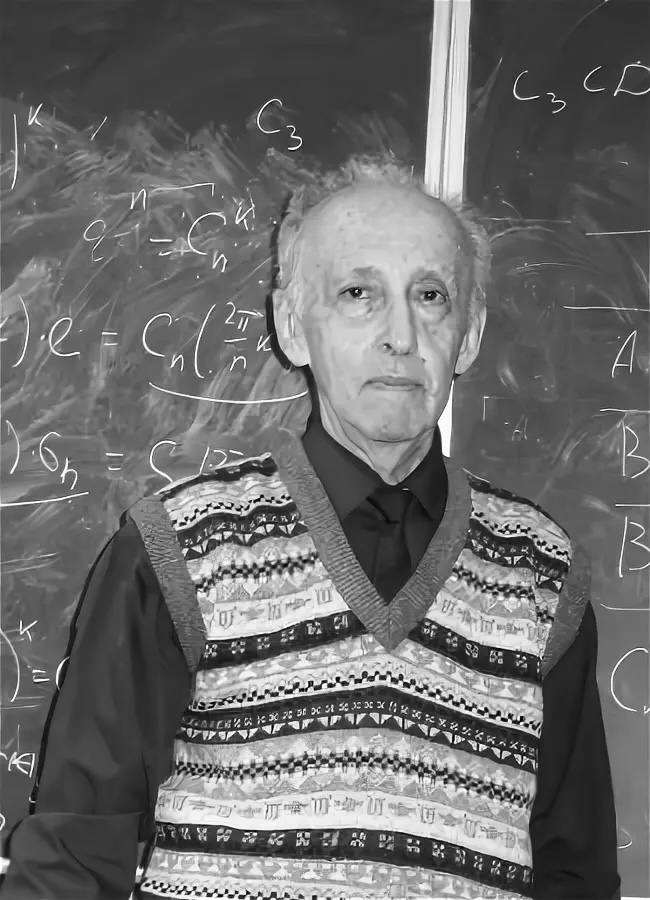
\includegraphics[width=0.264\textwidth]{Zhislin.jpg}}\parbox{0.67\textwidth}{\small\MakeUppercase{\athFA~\athNA}\\ \scriptsize Российский учёный-математик, профессор, д.\,ф.-м.\,н., почетный работник науки и техники РФ. Им получены выдающиеся результаты в области математических задач квантовой механики (исследование спектральных свойств многочастичных гамильтонианов). Теорема о локализации существенного спектра многочастичных систем известна, как теорема Хунцикера--Ван Винтера--Жислина, а теорема о бесконечности дискретного спектра гамильтонианов атомов называется в литературе теоремой Жислина. Автор около 150 научных статей. Член Американского математического общества и Международной ассоциации математической физики. Г.\,М.~Жислин читает общие курсы по математической физике, линейной алгебре и теории групп на факультете <<Высшая школа общей и прикладной физики>> ННГУ.}
		
}}

\newcommand{\lastpage}{
	\clearpage
	\thispagestyle{empty}
	~
	\vfill
	\begin{center}
		\athNA~\textbf{\athFA}
		\ifnum\numAuths>1\\\athNB~\textbf{\athFB}\fi
		\ifnum\numAuths>2\\\athNC~\textbf{\athFC}\fi
		\ifnum\numAuths>3\\\textit{и др.}\fi
		\\[12pt]
		\textbf{\MakeUppercase{\setTitle}.}\\[12pt]
		\setKind \\[24pt]
		Компьютерная верстка -- А.\,Г.~Чубаров\\[12pt]
		Федеральное государственное автономное образовательное учреждение высшего образования\\
		Нижегородский государственный университет им.~Н.И.~Лобачевского.\\
		603950, Нижний Новгород, пр. Гагарина, 23.\\[12pt]		
		Подписано в печать \ \ \ . Формат $60\times84$ 1/16.\\
		Бумага офсетная. Печать офсетная. Гарнитура Computer Modern.\\
		Усл. печ. л. \ \ \ . Уч.-изд. л.\\
		Заказ № \ \ \ \ . Тираж \ \ \ \ экз.\\[12pt]
		Отпечатано в типографии Нижегородского госуниверситета
		им.~Н.И.~Лобачевского.\\
		603600, г. Нижний Новгород, ул. Большая Покровская, 37.
	\end{center}
}

\newcommand{\setTitle}{Лекции по уравнениям математической физики. Часть 1}
% Авторы работы
\newcommand{\numAuths}{1}
% первый автор
\setAuthor{A}{Жислин}{Г.\,М.}{Григорий~Моисеевич}
\newcommand{\allAuths}{Жислин~Г.\,М.}
\newcommand{\setKind}{Учебно-методическое пособие}
% Направление подготовки
\newcommand{\setNapr}{03.04.02 --- Физика}
% Аннотация работы
\newcommand{\setAbstract}{
	Лекции посвящены применению метода разделения переменных (метода Фурье) решения смешанных задач для уравнений в частных производных, которые возникают при описании свободных и вынужденных колебаний струны и мембраны, при описании поведения силы тока и напряжения в проводнике, при нахождении температурных режимов стержней и пластин как при отсутствии источников, так и при их наличии для произвольных начальных и граничных условий. Дан вывод рассматриваемых уравнений.
}
\begin{document}
	\setlength{\abovedisplayskip}{5pt}
	%\setlength{\belowdisplayskip}{5pt}
	\firstpage{\setNapr}
	% вторая страница, аргументы -- УДК, ББК, авторский классификатор, рецензент(ы) направление подготовки
	\secondpage{517.958}{22.311}{Ж-73}{Рецензенты: }
	
	\author{Г.\,М.~Жислин}
	\title{Лекции по уравнениям математической физики. Часть 1}
	\date{Конспектировал А.\,Г.~Чубаров}
	
	
	

	\tableofcontents

	\renewcommand{\thepart}{\Asbuk{part}}
	\renewcommand{\thechapter}{\arabic{chapter}}
	\renewcommand{\thesection}{\arabic{section}.}
	\renewcommand{\thesubsection}{\Roman{subsection}}
	\renewcommand{\thefootnote}{\roman{footnote}}
	\renewcommand{\phi}{\varphi}
	\renewcommand{\Re}{\ensuremath{\mc{R}e\,}}
	\renewcommand{\Im}{\ensuremath{\mc{I}m\,}}
	\renewcommand{\proofname}{Доказательство.}
	\numberwithin{equation}{section}
	\renewcommand{\theequation}{\thesection\arabic{equation}}
	
	\setlength{\intextsep}{0pt}
	\setlength{\textfloatsep}{0pt}
	\chapter*{Введение}
	\phantomsection
	\addcontentsline{toc}{chapter}{Введение}
	\markboth{Введение}{Введение}
	Данный курс --- это первая часть курса <<Методы математической физики>>. Она посвящена в основном описанию и применению метода разделения переменных (метода Фурье) к решению смешанных задач для линейных уравнений в частных производных при произвольных начальных и граничных условиях. Рассматривается решение уравнений, описывающих свободные и вынужденные колебания распределённых систем: струны, мембраны; температурный режим стержней и пластин как при отсутствии источников тепла, так и при их наличии; поведение силы тока и напряжения в проводнике.
	
	Для всех рассмотренных уравнений дан их строгий вывод и доказана единственность решения. Для уравнений, описывающих колебания струны и распространение тепла в стержне определены функции Грина, выяснен их физический смысл, способы построения и применение для решения соответствующих уравнений.
	
	При выводе с помощью принципа Гамильтона уравнения колебаний струны при наличии в точке $\overline{x}$ приложенной сосредоточенной силы или~(и) нагруженной массы методика автора позволила получить для решения уравнения условия в точке $\overline{x}$ как естественные граничные условия.
	
	При решении задачи о колебаниях круглой мембраны мы вновь встречаемся с функциями Бесселя, свойства которых изучались в~\cite{VI}. Здесь мы определяем Гамма-функцию и с её помощью ряды для функций Бесселя отрицательного и дробного порядков. Кроме того мы приводим несколько полезных формул для функций Бесселя. Определяются также модифицированные функции Бесселя, через которые выражаются решения некоторых уравнений при использовании интегральных преобразований.  
	
	Наконец в конце данного пособия мы вводим $\delta$-функцию через $\delta$-по\-следовательности и показываем, как с ними можно работать и как их использовать для построения функций Грина.
	
	Следующие лекции этой части курса посвящены интегральным преобразованиям, но они не вошли в данное пособие так как были изданы раньше~\cite{IP}.
	
	Настоящее пособие представляет собой чуть расширенный конспект лекций, читавшихся автором на факультете ВШ ОПФ нижегородского государственного университета имени Н.\,И.~Лобачевского. Такая форма учебного пособия имеет свои недостатки и, надеюсь, некоторые преимущества. Недостатки (видные автору) заключаются в том, что из-за ограниченности времени и из-за того, что лекции читались не на математическом факультете, многие утверждения не доказываются и ряд математических тонкостей в рассуждениях опускается. С другой стороны подобный подход позволяет выделить главные --- принципиальные~--- моменты в рассказываемом материале и донести до читателя живое слово лектора. Кроме того, тот факт, что конспект лекций сделал слушатель-студент (А.\,Г.~Чубаров), придаёт материалу форму, наиболее удобную для восприятия.
	
	В заключение автор хочет выразить искренно признательность А.\,Г.~Чубарову. Он не только законспектировал лекции, упростил некоторые формулировки, исправил описки, но и набрал весь текст лекций для публикации. Без его помощи данные лекции почти наверняка не были бы изданы.

	\chapter{}
\label{lecture11}

Мы начинаем основную часть курса --- раздел <<уравнения математической физики>>. В этой части мы изучим, во-первых, уравнения, описывающие колебания распределённых систем, во-вторых, уравнения, описывающие распространение тепла в распределённых системах, а также основные методы решения этих --- и не только этих --- уравнений.

\section{Уравнение малых колебаний струны.}
\label{lecture11section1}

\begin{_def}
	Струна --- это гибкая тонкая нить, не сопротивляющаяся изгибу. Внутренние силы возникают в ней только за счёт растяжения.
\end{_def}
Пусть струна в положении равновесия занимает отрезок $[a,b]$ оси $x$, а отклонение точки $x$ в момент $t$ есть $\bm{u}(x,t)$. Для простоты будем считать, что отклонения всех точек $x$ перпендикулярны к отрезку $[a,b]$ и лежат в одной плоскости --- плоскости чертежа и поэтому далее $\bm{u}(x,t)\rightarrow u(x,t)$.

\tikzset{every picture/.style={line width=0.75pt}} %set default line width to 0.75pt        

\begin{tikzpicture}[x=0.75pt,y=0.75pt,yscale=-1,xscale=1]
	%uncomment if require: \path (0,162); %set diagram left start at 0, and has height of 162
	
	%Shape: Axis 2D [id:dp3248327615291966] 
	\draw  (37,131.1) -- (247,131.1)(58,24) -- (58,143) (240,126.1) -- (247,131.1) -- (240,136.1) (53,31) -- (58,24) -- (63,31)  ;
	%Straight Lines [id:da25556170305382886] 
	\draw    (96,136) -- (96,128) ;
	%Straight Lines [id:da25576160043853746] 
	\draw    (207,136) -- (207,128) ;
	%Curve Lines [id:da4799623928387329] 
	\draw    (96,132) .. controls (130,93) and (174,92) .. (207,132) ;
	%Straight Lines [id:da6286410245396021] 
	\draw    (152,86) -- (152,100) ;
	\draw [shift={(152,102)}, rotate = 270] [color={rgb, 255:red, 0; green, 0; blue, 0 }  ][line width=0.75]    (7.65,-2.3) .. controls (4.86,-0.97) and (2.31,-0.21) .. (0,0) .. controls (2.31,0.21) and (4.86,0.98) .. (7.65,2.3)   ;
	%Straight Lines [id:da026907285186595242] 
	\draw    (144,136) -- (144,128) ;
	%Straight Lines [id:da12754670649056732] 
	\draw    (156,136) -- (156,128) ;
	
	% Text Node
	\draw (98,139.4) node [anchor=north west][inner sep=0.75pt]    {$a$};
	% Text Node
	\draw (209,135.4) node [anchor=north west][inner sep=0.75pt]    {$b$};
	% Text Node
	\draw (153,75.4) node [anchor=north west][inner sep=0.75pt]    {$\mathcal{F}$};
	% Text Node
	\draw (142,139.4) node [anchor=north west][inner sep=0.75pt]  [font=\scriptsize]  {$\Delta x$};
	% Text Node
	\draw (247,135.4) node [anchor=north west][inner sep=0.75pt]    {$x$};
	% Text Node
	\draw (8,7.4) node [anchor=north west][inner sep=0.75pt]    {$u( x,t)$};
	
	
\end{tikzpicture}

Чтобы описать колебания струны, то есть движение её точек под действием внутренних и внешних потенциальных сил воспользуемся принципом Гамильтона. Составим интеграл энергии
\begin{equation*}
	\hfill\J[u]=\int\limits_{t_0}^{t_1}\big[T(t)-V(t)\big]\,dt,\hfill
\end{equation*}
где $T$ и $V$ --- кинетическая и потенциальная энергии струны. Найдём первую вариацию $\delta\J$ и затем из равенства $\delta\J=0$ получим уравнение колебаний струны и --- в соответствующих случаях --- граничные условия как ЕГУ (естественные граничные условия).

Пусть струна оттянута от положения равновесия и отпущена. Мы рассматриваем только малые колебания: $|u_x(x,t)|\ll1$.
\begin{gather*}
	\text{Энергия струны }\\
	\qquad\qquad\text{кинетическая}\rightarrow T=T_{\text{р}}+T_{\text{с}},\ V=V_{\text{р}}+V_{\text{с}}\leftarrow\text{потенциальная},
\end{gather*}
\vspace*{-0.8cm}

\noindent где <<р>> и <<с>> означают соответственно энергию распределённой системы и энергию, связанную с сосредоточенным источником. Найдём выражения для $T_{\text{р}},\ T_{\text{с}},\ V_{\text{р}},\ V_{\text{с}}$ начиная с $T_{\text{р}}$. Кинетическая энергия $\Delta T$ элементарного участка $\Delta x$ есть
\begin{equation*}
	\Delta T_{\text{р}}=\Delta m\cdot\frac{u^2_t(x,t)}{2}=\rho\cdot\Delta x\cdot \frac{u^2_t(x,t)}{2},\text{ где $\Delta m$ --- масса участка $\Delta x$, $\rho$ --- плотность струны.}
\end{equation*}  	   
Очевидно, что 
\begin{equation*}
	\hfill T_{\text{р}}=\int\limits_a^{b}\frac{\rho\cdot u^2_t}{2}\,dx.\hfill
\end{equation*}

Энергия $T_{\text{с}}$ присутствует, если струна была нагружена одной или несколькими точечными массами. Предположим, что в точке $\overline{x}$ струна нагружена массой $\overline{m}$. Тогда 
\begin{equation*}
	\hfill T_{\text{с}}=\frac{\overline{m}\cdot u^2_t(\overline{x},t)}{2}.\hfill
\end{equation*}

Переходим к нахождению потенциальной энергии. В общем случае $V_{\text{р}}=V_{\text{р}_1}+V_{\text{р}_2}$, где $V_{\text{р}_1}$ --- потенциальная энергия струны за счёт её растяжения, а $V_{\text{р}_2}$ --- за счёт работы внешних распределённых сил. Начнём сначала с $V_{\text{р}_1}$. Можно доказать (см. например, А.~Тихонов,\,А.~Самарский <<Уравнения математической физики>>), что при малых колебаниях натяжение струны $\mu$ не зависит от удлинения. Поэтому запасённая потенциальная энергия $\Delta V_{\text{р}_1}$ элементарного участка $\Delta x$ пропорциональна его удлинению
\begin{equation*}
	\Delta V_{\text{р}_1}=\mu\cdot\Delta l=\mu\cdot\left(\sqrt{1+u^2_x}\cdot\Delta x-\Delta x\right)\approx\frac{\mu\cdot u^2_x}{2}\cdot\Delta x.\footnotemark{} 
\end{equation*}
\footnotetext{здесь мы воспользовались приближённой формулой $\sqrt{1+\alpha}\approx 1+\frac{\alpha}{2}$, при $|\alpha|\ll1$.}Следовательно
\begin{equation*}
	\hfill V_{\text{р}_1}=\int\limits_a^b\frac{\mu\cdot u^2_x}{2}\,dx.\hfill
\end{equation*}

Найдём $V_{\text{р}_2}$. Пусть на струну действует распределённая сила $\mc{F}$ направленная перпендикулярно к $[a,b]$ в плоскости чертежа и пусть $f(x,t)$ --- линейная плотность этой силы, то есть $f(x,t)$ есть сила, действующая на единицу длины. Сила, действующая на элементарный участок $\Delta x$ --- $\Delta\mc{F}=f\cdot\Delta x$ и поэтому её потенциал $\Delta U=-f(x,t)\cdot\Delta x\cdot u(x,t)$. Следовательно, потенциальная энергия участка $\Delta x$ за счёт силы $\mc{F}$ есть $\Delta V_{\text{р}_2}=\Delta U=-f\cdot u\cdot\Delta x$, а полная потенциальная энергия за счёт действия силы $\mc{F}$ очевидно
\begin{equation*}
	\hfill V_{\text{р}_2}=-\int\limits_a^b f\cdot u\,dx.\footnotemark{}\hfill
\end{equation*}
\footnotetext{Здесь мы воспользовались известным из курсов физики фактом, что когда внешняя сила действует на объект, то изменение потенциальной энергии объекта равно потенциалу силы.}

Обсудим теперь величину $V_{\text{с}}$. Предположим, что в точке $\widehat{x}$ на струну действует сосредоточенная сила, перпендикулярная отрезку $[a,b]$ или же (или одновременно) в этой точке к струне прикреплена пружина, которую струна сжимает или растягивает при колебаниях.

\tikzset{every picture/.style={line width=0.75pt}} %set default line width to 0.75pt        

\begin{tikzpicture}[x=0.75pt,y=0.75pt,yscale=-1,xscale=1]
	%uncomment if require: \path (0,162); %set diagram left start at 0, and has height of 162
	
	%Shape: Axis 2D [id:dp568415431333978] 
	\draw  (37,131.1) -- (247,131.1)(58,24) -- (58,143) (240,126.1) -- (247,131.1) -- (240,136.1) (53,31) -- (58,24) -- (63,31)  ;
	%Straight Lines [id:da6315311561256083] 
	\draw    (96,136) -- (96,128) ;
	%Straight Lines [id:da07005979202360346] 
	\draw    (207,136) -- (207,128) ;
	%Curve Lines [id:da644520411610563] 
	\draw    (96,132) .. controls (128,89.5) and (171,80.5) .. (207,132) ;
	%Straight Lines [id:da660057766915144] 
	\draw    (159,136) -- (159,128) ;
	%Shape: Spring [id:dp1849279727639963] 
	\draw   (157.29,97.43) .. controls (159.32,97.69) and (161.35,98.7) .. (161.33,100.7) .. controls (161.31,104.7) and (153.18,104.65) .. (153.19,102.65) .. controls (153.21,100.65) and (161.33,100.7) .. (161.31,104.7) .. controls (161.28,108.7) and (153.15,108.65) .. (153.17,106.65) .. controls (153.18,104.65) and (161.31,104.7) .. (161.28,108.7) .. controls (161.25,112.7) and (153.12,112.65) .. (153.14,110.65) .. controls (153.15,108.65) and (161.28,108.7) .. (161.25,112.7) .. controls (161.22,116.7) and (153.1,116.65) .. (153.11,114.65) .. controls (153.12,112.65) and (161.25,112.7) .. (161.22,116.7) .. controls (161.19,120.7) and (153.07,120.65) .. (153.08,118.65) .. controls (153.1,116.65) and (161.22,116.7) .. (161.19,120.7) .. controls (161.17,124.7) and (153.04,124.65) .. (153.05,122.65) .. controls (153.07,120.65) and (161.19,120.7) .. (161.17,124.7) .. controls (161.14,128.7) and (153.01,128.65) .. (153.03,126.65) .. controls (153.04,124.65) and (161.17,124.7) .. (161.14,128.7) .. controls (161.11,132.7) and (152.99,132.65) .. (153,130.65) .. controls (153.01,128.65) and (161.14,128.7) .. (161.11,132.7) .. controls (161.08,136.7) and (152.96,136.65) .. (152.97,134.65) .. controls (152.99,132.65) and (161.11,132.7) .. (161.08,136.7) .. controls (161.05,140.7) and (152.93,140.65) .. (152.94,138.65) .. controls (152.96,136.65) and (161.08,136.7) .. (161.05,140.7) .. controls (161.03,144.7) and (152.9,144.65) .. (152.92,142.65) .. controls (152.93,140.65) and (161.05,140.7) .. (161.03,144.7) .. controls (161,148.7) and (152.87,148.65) .. (152.89,146.65) .. controls (152.9,144.68) and (160.75,144.7) .. (160.99,148.5) ;
	%Straight Lines [id:da04984138320568832] 
	\draw [line width=2.25]    (147,150.5) -- (166,150.5) ;
	
	% Text Node
	\draw (98,135.4) node [anchor=north west][inner sep=0.75pt]    {$a$};
	% Text Node
	\draw (209,135.4) node [anchor=north west][inner sep=0.75pt]    {$b$};
	% Text Node
	\draw (247,135.4) node [anchor=north west][inner sep=0.75pt]    {$x$};
	% Text Node
	\draw (170,135.4) node [anchor=north west][inner sep=0.75pt]    {$\hat{x}$};
	
	
\end{tikzpicture}

Обозначим изменение энергии струны в точке $\widehat{x}$ через $g$. Выражение для $g$ будет дано позже, а пока только для упрощения дальнейших выкладок предположим, что $\widehat{x}=\overline{x}$. Таким образом
\begin{equation*}
	\hfill V_{\text{с}}=g(t,u(\overline{x},t)).\hfill
\end{equation*}

Собирая вместе все составляющие кинетической и потенциальной энергии струны, мы получим интеграл действия в виде
\begin{equation*}
	\hfill \J[u]=\int\limits_{t_0}^{t_1}\!\!\int\limits_a^b\underbrace{\left(\frac{\rho\cdot u^2_t}{2}-\frac{\mu\cdot u^2_x}{2}+f\cdot u\right)}_{F}\,dxdt+\int\limits_{t_0}^{t_1}\underbrace{\left(\frac{\overline{m}\cdot u^2_t(\overline{x},t)}{2}-g(t,u(\overline{x},t))\right)}_{\Phi}\,dt\hfill
\end{equation*}
Обозначим подынтегральное выражение двукратного интеграла через $F=F(x,t,u,u_x,u_t)$, а однократного через $\Phi=\Phi(t,u(\overline{x},t),u_t(\overline{x},t))$ и введём на плоскости $x,t$ область 
\begin{equation*}
	\Omega=\left\{x,t|\, x\in[a,b],\, t\in[t_0,t_1]\right\}
\end{equation*}

\tikzset{every picture/.style={line width=0.75pt}} %set default line width to 0.75pt        

\begin{tikzpicture}[x=0.75pt,y=0.75pt,yscale=-1,xscale=1]
	%uncomment if require: \path (0,162); %set diagram left start at 0, and has height of 162
	
	%Shape: Axis 2D [id:dp033385002892103444] 
	\draw  (37,131.1) -- (247,131.1)(58,24) -- (58,143) (240,126.1) -- (247,131.1) -- (240,136.1) (53,31) -- (58,24) -- (63,31)  ;
	%Straight Lines [id:da23290127141076722] 
	\draw    (96,136) -- (96,128) ;
	%Straight Lines [id:da9776319010753525] 
	\draw    (207,136) -- (207,128) ;
	%Straight Lines [id:da06420289301641557] 
	\draw    (151,136) -- (151,128) ;
	%Shape: Rectangle [id:dp34760015951663625] 
	\draw   (96,58) -- (207,58) -- (207,109) -- (96,109) -- cycle ;
	%Straight Lines [id:da011040244644266117] 
	\draw    (53,109) -- (62,109) ;
	%Straight Lines [id:da4964088587876916] 
	\draw    (53,58) -- (62,58) ;
	%Straight Lines [id:da2828961469522162] 
	\draw    (113,28.5) -- (131.74,51.45) ;
	\draw [shift={(133,53)}, rotate = 230.77] [color={rgb, 255:red, 0; green, 0; blue, 0 }  ][line width=0.75]    (10.93,-3.29) .. controls (6.95,-1.4) and (3.31,-0.3) .. (0,0) .. controls (3.31,0.3) and (6.95,1.4) .. (10.93,3.29)   ;
	%Straight Lines [id:da2101032473064448] 
	\draw    (151,57.5) -- (151,109) ;
	
	% Text Node
	\draw (98,137.4) node [anchor=north west][inner sep=0.75pt]    {$a$};
	% Text Node
	\draw (209,135.4) node [anchor=north west][inner sep=0.75pt]    {$b$};
	% Text Node
	\draw (247,135.4) node [anchor=north west][inner sep=0.75pt]    {$x$};
	% Text Node
	\draw (41,14.4) node [anchor=north west][inner sep=0.75pt]    {$t$};
	% Text Node
	\draw (153,135.4) node [anchor=north west][inner sep=0.75pt]    {$\overline{x}$};
	% Text Node
	\draw (35,101.4) node [anchor=north west][inner sep=0.75pt]    {$t_{0}$};
	% Text Node
	\draw (35,53.4) node [anchor=north west][inner sep=0.75pt]    {$t_{1}$};
	% Text Node
	\draw (81,101.4) node [anchor=north west][inner sep=0.75pt]    {$A$};
	% Text Node
	\draw (81,49.4) node [anchor=north west][inner sep=0.75pt]    {$D$};
	% Text Node
	\draw (208,101.4) node [anchor=north west][inner sep=0.75pt]    {$B$};
	% Text Node
	\draw (208,49.4) node [anchor=north west][inner sep=0.75pt]    {$C$};
	% Text Node
	\draw (97,14.4) node [anchor=north west][inner sep=0.75pt]    {$\Omega $};
	% Text Node
	\draw (144,111.4) node [anchor=north west][inner sep=0.75pt]  [font=\scriptsize]  {$M$};
	% Text Node
	\draw (144,45.4) node [anchor=north west][inner sep=0.75pt]  [font=\scriptsize]  {$N$};
	% Text Node
	\draw (115,75.4) node [anchor=north west][inner sep=0.75pt]    {$\Omega _{1}$};
	% Text Node
	\draw (170,75.4) node [anchor=north west][inner sep=0.75pt]    {$\Omega _{2}$};
	
	
\end{tikzpicture}
\begin{equation*}
	\text{Тогда }\J[u]=\iint\limits_{\Omega}F\,dxdt+\int\limits_{M}^{N}\Phi\,dt\text{, где }M=(\overline{x},t_0),\ N=(\overline{x},t_1).
\end{equation*}

\noindent Чтобы найти вариацию от интеграла действия, то есть величину $\displaystyle\gamma\cdot\left.\der{}{\gamma}\J[u+\gamma\cdot\eta]\right|_{\gamma=0}$ надо в первую очередь ввести допустимое изменение $\eta(x,t)$ и описать его свойства исходя из того, что функция $u(x,t)+\gamma\cdot\eta(x,t)$ ($\gamma$ --- малый параметр) должна описывать траекторию движения струны из того же начального состояния в то же конечное, что и $u(x,t)$. Так как состояние струны определяется положением каждой точки, то мы потребуем, чтобы  
\begin{equation*}
	\hfill \eta(x,t_0)=\eta(x,t_1)\equiv0,\quad\forall x\in[a,b].\hfill
\end{equation*}

Далее при нахождении первой вариации двукратных интегралов в лекции по <<вариационному исчислению>> мы применяли формулу Остроградского--Гаусса к вектору вида $\bm{W}=\big(F_{u_x}\cdot\eta,F_{u_t}\cdot\eta\big)$\footnote{Там производная была не по $t$, а по $y$, но это не существенно.}. Но применение данной формулы возможно лишь при определённой гладкости компонент этого вектора, а в рассматриваемой ситуации функция $u_x(x,t)$, а следовательно и компоненты вектора $\bm{W}$ могут иметь разрыв при $x=\overline{x}$. Поэтому при нахождении первой вариации интеграла действия мы разобьём область $\Omega$ на две области
\begin{equation*}
	\Omega_{1}=\left\{x,t|\,x\in[a,\overline{x}],\ t\in[t_0,t_1]\right\},\quad	\Omega_{2}=\left\{x,t|\,x\in(\overline{x},b],\ t\in[t_0,t_1]\right\}
\end{equation*} 
и будем брать вариацию по каждой из областей. Имеем 
\begin{equation*}
	\J[u]=\iint\limits_{\Omega_1}F\,dxdt+\iint\limits_{\Omega_2}F\,dxdt+\int\limits_{M}^{N}\Phi\,dt.
\end{equation*}
Предположим, что $a<\overline{x}<b$ и что концы струны или закреплены $u(a,t)=u(b,t)=0$, или движутся по заданным законам $u(a,t)=\nu_1(t)$, $u(b,t)=\nu_2(t)$. В обоих случаях мы должны потребовать, чтобы 
\begin{equation*}
	\hfill\eta(a,t)=\eta(b,t)\equiv0,\quad\forall t.\hfill
\end{equation*}
Если же $\overline{x}=a\,\{b\}$, то области $\Omega_{1}\,\{\Omega_{2}\}$ не будет, и тогда требование $\eta(a,t)\equiv0\,\{\eta(b,t)\equiv0\}$ отпадает
\begin{equation*}
	\text{Положим  }\J_j[u]=\iint\limits_{\Omega_j}F(x,t,u,u_x,u_t)\,dxdt,\ j=1,2;\quad\J_3[u]=\int\limits_{t_0}^{t_1}\Phi(t,u(\overline{x},t),u_t(\overline{x},t))\,dt 
\end{equation*}
\begin{gather*}
	\text{Тогда  }\J[u]=\J_1[u]+\J_2[u]+\J_3[u]
	\intertext{и}
	\delta\J=\gamma\cdot\left.\der{}{\gamma}\left\{\sum\limits_{j=1}^2\J_{j}[u+\gamma\cdot\eta]+\J_3[u+\gamma\cdot\eta(\overline{x},t)]\right\}\right|_{\gamma=0\ \displaystyle.}
\end{gather*}
Используя известные нам формулы первой вариации для двукратных и однократных интегралов получим
\begin{multline}
	\label{l11:eq:1}
	\delta\J=\gamma\cdot\left[\vphantom{\iint\limits_{\Omega_j}}\right.\sum\limits_{j=1}^2\left\{\iint\limits_{\Omega_j}\left(F_{u}-\der{}{x}F_{u_x}-\der{}{t}F_{u_t}\right)\cdot\eta\,dxdt+\int\limits_{\partial\Omega_j}\left(F_{u_x}\cdot\cos\alpha+F_{u_t}\cdot\cos\beta\right)\cdot\eta\,dl\right\}+\\
	+\int\limits_{t_0}^{t_1}\left(\Phi_{u}-\der{}{t}\Phi_{u_t}\right)\cdot\eta(\overline{x},t)\,dt+\Phi_{u_t}\cdot\eta(\overline{x},t)\mathop{\Big|}\limits_{t_0}^{t_1}\left.\vphantom{\iint\limits_{\Omega_j}}\right]_{\displaystyle.}
\end{multline}
Здесь $\cos\alpha$, $\cos\beta$ --- компоненты единичной внешней нормали к границе области $\Omega_j$ на плоскости $x,t$.

\tikzset{every picture/.style={line width=0.75pt}} %set default line width to 0.75pt        

\begin{tikzpicture}[x=0.75pt,y=0.75pt,yscale=-1,xscale=1]
	%uncomment if require: \path (0,162); %set diagram left start at 0, and has height of 162
	
	%Shape: Axis 2D [id:dp2237198969795473] 
	\draw  (37,131.1) -- (247,131.1)(58,24) -- (58,143) (240,126.1) -- (247,131.1) -- (240,136.1) (53,31) -- (58,24) -- (63,31)  ;
	%Straight Lines [id:da4988233348557616] 
	\draw    (96,136) -- (96,128) ;
	%Straight Lines [id:da3469178817338765] 
	\draw    (207,136) -- (207,128) ;
	%Straight Lines [id:da48617665238907604] 
	\draw    (151,136) -- (151,128) ;
	%Shape: Rectangle [id:dp8926884831137676] 
	\draw   (96,58) -- (207,58) -- (207,109) -- (96,109) -- cycle ;
	%Straight Lines [id:da23169370164602432] 
	\draw    (53,109) -- (62,109) ;
	%Straight Lines [id:da7909330230568588] 
	\draw    (53,58) -- (62,58) ;
	%Straight Lines [id:da17521553787578226] 
	\draw    (151,57.5) -- (151,109) ;
	
	% Text Node
	\draw (98,137.4) node [anchor=north west][inner sep=0.75pt]    {$a$};
	% Text Node
	\draw (209,135.4) node [anchor=north west][inner sep=0.75pt]    {$b$};
	% Text Node
	\draw (247,135.4) node [anchor=north west][inner sep=0.75pt]    {$x$};
	% Text Node
	\draw (41,14.4) node [anchor=north west][inner sep=0.75pt]    {$t$};
	% Text Node
	\draw (153,135.4) node [anchor=north west][inner sep=0.75pt]    {$\overline{x}$};
	% Text Node
	\draw (35,101.4) node [anchor=north west][inner sep=0.75pt]    {$t_{0}$};
	% Text Node
	\draw (35,53.4) node [anchor=north west][inner sep=0.75pt]    {$t_{1}$};
	% Text Node
	\draw (81,101.4) node [anchor=north west][inner sep=0.75pt]    {$A$};
	% Text Node
	\draw (81,49.4) node [anchor=north west][inner sep=0.75pt]    {$D$};
	% Text Node
	\draw (208,101.4) node [anchor=north west][inner sep=0.75pt]    {$B$};
	% Text Node
	\draw (208,49.4) node [anchor=north west][inner sep=0.75pt]    {$C$};
	% Text Node
	\draw (144,111.4) node [anchor=north west][inner sep=0.75pt]  [font=\scriptsize]  {$M$};
	% Text Node
	\draw (144,45.4) node [anchor=north west][inner sep=0.75pt]  [font=\scriptsize]  {$N$};
	% Text Node
	\draw (115,75.4) node [anchor=north west][inner sep=0.75pt]    {$\Omega _{1}$};
	% Text Node
	\draw (170,75.4) node [anchor=north west][inner sep=0.75pt]    {$\Omega _{2}$};
	
	
\end{tikzpicture}

Так как $\eta(x,t_0)=\eta(x,t_1)=0\,\forall x$, то интегралы по границам областей $\Omega_j$ сведутся к интегралам по $M\!N$ и $D\!A$ для $\Omega_1$ и по $BC$ и $N\!M$ для $\Omega_2$\footnote{Напомним, что положительное направление обхода границы --- обход против часовой стрелки.}. Очевидно, что на отрезках $BC$, $M\!N$, $N\!M$, $D\!A$ выполняется $\cos\beta=0$, так как нормали к ним перпендикулярны к оси $t$. Далее $\cos\alpha=1$ на $BC$ и $M\!N$ и $\cos\alpha=-1$ на $D\!A$ и $N\!M$.

Учитывая вышесказанное и полагая для краткости $P\eqdef\big(F_{u_x}\cdot\cos\alpha+F_{u_t}\cdot\cos\beta\big)\cdot\eta$, имеем
\begin{multline}
	\label{l11:eq:2}
	\int\limits_{\partial\Omega_1}P\,dl=\int\limits_{t_0}^{t_1}P\bigg|_{\lefteqn{\scriptstyle x=\overline{x}-0}}\,dt\quad+\int\limits_{t_1}^{t_0}P\bigg|_{\lefteqn{\scriptstyle x=a+0}}\,dl\quad=\int\limits_{t_0}^{t_1}P\bigg|_{\lefteqn{\scriptstyle x=\overline{x}-0}}\,dt\quad+\int\limits_{t_0}^{t_1}P\bigg|_{\lefteqn{\scriptstyle x=a+0}}\,dt\quad=\\
	=\int\limits_{t_0}^{t_1}\left[\mu\cdot u_x\bigg|_{\lefteqn{\scriptstyle x=a+0}}\cdot\eta(a,t)-\mu\cdot u_x\bigg|_{\lefteqn{\scriptstyle x=\overline{x}-0}}\cdot\eta(\overline{x},t)\right]\,dt.
\end{multline}  
\begin{equation}
	\label{l11:eq:3}
	\int\limits_{\partial\Omega_2}P\,dl=\int\limits_{t_0}^{t_1}P\bigg|_{\lefteqn{\scriptstyle x=b-0}}\,dt\quad+\int\limits_{t_1}^{t_0}P\bigg|_{\lefteqn{\scriptstyle x=\overline{x}+0}}\,dl\quad=\int\limits_{t_0}^{t_1}\left[-\mu\cdot u_x\bigg|_{\lefteqn{\scriptstyle x=b-0}}\cdot\eta(b,t)+\mu\cdot u_x\bigg|_{\lefteqn{\scriptstyle x=\overline{x}+0}}\cdot\eta(\overline{x},t)\right]\,dt.
\end{equation}
Здесь учтено, что $dl=dt$ при интегрировании по $BC$, $M\!N$ и $dl=-dt$ при интегрировании по $N\!M$ и $D\!A$.

Перепишем теперь выражение \eqref{l11:eq:1}, подставляя туда $F$ и $\Phi$. Тогда с учётом равенств \eqref{l11:eq:2} и \eqref{l11:eq:3} получим
\begin{multline}
	\label{l11:eq:4}
	\delta\J=\gamma\cdot\left\{\vphantom{\iint\limits_{\Omega_j}}\right.\!\sum\limits_{j=1}^{2}\iint\limits_{\Omega_j}\left[f+\pder{}{x}\big(\mu\cdot u_x\big)-\pder{}{t}\big(\rho\cdot u_t\big)\right]\cdot\eta\,dxdt+\\
	+\int\limits_{t_0}^{t_1}\left[\mu\cdot u_x\cdot\eta\bigg|_{x=a+0}-\mu\cdot u_x\cdot\eta\bigg|_{x=\overline{x}-0}-\mu\cdot u_x\cdot\eta\bigg|_{x=b-0}+\mu\cdot u_x\cdot\eta\bigg|_{x=\overline{x}+0}-\big(\overline{m}\cdot u_{tt}+g_u\big)\cdot\eta\bigg|_{x=\overline{x}}\,\right]\,dt\!\left.\vphantom{\iint\limits_{\Omega_j}}\right\}_{\displaystyle.}
\end{multline}
Взяв $\eta(a,t)=\eta(b,t)=\eta(\overline{x},t)=0$ и затем $\eta(x,t)\equiv0$, при $(x,t)\in\Omega_2$ получим условие $\delta\J=0$ в виде 
\begin{equation*}
	\hfill\iint\limits_{\Omega_1}\left[f+\pder{}{x}\big(\mu\cdot u_x\big)-\pder{}{t}\big(\rho\cdot u_t\big)\right]\cdot\eta\,dxdt=0.\hfill
\end{equation*}
Отсюда по лемме Лагранжа для функций двух переменных получаем 
\begin{equation}
	\label{l11:eq:5}
	\hfill f+\pder{}{x}\big(\mu\cdot u_x\big)-\pder{}{t}\big(\rho\cdot u_t\big)=0\quad\text{при }(x,t)\in\Omega_1.\hfill
\end{equation}
Аналогично полагая $\eta(x,t)\equiv0$ в области $\Omega_1$, убеждаемся в справедливости уравнения~\eqref{l11:eq:5} для $(x,t)\in\Omega_2$, исключая, быть может, отрезок $x=\overline{x}$, $t\in[t_0,t_1]$. Уравнение~\eqref{l11:eq:5} --- это и есть уравнение колебаний струны.

Если $\overline{x}\neq a,b$, то взяв $\eta(a,t)=\eta(b,t)=0$ мы в силу~\eqref{l11:eq:4} с учётом~\eqref{l11:eq:5} получим
\begin{equation*}
	\int\limits_{t_0}^{t_1}\left[\mu\cdot u_x\bigg|_{x=\overline{x}+0}-\mu\cdot u_x\bigg|_{x=\overline{x}-0}-\overline{m}\cdot u_{tt}(\overline{x},t)-g_u\bigg|_{x=\overline{x}}\right]\cdot\eta(\overline{x},t)=0\quad\forall \eta(\overline{x},t).
\end{equation*}
Отсюда в силу леммы Лагранжа для однократных интегралов получаем условие при $x=\overline{x}$
\begin{equation}
	\label{l11:eq:6}
	\hfill \mu\cdot u_x\bigg|_{x=\overline{x}+0}-\mu\cdot u_x\bigg|_{x=\overline{x}-0}-\big(\overline{m}\cdot u_{tt}+g_u\big)\bigg|_{x=\overline{x}}=0\hfill
\end{equation}
Вид функции $g$ мы обсудим позже, а пока рассмотрим случаи $\overline{x}=a$ и $\overline{x}=b$. Пусть $\overline{x}=a$, тогда области $\Omega_1$ не будет, и~\eqref{l11:eq:6} запишется в виде 
\begin{equation}
	\label{l11:eq:7}
	\hfill\mu\cdot u_x\bigg|_{x=a}=\big(\overline{m}\cdot u_{tt}+g_u\big)\bigg|_{x=a}\hfill
\end{equation}
при $\overline{x}=b$ нет области $\Omega_2$ и условие~\eqref{l11:eq:6} можно переписать в виде 
\begin{equation}
	\label{l11:eq:8}
	\hfill-\mu\cdot u_x\bigg|_{x=b}=\big(\overline{m}\cdot u_{tt}+g_u\big)\bigg|_{x=b}\hfill
\end{equation} 

Найдём теперь вид функции $g(t,u(\overline{x},t))$ для двух наиболее интересных случаев.
\begin{enumerateA}
	\item\label{l11:enum:A} Пусть в точке $\overline{m}$ действует сосредоточенная сила $f_0(t)$. Потенциал $v_0(t)$ этой силы, очевидно, равен --- $f_0(t)\cdot u(\overline{x},t)$ и, следовательно, $g=v_0=-f_0(t)\cdot u(\overline{x},t)$. В этом случае $g_u=-f_0(t)$ и тогда при $\overline{m}=0$ условие~\eqref{l11:eq:6} перепишется в виде 
	\addtocounter{equation}{-2}
	\begin{equation}
		\label{l11:eq:6A}
		\hfill\mu\cdot u_x\bigg|_{\overline{x}+0}-\mu\cdot u_x\bigg|_{\overline{x}-0}=-f_0(t), \tag{\theequation{}A}\hfill
	\end{equation} 
	а условия \eqref{l11:eq:7} и \eqref{l11:eq:8} в виде
	\addtocounter{equation}{1} 
	\begin{equation}
		\label{l11:eq:7A}
		\hfill\mu\cdot u_x\bigg|_{x=a}=-f_1(t),\tag{\theequation{}A}\hfill
	\end{equation}
	\vspace{-0.2cm}\addtocounter{equation}{1}
	\begin{equation}
		\label{l11:eq:8A}
		\hfill\mu\cdot u_x\bigg|_{x=b}=f_2(t),\tag{\theequation{}A}\hfill
	\end{equation}
	где $f_1(t)$ и $f_2(t)$ --- сосредоточенные силы, действующие на концах струны. 
	
	\noindent Если $f_1(t)=f_2(t)\equiv0$, то мы получим условия на свободных концах
	\begin{equation}
		\label{l11:eq:9}
		\hfill \mu\cdot u_x\bigg|_{x=a}=0,\quad\mu\cdot u_x\bigg|_{x=b}=0.\hfill
	\end{equation}
	Отметим, что условие \eqref{l11:eq:6A} описывает скачок производной $u_x$ в точке $x=\overline{x}$.
	\item Упругое закрепление. Пусто в точке $x=\overline{x}$ к струне прикреплена пружинка, натянутая на вертикальный стержень (без трения) и закреплённая в точке $C$.
	
	\tikzset{every picture/.style={line width=0.75pt}} %set default line width to 0.75pt        
	
	\begin{tikzpicture}[x=0.75pt,y=0.75pt,yscale=-1,xscale=1]
		%uncomment if require: \path (0,162); %set diagram left start at 0, and has height of 162
		
		%Shape: Axis 2D [id:dp3800136695378986] 
		\draw  (37,131.1) -- (247,131.1)(58,24) -- (58,143) (240,126.1) -- (247,131.1) -- (240,136.1) (53,31) -- (58,24) -- (63,31)  ;
		%Straight Lines [id:da6326916483448484] 
		\draw    (96,136) -- (96,128) ;
		%Straight Lines [id:da6653494140567895] 
		\draw    (207,136) -- (207,128) ;
		%Curve Lines [id:da29314973980873904] 
		\draw    (96,132) .. controls (128,89.5) and (171,80.5) .. (207,132) ;
		%Shape: Spring [id:dp9827771082396111] 
		\draw   (156.29,97.43) .. controls (158.32,97.69) and (160.35,98.7) .. (160.33,100.7) .. controls (160.31,104.7) and (152.18,104.65) .. (152.19,102.65) .. controls (152.21,100.65) and (160.33,100.7) .. (160.31,104.7) .. controls (160.28,108.7) and (152.15,108.65) .. (152.17,106.65) .. controls (152.18,104.65) and (160.31,104.7) .. (160.28,108.7) .. controls (160.25,112.7) and (152.12,112.65) .. (152.14,110.65) .. controls (152.15,108.65) and (160.28,108.7) .. (160.25,112.7) .. controls (160.22,116.7) and (152.1,116.65) .. (152.11,114.65) .. controls (152.12,112.65) and (160.25,112.7) .. (160.22,116.7) .. controls (160.19,120.7) and (152.07,120.65) .. (152.08,118.65) .. controls (152.1,116.65) and (160.22,116.7) .. (160.19,120.7) .. controls (160.17,124.7) and (152.04,124.65) .. (152.05,122.65) .. controls (152.07,120.65) and (160.19,120.7) .. (160.17,124.7) .. controls (160.14,128.7) and (152.01,128.65) .. (152.03,126.65) .. controls (152.04,124.65) and (160.17,124.7) .. (160.14,128.7) .. controls (160.11,132.7) and (151.99,132.65) .. (152,130.65) .. controls (152.01,128.65) and (160.14,128.7) .. (160.11,132.7) .. controls (160.08,136.7) and (151.96,136.65) .. (151.97,134.65) .. controls (151.99,132.65) and (160.11,132.7) .. (160.08,136.7) .. controls (160.05,140.7) and (151.93,140.65) .. (151.94,138.65) .. controls (151.96,136.65) and (160.08,136.7) .. (160.05,140.7) .. controls (160.03,144.7) and (151.9,144.65) .. (151.92,142.65) .. controls (151.93,140.65) and (160.05,140.7) .. (160.03,144.7) .. controls (160,148.7) and (151.87,148.65) .. (151.89,146.65) .. controls (151.9,144.68) and (159.75,144.7) .. (159.99,148.5) ;
		%Straight Lines [id:da34764408804486013] 
		\draw [line width=2.25]    (147,150.5) -- (166,150.5) ;
		
		% Text Node
		\draw (98,135.4) node [anchor=north west][inner sep=0.75pt]    {$a$};
		% Text Node
		\draw (209,135.4) node [anchor=north west][inner sep=0.75pt]    {$b$};
		% Text Node
		\draw (247,135.4) node [anchor=north west][inner sep=0.75pt]    {$x$};
		% Text Node
		\draw (167,145.4) node [anchor=north west][inner sep=0.75pt]    {$C$};
		
		
	\end{tikzpicture}
	
	При колебаниях струна работает, растягивая или сжимая пружинку. Сила, необходимая для смещения конца пружинки на величину $u(\overline{x},t)$ по закону Гука есть
	\begin{equation*}
		f_0(\overline{x},t)=k\cdot u(\overline{x},t)\text{, где }k\text{ --- характеризует жёсткость пружины.} 
	\end{equation*}
	\begin{equation*}
		\text{Потенциал этой силы, очевидно, равен }v_0=-\frac{k\cdot u^2(\overline{x},t)}{2}.
	\end{equation*}
	
	В отличие от рассмотренных ранее случаев, когда внешние силы (распределённые или сосредоточенные) действовали на струну, в рассматриваемой ситуации работает сама струна. Поэтому здесь потенциальная энергия струны $g=-v_0$\footnote{Напомним, что в случае \ref{l11:enum:A} выполнялось $g=v_0$.}, то есть $g(t,u(\overline{x},t))=k\cdot u^2(\overline{x},t)\bigm/2$ и $g_u(t,u(\overline{x},t))=k\cdot u(\overline{x},t)$. Поэтому условие~\eqref{l11:eq:6} при $\overline{m}=0$ запишется в виде\addtocounter{equation}{-3}
	\begin{equation}
		\label{l11:eq:6B}
		\hfill\mu\cdot u_x\bigg|_{\overline{x}+0}-\mu\cdot u_x\bigg|_{\overline{x}-0}=k\cdot u. \tag{\theequation{}B}\hfill
	\end{equation}  
	Если упруго закреплены концы струны и $k_1$, $k_2$ --- коэффициенты жёсткости соответствующих пружин, то из~\eqref{l11:eq:7} и~\eqref{l11:eq:8} при $\overline{m}=0$ мы получим условия упругого закрепления концов струны:
	\addtocounter{equation}{1} 
	\begin{equation}
		\label{l11:eq:7B}
		\hfill\mu\cdot u_x\bigg|_{x=a}=k_1\cdot u\bigg|_{x=a},\tag{\theequation{}B}\hfill
	\end{equation}
	\vspace{-0.2cm}\addtocounter{equation}{1}
	\begin{equation}
		\label{l11:eq:8B}
		\hfill\mu\cdot u_x\bigg|_{x=b}=-k_2\cdot u\bigg|_{x=b},\tag{\theequation{}B}\hfill
	\end{equation}
	\addtocounter{equation}{1} 
	
	Граничные условия для разных ситуаций на концах струны надо знать! Заметим в заключение, что наряду с этими условиями возможен случай, когда заданы законы движения концов струны
	\begin{equation*}
		\hfill u(a,t)=h_1(t)\text{ и }u(b,t)=h_2(t),\hfill
	\end{equation*} 
	где $h_i(t)$ --- известные функции.
\end{enumerateA}
		\chapter{}
\label{lecture12}
\section{Уравнение малых колебаний струны (продолжение).}
\label{lecture12section1}
\markboth{Лекция~\thechapter.}{\thesection\quad Уравнение малых колебаний струны.}%
Возвращаемся к выведенному нами уравнению колебаний струны
\begin{equation}
	\label{l12:eq:1}
	\pder{}{x}\big(\mu\cdot u_x\big)-\pder{}{t}\big(\rho\cdot u_t\big)+f(x,t)=0.
\end{equation}
Пусть начальное положение и начальная скорость струны задаются равенствами 
\begin{equation}
	\label{l12:eq:2}
	 u(x,0)=\phi(x),\quad u_t(x,0)=\psi(x),
\end{equation} 
где $\phi(x)$ и $\psi(x)$ --- известные функции. Граничные условия возьмём простейшие --- предположим, что концы струны закреплены.
\begin{equation}
	\label{l12:eq:3}
	 u(a,t)=0,\quad u(b,t)=0.
\end{equation}

При постановке задач, приводящих к уравнениям в частных производных (так же как в задачах, связанных с обыкновенными дифференциальными уравнениями) огромное значение имеет \emph{корректность постановки задачи}.
\begin{Def}
	Мы говорим, что \textbf{задача поставлена корректно}, если для рассматриваемого уравнения решение:
	\begin{enumerateD}
		\item существует;
		\item единственно;
		\item непрерывно зависит от входных данных.
	\end{enumerateD} 
\end{Def}
\noindent Поясним сказанное в основном применительно к задаче~\eqref{l12:eq:1}--\eqref{l12:eq:3}.
\begin{enumerateD}
	\item На практике существование решения большей частью доказывается прямым его построением. Но решение может не существовать, если наложить избыточные требования. Приведём два примера.
	\begin{enumerateD}
		\item Пусть решение уравнения~\eqref{l12:eq:1} ищется в классе $\Cfn{2}(\overline{\Omega})$, но мы кроме начальных условий~\eqref{l12:eq:2} задаём дополнительно начальное ускорение $u_{tt}(x,0)=h(x)$. Но из уравнения~\eqref{l12:eq:1}
		\begin{equation*}
			u_{tt}=\left(\pder{}{x}\big(\mu\cdot u_x\big)-\rho_t\cdot u_t+f\right)\!\!\Biggm/\!\!\rho,\quad t\geqslant0.
		\end{equation*}
		Откуда при $t=0$ в силу условий~\eqref{l12:eq:2}
		\begin{equation}
			\label{l12:eq:4}
			u_{tt}(x,0)=\left(\mu_x\cdot\phi_x+\mu\cdot\phi_{xx}-\rho_t\cdot\psi+f\right)\!\bigm/\!\rho,
		\end{equation}
		где правая часть полностью определяется условиями~\eqref{l12:eq:2}. Поэтому если функция $h(x)$ не равна правой части~\eqref{l12:eq:4}, то решение задачи~\eqref{l12:eq:1}--\eqref{l12:eq:3} с условием $u_{tt}(x,0)=h(x)$ не существует.
		
		\item Пусть решение ищется в классе $\Cfn{2}(\Omega)$, $\rho(x,t)\in\Cfn{1}(\Omega)$, $\mu(x,t)\?\in\Cfn{1}(\Omega)$, а функция $f(x,t)$ разрывна на некоторой кривой $\Gamma\?\subset\Omega$. Ясно, что равенство~\eqref{l12:eq:1} на $\Gamma$ не выполняется. 
	\end{enumerateD}
	\item О единственности. Решение может быть не единственно, если заданных условий не достаточно для выделения одного решения из класса всех решений задачи~\eqref{l12:eq:1},~\eqref{l12:eq:3}. Например, мы увидим, что если задать в~\eqref{l12:eq:2} только $u(x,0)$ или только $u_t(x,0)$, то решение задачи~\hbox{\eqref{l12:eq:1}--\eqref{l12:eq:3}} не единственно. Ситуация аналогична положению в обыкновенных дифференциальных уравнениях. Например, для уравнения 
	\begin{equation*}
		 \dder{y}{t}=R(t,y,y')
	\end{equation*}
	решение не единственно на отрезке $[t_0,t_1]$, если мы задали только $y(t_0)$ или только $y'(t_0)$.
	Что касается единственности решения задачи~\eqref{l12:eq:1}--\eqref{l12:eq:3}, то она будет доказана ниже для различных типов граничных условий.
	\item Непрерывная зависимость от входных данных. В рассматриваемой ситуации --- это непрерывная зависимость от начальных условий $\phi(x)$ и $\psi(x)$. Непрерывная зависимость означает, что малым изменениям $\phi(x)$ и $\psi(x)$ должно отвечать малое изменение решения. Дадим точное определение. 
	\begin{Def}
		Пусть $\phi$, $\psi$ и $\widehat{\phi}$, $\widehat{\vphantom{\phi}\smash{\!\psi}}$ некоторые начальные условия для уравнения \eqref{l12:eq:1} и $u$ и $\widehat{u}$ --- отвечающие им решения. Будем говорить, что для решения задачи~\eqref{l12:eq:1}--\eqref{l12:eq:3} имеет место непрерывная зависимость от начальных данных, если по $\forall\eps>0$, $T>0$ можно найти $\delta>0$ так, что при 
		\begin{gather*}
			\big|\phi(x)-\widehat{\phi}(x)\big|<\delta,\ \big|\psi(x)-\widehat{\vphantom{\phi}\smash{\!\psi}}(x)\big|<\delta\quad\forall x\in[a,b],
			\intertext{выполняется}
			\big|u(x,t)-\widehat{u}(x,t)\big|<\eps,\quad\forall x\in[a,b],\ t\in[0,T].
		\end{gather*} 
	\end{Def}
	Мы докажем непрерывную зависимость решений задачи~\hbox{\eqref{l12:eq:1}--\eqref{l12:eq:3}} от начальных условий при постоянных $\rho$ и $\mu$ в части 2 нашего курса. 
\end{enumerateD}

 А сейчас \emph{докажем единственность решения} задачи~\eqref{l12:eq:1}--\eqref{l12:eq:3} при $\rho=\rho(x)$ (нет зависимости от времени) в случае граничных условий~\eqref{l12:eq:3a} или~\eqref{l12:eq:3b}
\addtocounter{equation}{-2} 
\begin{subequations}
	\begin{gather}
		u(a,t)=h_1(t),\quad u(b,t)=h_2(t),\label{l12:eq:3a}\\
		u_x(a,t)=g_1(t),\quad u_x(b,t)=g_2(t),\label{l12:eq:3b}
	\end{gather}
\end{subequations}	
\addtocounter{equation}{1}где $h_i(t)$, $g_i(t)$, $i=1,2$ --- заданные функции.

Пусть $u_1$ и $u_2$ --- два решения задачи~\eqref{l12:eq:1},~\eqref{l12:eq:2},~\eqref{l12:eq:3a} или~\eqref{l12:eq:1},~\eqref{l12:eq:2},~\eqref{l12:eq:3b}. Положим $u\?\eqdef u_1-u_2$. Тогда функция $u(x,t)$ удовлетворяет уравнению 
\begin{equation}
	\label{l12:eq:5}
	\pder{}{x}\big(\mu\cdot u_x\big)-\rho(x)\cdot\pder{^2 u}{t^2}=0
\end{equation} 
с нулевыми начальными и граничными условиями 
\begin{equation}
	\label{l12:eq:6}
	u(x,0)=u_t(x,0)=0,
\end{equation}
и
\begin{subequations}
	\begin{gather}
		u(a,t)=u(b,t)=0\label{l12:eq:7a}
		\intertext{или}
		u_x(a,t)=u_x(b,t)=0.\label{l12:eq:7b}
	\end{gather}
\end{subequations}
Составим интеграл энергии $E(t)$ в момент $t$. Согласно предыдущему 
\begin{equation*}
	 E(t)=\int\limits_a^b\left(\frac{\rho\cdot u^2_t}{2}+\frac{\mu\cdot u^2_x}{2}\right)\,dx.
\end{equation*} 
Покажем, что $E(t)$ не зависит от $t$. Тогда 
\begin{equation}
	\label{l12:eq:8}
	 E(t)=E(0),\quad t\geqslant0,
\end{equation}
но в силу \eqref{l12:eq:6} $E(0)=0$ и значит $E(t)\equiv0$ при $\forall t$. Но это возможно лишь при $u_x\equiv0$, $u_t\equiv0$, то есть при $u=const$. Отсюда очевидно, в силу~\eqref{l12:eq:6} $u\equiv0$, то есть единственность доказана. Остаётся установить~\eqref{l12:eq:8}. Для этого найдём $\displaystyle\der{E}{t}$.

Имеем 
\begin{multline*}
	\der{E}{t}=\int\limits_a^b\left(\rho\cdot u_t\cdot u_{tt}+\mu\cdot u_x\cdot u_{xt}\right)\,dx=\\=\int\limits_a^b\left[\rho\cdot u_t\cdot u_{tt}-\pder{}{x}\big(\mu\cdot u_x\big)\cdot u_t\right]\,dx+\mu\cdot u_x\cdot u_t{\mathop{\Big|}\limits_a^b}\phantom{|}{\vphantom{\bigg|}}^{\footnotemark{}}.
\end{multline*}
\footnotetext{Мы интегрировали по частям слагаемое $\big(\mu\cdot u_x\big)\cdot u_{xt}$.}
При условии~\eqref{l12:eq:7a} $u_t(a,t)=u_t(b,t)=0$. При условии~\eqref{l12:eq:7b} $u_x(a,t)\?=u_x(b,t)=0$. Поэтому внеинтегральный член в формуле для $\displaystyle\der{E}{t}$ равен нулю, а интеграл равен нулю вследствие~\eqref{l12:eq:5}. Следовательно $\displaystyle\der{E}{t}\equiv0$ и~\eqref{l12:eq:8} --- доказано. Таким образом единственность решения задач~\eqref{l12:eq:1},~\eqref{l12:eq:2},~\eqref{l12:eq:3a} и~~\eqref{l12:eq:1},~\eqref{l12:eq:2},~\eqref{l12:eq:3b} доказана.\hfill\qedsymbol
\vspace{0.2cm}

\noindent\textbf{Задание. }Рассмотреть случай упругого закрепления (в интеграле энергии появятся дополнительные члены).

\section{Свободные колебания однородной струны.}
\label{lecture12section2}
Пусть струна однородна, то есть $\rho$ и $\mu$ --- константы. Поделим обе части уравнения~\eqref{l12:eq:1} на $\rho$ и положим, $a^2\eqdef{\mu}\!\bigm/\!{\rho}$. Тогда уравнение~\eqref{l12:eq:1} можно записать в виде
\begin{equation}
	\label{l12:eq:9}
	 u_{tt}=a^2\cdot u_{xx}+f(x,t)\!\bigm/\!\rho.
\end{equation}
Мы рассматриваем свободные колебания струны и значит $f(x,t)=0$. Однако уместно заметить, что если бы на струну действовала распределённая сила с плотностью $f(x,t)$ на единицу длины, то в уравнение колебаний вошла бы --- как видно из~\eqref{l12:eq:9} --- плотность силы на единицу массы, то есть $f\!\bigm/\!\rho$.

Будем считать, что струна в невозмущённом состоянии занимает отрезок $[0,l]$ оси $x$. Этого можно добиться, если положить $x'=x-a$ и тогда $x'\in[0,l]$, где $l=b-a$. Разумеется <<штрих>> у $x'$ далее опускаем.

Итак, будем решать уравнение
\begin{gather}
	\label{l12:eq:10}u_{tt}=a^2\cdot u_{xx}
	\intertext{с начальными условиями}
	\label{l12:eq:11}u(x,0)=\phi(x),\ u_t(x,0)=\psi(x)\quad x\in[0,l]
	\intertext{и простейшими граничными условиями}
	\label{l12:eq:12}u(0,t)=0,\ u(l,t)=0.
\end{gather}
Решение задачи~\eqref{l12:eq:10}--\eqref{l12:eq:12} будем искать методом Фурье (он же --- метод разделения переменных, он же --- метод суперпозиции стоячих волн).

Сначала попытаемся найти частное решение $u_{\text{ч}}(x,t)$ задачи~\eqref{l12:eq:10}, \eqref{l12:eq:12} (то есть без учёта начальных условий). Это решение будем искать в виде 
\begin{equation*}
	 u_{\text{ч}}(x,t)=X(x)\cdot T(t),
\end{equation*} 
где $X(x)$, $T(t)$ --- неизвестные функции, зависящие каждая соответственно только от $x$ и $t$. Подставим $u_{\text{ч}}(x,t)$ в~\eqref{l12:eq:10}. Получим
\begin{equation*}
		T''\cdot X=a^2\cdot X''\cdot T,
\end{equation*} 
где штрихи означают производные по аргументам. Поделив обе части этого равенства на произведение $a^2\cdot X\cdot T$ получим 
\begin{equation}
	\label{l12:eq:13}
	\frac{T''}{a^2\cdot T}=\frac{X''}{X}.
\end{equation}
Так как левая часть~\eqref{l12:eq:13} не зависит от $x$, то и правая тоже. Так как правая часть~\eqref{l12:eq:13} не зависит от $t$, то и левая тоже. Поэтому отношение в~\eqref{l12:eq:13} равно константе, которую мы обозначим через ($-\lambda$), то есть
\begin{gather}
	\frac{T''}{a^2\cdot T}=-\lambda,\ \frac{X''}{X}=-\lambda,\notag
	\intertext{откуда}
	T''+a^2\cdot\lambda\cdot T=0\label{l12:eq:14},\\
	-X''=\lambda\cdot X\label{l12:eq:15}.	
\end{gather} 
Из~\eqref{l12:eq:12} следует, что 
\begin{gather}
	T(t)\cdot X(0)=0,\ T(t)\cdot X(l)=0,\quad\forall t \notag
	\intertext{и поэтому}
	X(0)=0,\ X(l)=0.\label{l12:eq:16}
\end{gather}
Таким образом число $\lambda$ и функция $X(x)$ есть собственное значение и отвечающая ему собственная функция оператора Штурма $\left(-\displaystyle\dder{}{x}\right)$ с граничными условиями~\eqref{l12:eq:16}. Мы знаем, что 
\begin{equation*}
	\lambda_k=\left(\frac{\pi\cdot k}{l}\right)^2,\ X_k=\sqrt{\frac{2}{l}}\cdot\sin\left(\frac{\pi\cdot k}{l}\cdot x\right),\quad k=1,2,\ldots
\end{equation*}
Далее подставим в~\eqref{l12:eq:14} $\lambda=\lambda_k$ и положим $\omega^2_k\eqdef a^2\cdot\lambda_k$. Тогда из~\eqref{l12:eq:14} получим, что 
\begin{equation*}
	 T(t)=T_k(t)=A_k\cdot\cos(\omega_k\cdot t)+B_k\cdot\sin(\omega_k\cdot t),
\end{equation*}
где $A_k$ и $B_k$ --- произвольные константы. 

Таким образом искомое решение $u_{\text{ч}}(x,t)$ есть $u_k(x,t)=X_k(x)\cdot T_k(t)$. $u_k(x,t)$ есть решение задачи~\eqref{l12:eq:10},~\eqref{l12:eq:12}. Конечная сумма 
\begin{equation*}
	 S_n(x,t)=\sum\limits_{k=1}^n u_k(x,t) 
\end{equation*}
тоже есть решение задачи~\eqref{l12:eq:10},~\eqref{l12:eq:12}. А теперь рассмотрим бесконечную сумму 
\begin{equation*}
	 u\eqdef\sum\limits_{k=1}^{\infty}u_k(x,t)
\end{equation*}
и будем считать, что коэффициенты $A_k$, $B_k$ в формуле $T_k(t)$ выбраны так, что ряд $\sum\limits_{k=1}^{\infty}u_k(x,t)$ сходится равномерно и допускает почленное дифференцирование два раза по $x$ и по $t$. Тогда подставляя этот ряд в уравнение~\eqref{l12:eq:10} и в граничные условия~\eqref{l12:eq:12} убеждаемся, что функция $u\?=\sum\limits_{k=1}^{\infty}u_k(x,t)$ удовлетворяет и~\eqref{l12:eq:10}, и~\eqref{l12:eq:12}. Попробуем теперь найти пока <<свободные>> константы $A_k$ и $B_k$ так, чтобы функция $u$ удовлетворяла начальным условиям~\eqref{l12:eq:11}
\begin{equation}
	\label{l12:eq:17}
	 u(x,0)=\sum\limits_{k=1}^{\infty}u_k(x,0)=\sum\limits_{k=1}^{\infty}A_k\cdot X_k(x)=\phi(x),
\end{equation}
\begin{equation}
	\label{l12:eq:18}
	 u_t(x,0)=\sum\limits_{k=1}^{\infty}\pder{u_k}{t}(x,0)=\sum\limits_{k=1}^{\infty}B_k\cdot\omega_k\cdot X_k(x)=\psi(x).
\end{equation}
Равенства~\eqref{l12:eq:17} и~\eqref{l12:eq:18} --- это разложение функций $\phi(x)$ и $\psi(x)$ по собственным функциям оператора Штурма. По теореме Стеклова такое разложение возможно, а характер сходимости зависит от свойств функций $\phi(x)$ и $\psi(x)$. Из~\eqref{l12:eq:17} и~\eqref{l12:eq:18} имеем 
\begin{equation*}
	 A_k=\big(\phi,X_k\big)=\int\limits_0^l\phi(\xi)\cdot X_k(\xi)\,d\xi,
\end{equation*}
\begin{equation*}
	 B_k=\frac{\big(\psi,X_k\big)}{\omega_k}=\frac{1}{\omega_k}\cdot\int\limits_0^l\psi(\xi)\cdot X_k(\xi)\,d\xi,
\end{equation*}
где $\displaystyle\omega_k=a\cdot\sqrt{\lambda_k}=a\cdot\frac{\pi\cdot k}{l}$, $\displaystyle  X_k(\xi)=\sqrt{\frac{2}{l}}\cdot\sin\left(\frac{\pi\cdot k}{l}\cdot\xi\right)$.

Таким образом, если найденные коэффициенты $A_k$, $B_k$ обеспечивают равномерную сходимость ряда $\sum\limits_{k=1}^{\infty}u_k$ и возможность его двукратного почленного дифференцирования по $x$ и по $t$, то функция $u=\sum\limits_{k=1}^{\infty}u_k(x,t)$ есть решение задачи~\eqref{l12:eq:10}--\eqref{l12:eq:12}. 

Достаточным условием этого являются следующие требования к функциям $\phi(x)$ и $\psi(x)$:
\begin{gather}
	\label{l12:eq:ast}
	\begin{cases}
		\phi\in\Cfn[{[0,l]}]{2},\ \psi\in\Cfn[{[0,l]}]{1},\ \phi'''\text{ и }\psi''\text{ --- кусочно непрерывны}\\
		\phi(0)=\phi(l)=0,\ \phi''(0)=\phi''(l)=0,\ \psi(0)=\psi(l)=0 
	\end{cases}\tag{$*$}
\end{gather}

\noindent\textbf{Задание. }Докажите, что условия~\eqref{l12:eq:ast} действительно обеспечивают требуемые свойства ряда $\sum\limits_{k=1}^{\infty}u_k(x,t)$ (используйте интегрирование по частям для оценок $A_k$ и $B_k$).

\begin{_rem}
	Условия~\eqref{l12:eq:ast} являются достаточными для применимости метода разделения переменных. Однако метод характеристик, с которым вы познакомитесь в части 2 нашего курса, позволяет построить решение задачи~\eqref{l12:eq:10}--\eqref{l12:eq:12} при более слабых, чем~\eqref{l12:eq:ast}, ограничениях на функции $\phi(x)$ и $\psi(x)$.   
\end{_rem}

Вернёмся к построенному нами решению $u=\sum\limits_{k=1}^{\infty}u_k$ и запишем функцию $u_k$ в изменённом виде:
\begin{multline*}
	u_k(x,t)=X_k(x)\cdot\big(A_k\cdot\cos(\omega_k\cdot t)+B_k\cdot\sin(\omega_k\cdot t)\big)=\\=C_k\cdot\sin(\omega_k\cdot t+\beta_k)\cdot X_k(x),
\end{multline*}
где $C_k=\sqrt{A^2_k+B^2_k}$, а угол $\beta_k$ определяется из соотношений $\sin\beta_k\?=A_k\!\bigm/\!C_k$, $\cos\beta_k=B_k\!\bigm/\!C_k$. Функция $u_k$ называется \emph{стоячей волной} (отсюда одно из названий метода --- метод суперпозиции стоячих волн). Каждая точка $x_0$ стоячей волны $u_k$ колеблется с частотой $\omega_k$ и амплитудой $C_k\cdot X_k(x_0)$. Те точки волны $u_k(x,t)$, для которых амплитуда равна нулю для всех $t$, называются её узлами. Профиль стоячей волны определяется функцией $X_k(x)$; в данном случае это синусоида. Частота $\omega_k=\lambda_k\cdot\sqrt{{\mu}\!\bigm/\!{\rho}}$ стоячей волны обратно пропорциональна корню из плотности струны и прямо пропорциональна корню из жёсткости струны, что качественно естественно из физических соображений. 

\section{Понятие о функции Грина.}
\label{lecture12section3}
Если в выражение $u_k(x,t)$ подставить найденные значения коэффициентов $A_k$ и  $B_k$, то мы получим
\begin{multline}
	\label{l12:eq:19}
	u(x,t)=\sum\limits_{k=1}^{\infty}\int\limits_0^l\frac{1}{\omega_k}\cdot\sin(\omega_k\cdot t)\cdot X_k(x)\cdot X_k(\xi)\cdot\psi(\xi)\,d\xi+\\+ \sum\limits_{k=1}^{\infty}\int\limits_0^l\cos(\omega_k\cdot t)\cdot X_k(x)\cdot X_k(\xi)\cdot\phi(\xi)\,d\xi.
\end{multline}
Введём в рассмотрение функцию
\begin{equation}
	\label{l12:eq:20}
	 G(x,\xi,t)=\sum\limits_{k=1}^{\infty}\frac{1}{\omega_k}\cdot\sin(\omega_k\cdot t)\cdot X_k(x)\cdot X_k(\xi),
\end{equation}
которая называется функцией Грина для задачи~\eqref{l12:eq:10}--\eqref{l12:eq:12}. Так как частоты $\omega_k$ растут со скоростью $k$, то ряд для функции $G(x,\xi,t)$ сходится в среднем по $\xi$ при любых фиксированных $x$ и $t$ (докажем позже). Поэтому первую сумму в~\eqref{l12:eq:19} можно записать в виде 
\begin{equation*}
	\int\limits_0^l G(x,\xi,t)\cdot\psi(\xi)\,d\xi.
\end{equation*}
Что касается второй суммы в~\eqref{l12:eq:19} то формально её можно записать в виде 
\begin{equation*}
	\int\limits_0^l G_t(x,\xi,t)\cdot\phi(\xi)\,d\xi,
\end{equation*}
хотя, конечно, ни о каком почленном дифференцировании ряда для $G(x,\xi,t)$ речи быть не может: полученный ряд расходится. Поэтому выражение $\smallint\limits_0^l G_t(x,\xi,t)\cdot\phi(\xi)\,d\xi$ надо понимать как предел 
\begin{equation*}
	\lim\limits_{n\to\infty}\int\limits_0^l\pder{S_n}{t}(x,\xi,t)\cdot\phi(\xi)\,d\xi,
\end{equation*}
где $S_n(x,\xi,t)=\sum\limits_{k=1}^n\sin\big(\omega_k\cdot t\big)\cdot X_k(x)\cdot X_k(\xi)\!\!\bigm/\!\!\omega_k$ --- частная сумма ряда~\eqref{l12:eq:20}. С учётом сказанного мы можем записать равенство~\eqref{l12:eq:19} в виде
\begin{equation}
	\label{l12:eq:21}
	 u(x,t)=\int\limits_0^l G(x,\xi,t)\cdot\psi(\xi)\,d\xi+\int\limits_0^l G_t(x,\xi,t)\cdot\phi(\xi)\,d\xi.
\end{equation}
Отсюда видно, что для решения задачи~\eqref{l12:eq:10}--\eqref{l12:eq:12} с любыми начальными условиями достаточно найти функцию Грина, то есть собственные значения и собственные функции оператора $-\displaystyle\dder{}{x}$ с граничными условиями~\eqref{l12:eq:12}.
\begin{proof}[Доказательство сходимости в среднем по $\xi$ ряда функции $G(x,\xi,t)$, $\forall x,\,t$ --- фиксированных.]
	
\noindent Функция Грина определена равенством 
\begin{equation*}
	G(x,\xi,t)=\sum\limits_{k=1}^{\infty}\frac{1}{\omega_k}\cdot\sin(\omega_k\cdot t)\cdot X_k(x)\cdot X_k(\xi).
\end{equation*}
Пусть
\begin{equation*}
	S_n(x,\xi,t)=\sum\limits_{k=1}^{n}\frac{1}{\omega_k}\cdot\sin(\omega_k\cdot t)\cdot X_k(x)\cdot X_k(\xi).
\end{equation*}

Покажем, что последовательность $S_n(x,\xi,t)$ при любых фиксированных $x,\,t$ фундаментальна в $\fL[{[0,l]}]$, то есть в смысле сходимости в среднем на отрезке $[0,l]$. Отсюда будет следовать, что ряд для $G(x,\xi,t)$~--- сходится и, значит, функция $G(x,\xi,t)$ определена и 
\begin{equation*}
	\lim\limits_{n\to\infty}\int\limits_0^l S_n(x,\xi,t)\cdot v(\xi)\,d\xi=\int\limits_0^l G(x,\xi,t)\cdot v(\xi)\,d\xi,\quad\forall v(\xi)\in\fL[{[0,l]}].
\end{equation*}
Пусть $d_k=\sin(\omega_k\cdot t)\cdot X_k(x)$ ($x,\,t$ --- фиксированы). Тогда 
\begin{equation*}
	S_n(x,\xi,t)=\sum\limits_{k=1}^n\frac{d_k}{\omega_k}\cdot X_k(\xi)
\end{equation*}
и при $m>n$ имеем 
\begin{equation*}
	\norm{S_m-S_n}^2=\int\limits_0^l\left(\sum\limits_{k=n+1}^m\frac{d_k}{\omega_k}\cdot X_k(\xi)\right)^2\,d\xi=\sum\limits_{k=n+1}^m\frac{d_k^2}{\omega_k^2}\mathop{-\!\!\!-\!\!\!-\!\!\!-\!\!\!-\!\!\!\longrightarrow}\limits_{n,m\to\infty}0,
\end{equation*}
так как $\omega_k\geqslant\alpha_0\cdot k$ для некоторого $\alpha_0>0$, $\displaystyle|d_k|\leqslant\sqrt{\frac{2}{l}}$ и
\begin{equation*}
	\int\limits_0^l X_k(\xi)\cdot X_p(\xi)\,d\xi=\delta_{kp}.
\end{equation*} 
Таким образом фундаментальность последовательности $S_n(x,\xi,t)$ --- доказана.
\end{proof}
\section{Физический смысл функции Грина.}
\label{lecture12section4}
Допустим, что в начальный момент времени по струне в точке $\xi_0$ ударяет острый молоточек, который сообщает струне импульс $\rho$ (безразмерная величина). Размажем этот импульс на малый интервал $\gamma_\delta=(\xi_0-\delta,\xi_0+\delta)$, вне $\gamma_\delta$ импульс нулевой. Обозначим через $\Psi_\delta(x)$ скорость точек струны, обеспечивающую струне суммарный импульс $\rho$. Выберем функцию $\Psi_\delta(x)$ так, что
\begin{equation*}
	\begin{cases}
		\Psi_\delta(x)>0,& x\in\gamma_\delta;\\
		\Psi_\delta(x)=0,& x\notin\gamma_\delta;
	\end{cases}\quad\Psi_\delta(x)\in\Cfn[{[0,l]}]{2};
\end{equation*} 
то есть 
\begin{figure}[H]\centering
\tikzset{every picture/.style={line width=0.75pt}} %set default line width to 0.75pt        

\begin{tikzpicture}[x=0.75pt,y=0.75pt,yscale=-1,xscale=1]
	%uncomment if require: \path (0,142); %set diagram left start at 0, and has height of 142
	
	%Shape: Axis 2D [id:dp28568967834010284] 
	\draw  (57,105) -- (243.89,105)(75.69,15) -- (75.69,115) (236.89,100) -- (243.89,105) -- (236.89,110) (70.69,22) -- (75.69,15) -- (80.69,22)  ;
	%Straight Lines [id:da6958476943035268] 
	\draw    (92,105) -- (180,105) (115,101) -- (115,109)(138,101) -- (138,109)(161,101) -- (161,109) ;
	%Curve Lines [id:da1534865928324396] 
	\draw    (115,104.5) .. controls (134,105.5) and (119.4,82.01) .. (138.4,82.01) .. controls (157.4,82.01) and (145,105.5) .. (161,104.5) ;
	%Straight Lines [id:da3525088238185259] 
	\draw    (75.69,105) -- (223.89,105) (216.69,101) -- (216.69,109) ;
	
	% Text Node
	\draw (239,108.4) node [anchor=north west][inner sep=0.75pt]    {$x$};
	% Text Node
	\draw (87,112.4) node [anchor=north west][inner sep=0.75pt]  [font=\scriptsize]  {$\xi _{0} -\delta $};
	% Text Node
	\draw (157,112.4) node [anchor=north west][inner sep=0.75pt]  [font=\scriptsize]  {$\xi _{0} +\delta $};
	% Text Node
	\draw (132,112.4) node [anchor=north west][inner sep=0.75pt]  [font=\scriptsize]  {$\xi _{0}$};
	% Text Node
	\draw (83,12.4) node [anchor=north west][inner sep=0.75pt]  [font=\footnotesize]  {$\Psi _{\delta }( x)$};
	% Text Node
	\draw (64,112.4) node [anchor=north west][inner sep=0.75pt]  [font=\scriptsize]  {$0$};
	% Text Node
	\draw (216,112.4) node [anchor=north west][inner sep=0.75pt]  [font=\scriptsize]  {$l$};
	
	
\end{tikzpicture}
	\caption{~}
\label{l12:fig:1}
\end{figure}

\noindent При таком выборе $\Psi_{\delta}(x)$
\begin{equation}\label{l12:eq:4.1}
	\rho=\int\limits_{\xi_0-\delta}^{\xi_0+\delta}\rho\cdot\Psi_\delta(\xi)\,d\xi\quad\Longrightarrow\quad\int\limits_{\xi_0-\delta}^{\xi_0+\delta}\Psi_\delta(\xi)\,d\xi=1,\quad\forall\delta>0.
\end{equation}

Рассмотрим теперь задачу о свободных колебаниях струны с закреплёнными концами при
\begin{equation*}
	u(x,0)=0,\quad u_t(x,0)=\Psi_\delta(x).
\end{equation*}
Решение этой задачи обозначим через $u_\delta(x,t)$ и докажем, что $G(x,\xi_0,t)$ есть предел при $\delta\to0$ в смысле сходимости в среднем по $x$ на $[0,l]$ решений $u_\delta(x,t)$ при любом фиксированном $t$.

\begin{proof}
	В силу~\eqref{l12:eq:21} с учётом~\eqref{l12:eq:4.1}
	\begin{multline*}
		u_\delta(x,t)=\int\limits_0^l G(x,\xi,t)\cdot\Psi_\delta(\xi)\,d\xi=\\=\int\limits_0^l\sum\limits_{k=1}^{\infty}\dfrac{\sin(\omega_k\cdot t)\cdot X_k(x)\cdot X_k(\xi)}{\omega_k}\cdot\Psi_\delta(\xi)\,d\xi=\\
		=\sum\limits_{k=1}^{\infty}\dfrac{\sin(\omega_k\cdot t)\cdot X_k(x)}{\omega_k}\cdot\int\limits_0^l X_k(\xi)\cdot\Psi_\delta(\xi)\,d\xi=\left|\parbox{0.155\textwidth}{\centering по теореме о среднем}\right|=\\=\sum\limits_{k=1}^{\infty}\dfrac{\sin(\omega_k\cdot t)}{\omega_k}\cdot X_k(x)\cdot X_k(\xi_{k\delta})\cdot\int\limits_{\xi_0-\delta}^{\xi_0+\delta}\Psi_{\delta}(\xi)\,d\xi=\\=\sum\limits_{k=1}^{\infty}\dfrac{\sin(\omega_k\cdot t)}{\omega_k}\cdot X_k(x)\cdot X_k(\xi_{k\delta}),
	\end{multline*} 
	где $\xi_{k\delta}$ --- некоторая точка из интервала $(\xi_0-\delta,\xi_0+\delta)$.
	
	Положим $b_{k\delta}=\sin(\omega_k\cdot t)\cdot\big(X_k(\xi)-X_k(\xi_{k\delta})\big)$. Тогда, очевидно
	\begin{equation}\label{l12:eq:4.2}
		A_\delta\eqdef G(x,\xi,t)-u_\delta(x,t)=\sum\limits_{k=1}^{\infty}\dfrac{b_{k\delta}}{\omega_k}\cdot X_k(x).
	\end{equation}
	Пусть
	\begin{equation*}
		\widetilde{S}_n(x,t)\eqdef\sum\limits_{k=1}^{n}\dfrac{b_{k\delta}}{\omega_k}\cdot X_k(x).
	\end{equation*}
	Действуя также, как в конце \hyperref[lecture12section3]{пункта~3} текущей лекции, можно показать, что последовательность $\widetilde{S}_n(x,t)$ фундаментальна в смысле сходимости в среднем по $x$ на $[0,l]$, при этом мы используем оценки $\omega_k\geqslant\alpha_0\cdot k$, $\alpha_0>0$ и $\displaystyle |b_{k\delta}|\leqslant2\cdot\sqrt{2/l}$. Следовательно, $\displaystyle\lim\limits_{n\to\infty}\widetilde{S}_n(x,t)$ существует при $\forall t$. Но $\widetilde{S}_n(x,t)$ --- последовательность частных сумм ряда~\eqref{l12:eq:4.2} и поэтому 
	\begin{equation*}
		\norm{A_{\delta}(x,t)-\widetilde{S}_n(x,t)}\mathop{-\!\!\!-\!\!\!-\!\!\!\longrightarrow}\limits_{n\to\infty}0.
	\end{equation*}
	Отсюда в силу неравенства треугольника 
	\begin{equation*}
		\bigg|\norm{A_{\delta}(x,t)\vphantom{\widetilde{S}_n(x,t)}}-\norm{\widetilde{S}_n(x,t)}\bigg|\mathop{-\!\!\!-\!\!\!-\!\!\!\longrightarrow}\limits_{n\to\infty}0.
	\end{equation*}
	Следовательно
	\begin{equation}\label{l12:eq:4.3}
		\norm{A_{\delta}(x,t)\vphantom{\widetilde{S}_n(x,t)}}^2=\lim\limits_{n\to\infty}\norm{\widetilde{S}_n(x,t)}^2=\sum\limits_{k=1}^{\infty}\dfrac{b_{k\delta}^2}{\omega_k^2}.
	\end{equation}
	Теперь по $\forall\eps>0$ $\exists N(\eps)\gg1$ так, что
	\begin{equation}\label{l12:eq:4.4}
		\sum\limits_{k=N+1}^{\infty}\dfrac{b_{k\delta}^2}{\omega_k^2}\leqslant\frac{\eps}{2},\quad\forall\delta,t.
	\end{equation}
	Далее при выбранном $N$ укажем $\delta_0>0$ столь малым, что при $\delta\leqslant\delta_0$
	\begin{equation}\label{l12:eq:4.5}
		b_{k\delta}^2\leqslant\dfrac{\omega_k^2\cdot\eps}{2\cdot N},\quad k=\overline{1,N}.
	\end{equation}
	Это можно сделать, так как $X_k(\xi)\in\Cfn[{[0,l]}]{}$ и $|\xi_0-\xi_{k\delta}|<\delta\leqslant\delta_0$. В силу~\eqref{l12:eq:4.5}
	\begin{equation}\label{l12:eq:4.6}
		\sum\limits_{k=1}^{N}\dfrac{b_{k\delta}^2}{\omega_k^2}\leqslant\dfrac{\eps}{2}.
	\end{equation}
	Из~\eqref{l12:eq:4.3},~\eqref{l12:eq:4.4} и~\eqref{l12:eq:4.6} вытекает, что 
	\begin{equation*}
		\norm{A_\delta(x,t)}^2\leqslant\eps\quad\text{при }\delta\leqslant\delta_0,\ \forall G.
	\end{equation*}
	Так как $\eps>0$ --- любое число, то тем самым доказано, что
	\begin{equation*}
		\lim\limits_{\delta\to0}\norm{G(x,\xi_0,t)-u_\delta(x,t)}=0.
	\end{equation*}
\end{proof}
\vfill
\newpage
\section[Свободные колебания однородной струны с другими г. у.]{Свободные колебания однородной струны с другими граничными условиями.}
\label{lecture12section5}
Мы рассмотрели подробно решение задачи~\eqref{l12:eq:10},~\eqref{l12:eq:11} с граничными условиями~\eqref{l12:eq:12}, то есть колебания струны с закреплёнными концами. Совершенно аналогично решается задача~\eqref{l12:eq:10},~\eqref{l12:eq:11} при других однородных граничных условиях на одном или обоих концах. Укажем все возможные варианты.
\vspace{0,4cm}

\noindent\underline{Левый конец}:\\[4pt]
$u(0,t)=0$ (закрепление),\quad $u_x(0,t)=0$ (свободный конец),\quad $u_x(0,t)\?=\sigma\cdot u(0,t)$, $\sigma>0$ (упругое закрепление).
\vspace{0,2cm}

\noindent\underline{Правый конец}:\\[4pt]  
$u(l,t)=0$ (закрепление),\quad $u_x(l,t)=0$ (свободный конец),\quad $u_x(l,t)\?=-\sigma\cdot u(l,t)$, $\sigma>0$ (упругое закрепление).
\vspace{0,4cm}

Таким образом, имеется всего девять ситуаций, одна из которых разобрана. Для каждой из не рассмотренных ситуаций надо пройти тот же путь, который мы прошли для задачи~\eqref{l12:eq:10}--\eqref{l12:eq:12}. Разница будет лишь в том, что найдутся (может приближённо) другие собственные значения $\lambda_k$  (то есть будет другая величина $\omega_k$) и другие собственные функции.
\vspace{0,2cm}

\noindent\textbf{Задание. }Решите задачи о свободных колебаниях однородной струны с любыми граничными условиями из названных выше.
		\chapter{}
\label{lecture13}
\section{Свободные колебания неоднородной струны.}
\label{lecture13section1}
На прошлой лекции мы изучали свободные колебания \emph{однородной} струны. А если она не однородна? В этом случае натяжение $\mu$ и плотность $\rho$ не являются константами. Для простоты будем предполагать, что $\mu=\mu(x)$, $\rho=\rho(x)$\footnote[1]{То есть нет зависимости от времени.}. Тогда уравнение свободных колебаний струны запишется в виде
\begin{equation}\label{l13:eq:1}
	\hfill\rho\cdot\pdder{u}{t}=\pder{}{x}\big(\mu\cdot u_x\big).\hfill
\end{equation}
Будем решать это уравнение при начальных условиях
\begin{equation}\label{l13:eq:2}
	\hfill u(x,0)=\phi(x),\quad u_t(x,0)=\psi(x)\hfill
\end{equation}
и граничных условиях
\begin{equation}\label{l13:eq:3}
	\hfill u(0,t)=0,\quad u(l,t)=0\footnotemark{}.\hfill
\end{equation}\footnotetext{Мы как и ранее считаем, что струна в невозмущенном состоянии занимает отрезок $[0,l]$ оси $x$.}

Для решения задачи~\eqref{l13:eq:1}---\eqref{l13:eq:3} применим метод Фурье. Как и раньше, отыскиваем сначала частное решение $u_{\text{ч}}(x,t)$, которое удовлетворяет~\eqref{l13:eq:1},~\eqref{l13:eq:3}. Пусть $u_{\text{ч}}=X(x)\cdot T(t)$. Подставляя в~\eqref{l13:eq:1} и деля потом обе части~\eqref{l13:eq:1}на произведение $\rho\cdot X\cdot T$, получим
\begin{equation}\label{l13:eq:4}
	\hfill\frac{T''}{T}=\frac{\displaystyle\pder{}{x}\big(\mu\cdot X'\big)}{\rho\cdot X}.\hfill
\end{equation} 
Как и в случае однородной струны, убеждаемся, что эти отношения не зависят ни от $x$, ни от $t$, то есть равны константе, которую мы обозначим через $-\lambda$. Тогда в силу~\eqref{l13:eq:4} 
\begin{equation}\label{l13:eq:5}
	\hfill T''+\lambda\cdot T=0,\hfill
\end{equation}
\begin{equation}\label{l13:eq:6}
	\hfill -\der{}{x}\big(\mu\cdot X'\big)=\lambda\cdot\rho\cdot X.\hfill
\end{equation}
Из условия~\eqref{l13:eq:3} получаем
\begin{equation}\label{l13:eq:7}
	\hfill X(0)=0,\quad X(l)=0.\hfill
\end{equation}
Таким образом видим, что $\lambda$ и $X(x)$ есть соответственно собственное значение и собственная функция обобщённой задачи Штурма для оператора $\displaystyle-\der{}{x}\big(\mu\cdot X'\big)$. А мы знаем, что для обобщённой задачи Штурма существует бесконечная серия собственных значений $\lambda_k$, $k=1,2,\ldots$ и соответствующих собственных функций $X_k(x)$, причём при $\lambda_k\neq\lambda_m$ функции $X_k,\ X_m$ будут ортогональны с весом $\rho$:
\begin{equation*}
	\hfill\int\limits_0^l X_k(x)\cdot X_m(x)\cdot\rho(x)\,dx=0,\quad k\neq m.\hfill
\end{equation*}
Подставив $\lambda_k$ в~\eqref{l13:eq:5} получим
\begin{equation*}
	\hfill T_k''+\lambda_k\cdot T_k=0,\hfill
\end{equation*}
откуда 
\begin{equation*}
	\hfill T_k(t)=A_k\cdot\cos\left(\sqrt{\lambda_k}\cdot t\right)+B_k\cdot\sin\left(\sqrt{\lambda_k}\cdot t\right).\hfill
\end{equation*}
Теперь 
\begin{equation*}
	\hfill u_{\text{ч}}(x,t)=u_k(x,t)=X_k(x)\cdot T_k(t).\hfill
\end{equation*}
Ищем решение задачи~\eqref{l13:eq:1}---\eqref{l13:eq:3} в виде ряда
\begin{equation*}
	\hfill u(x,t)=\sum\limits_{k=1}^{\infty}X_k(x)\cdot T_k(t).\hfill
\end{equation*}
Если коэффициенты $A_k$, $B_k$ обеспечивают равномерную сходимость этого ряда и возможность его двукратного почленного дифференцирования по $x$ и по $t$, то функция $u(x,t)$ есть решение задачи~\eqref{l13:eq:1},~\eqref{l13:eq:3}. Чтобы обеспечить выполнение условий~\eqref{l13:eq:2} найдём коэффициенты $A_k$ и $B_k$ из соотношений 
\begin{equation*}
	\hfill u(x,0)=\sum\limits_{k=1}^{\infty}A_k\cdot X_k(x)=\phi(x),\quad u_t(x,0)=\sum\limits_{k=1}^{\infty}\sqrt{\lambda_k}\cdot B_k\cdot X_k(x)=\psi(x). \hfill
\end{equation*}
Эти соотношения суть разложения функций $\phi(x)$ и $\psi(x)$ по собственным функциям обобщённой задачи Штурма. В силу теоремы Стеклова такие разложения имеют место и коэффициенты $A_k$ и $B_k$ определяются равенствами
\begin{equation*}
	\hfill A_k=\frac{\displaystyle\smallint\limits_0^l\phi(s)\cdot X_k(s)\cdot\rho(s)\,ds}{\displaystyle\smallint\limits_0^l X^2_k(s)\cdot\rho(s)\,ds},\quad B_k=\frac{\displaystyle\smallint\limits_0^l\psi(s)\cdot X_k(s)\cdot\rho(s)\,ds}{\displaystyle\sqrt{\lambda_k}\cdot\smallint\limits_0^l X^2_k(s)\cdot\rho(s)\,ds}.\hfill
\end{equation*}
\section{Вынужденные колебания однородной струны.}
\label{lecture13section2}
Как мы уже говорили на прошлой лекции, если на однородную струну действует распределённая сила с линейной плотностью $\widetilde{f}(x,t)$, то в уравнение колебаний струны войдёт плотность $f(x,t)=\widetilde{f}\!\bigm/\!\rho$ на единицу массы. Таким образом, мы будем решать уравнение 
\begin{equation}\label{l13:eq:8}
	\hfill\pdder{u}{t}=a^2\cdot\pdder{u}{x}+f(x,t).\hfill
\end{equation}
Начальные условия:
\begin{equation}\label{l13:eq:9}
	\hfill u(x,0)=\phi(x),\quad u_t(x,0)=\psi(x).\hfill
\end{equation}
Что касается граничных условий, то мы будем рассматривать или задание закона движения концов струны
\begin{equation}\label{l13:eq:10}
	\hfill u(0,t)=\nu_1(t),\quad u(l,t)=\nu_2(t)\hfill
\end{equation}
или наличие на концах действующих сосредоточенных сил
\begin{equation}\label{l13:eq:10a}
	\hfill u_x(0,t)=-f_1(t)\!\bigm/\!\mu,\quad u_x(l,t)=f_2(t)\!\bigm/\!\mu\footnotemark{}.\hfill\tag{\theequation a}
\end{equation}\footnotetext{Заметим, кстати, что студенты часто делают ошибку, забывая при записи граничных условий~\eqref{l13:eq:10a} поделить правую часть на $\mu$.} Для краткости положим $\widetilde{f}_1\eqdef -f_1\!\bigm/\!\mu$, $\widetilde{f}_2\eqdef f_2\!\bigm/\!\mu$ и перепишем~\eqref{l13:eq:10a} в виде
\begin{equation}\label{l13:eq:11}
	\hfill u_x(0,t)=\widetilde{f}_1(t),\quad u_x(l,t)=\widetilde{f}_2(t)\hfill
\end{equation}
При решении задачи~\eqref{l13:eq:8}---\eqref{l13:eq:10}, или~\eqref{l13:eq:8},~\eqref{l13:eq:9},~\eqref{l13:eq:11} в первую очередь надо перевести неоднородности из граничных условий в уравнение. Для этого мы отыскиваем функцию $v_0(x,t)$, удовлетворяющую граничным условиям~\eqref{l13:eq:10} или~\eqref{l13:eq:11}  и затем вводим новую неизвестную функцию $v(x,t)$ соотношением 
\begin{equation*}
	\hfill v=u-v_0.\hfill
\end{equation*}  
Тогда $u=v+v_0$ и подставив это выражение в~\eqref{l13:eq:8} и~\eqref{l13:eq:9} мы получим для функции $v$ уравнение 
\begin{equation}\label{l13:eq:12}
	\hfill\pdder{v}{t}=a^2\cdot\pdder{v}{x}+g(x,t)\hfill
\end{equation}
и начальные условия
\begin{equation}\label{l13:eq:13}
	\hfill v(x,0)=\widetilde{\phi},\quad v_t(x,0)=\widetilde{\psi},\hfill
\end{equation}
где $\displaystyle g(x,t)=f-\pdder{v_0}{t}+a^2\cdot\pdder{v_0}{x}$, $\widetilde{\phi}=\phi(x)-v_0(x,0)$, $\displaystyle\widetilde{\psi}=\psi(x)-\pder{v_0}{t}(x,0)$. Но главным является тот факт, что для функции $v$ граничные условия --- однородны. Действительно, подставляя $u=v+v_0$ в~\eqref{l13:eq:10} и в~\eqref{l13:eq:11} имеем, если $v_0(x,t)$ удовлетворяет~\eqref{l13:eq:10}\addtocounter{equation}{-3}
\begin{equation}\label{l13:eq:10A}
	\hfill v(0,t)+v_0(0,t)=\nu_1(t),\quad v(l,t)+v_0(l,t)=\nu_2(t);\hfill\tag{\theequation A}
\end{equation}\addtocounter{equation}{1}
или если $v_0(x,t)$ удовлетворяет~\eqref{l13:eq:11}
\begin{equation}\label{l13:eq:11A}
	\hfill v_x(0,t)+v_{0x}(0,t)=\widetilde{f}_1(t),\quad v_x(l,t)+v_{0x}(l,t)=\widetilde{f}_2(t).\hfill\tag{\theequation A}
\end{equation}\addtocounter{equation}{2}
Но поскольку функция $v_0$ удовлетворяет граничным условиям задачи, то если мы решали задачу с условием~\eqref{l13:eq:10}, тогда
\begin{equation*}
	\hfill v_0(0,t)=\nu_1(t),\quad v_0(l,t)=\nu_2(t)\hfill
\end{equation*} 
и поэтому из~\eqref{l13:eq:10A} следует, что
\begin{equation}\label{l13:eq:14}
	\hfill v(0,t)=0,\quad v(l,t)=0.\hfill
\end{equation}
Аналогично, если мы решали задачу с условиями~\eqref{l13:eq:11}, то 
\begin{equation*}
	\hfill v_{0x}(0,t)=\widetilde{f}_1(t),\quad v_{0x}(l,t)=\widetilde{f}_2(t)\hfill
\end{equation*} 
и поэтому вследствие~\eqref{l13:eq:11A} 
\begin{equation}\label{l13:eq:15}
	\hfill v_x(0,t)=0,\quad v_x(l,t)=0.\hfill
\end{equation}
Таким образом для функции $v(x,t)$ мы получили задачу с однородными граничными условиями. Прежде чем описывать метод решения задачи~\eqref{l13:eq:12}---\eqref{l13:eq:14} (или~\eqref{l13:eq:12},~\eqref{l13:eq:13},~\eqref{l13:eq:15}) дадим рецепт построения функции $v_0(x,t)$ на примере граничных условий~\eqref{l13:eq:10} (случай условий~\eqref{l13:eq:11} не имеет принципиальных отличий). Функцию $v_0(x,t)$ будем искать в виде
\begin{equation*}
	\hfill v_0(x,t)=P_1(x)\cdot\nu_1(t)+P_2(x)\cdot\nu_2(t)\text{ --- в случае~\eqref{l13:eq:10}}\hfill
\end{equation*}
\begin{equation*}
	\hfill \left(\text{в случае~\eqref{l13:eq:11}: }v_0(x,t)=P_3(x)\cdot\widetilde{f}_1(t)+P_4(x)\cdot\widetilde{f}_2(t)\right),\hfill
\end{equation*}
где $P_i(x)$ --- полиномы (как правило первой степени). Требуем
\begin{equation*}
	\hfill \begin{array}{rcccl}
		v_0(0,t)&=&\nu_1(t)&=&P_1(0)\cdot\nu_1(t)+P_2(0)\cdot\nu_2(t),\\	v_0(l,t)&=&\nu_2(t)&=&P_1(l)\cdot\nu_1(t)+P_2(l)\cdot\nu_2(t).
	\end{array}\hfill
\end{equation*}
Отсюда ясно, что достаточно выбрать полиномы $P_i(x)$ так, чтобы 
\begin{equation*}
	\hfill P_1(0)=1,\quad P_2(0)=0,\quad P_1(l)=0,\quad P_2(l)=1.\hfill
\end{equation*}
Взяв $P_i(x)=\alpha_i\cdot x+\beta_i$, $i=1,2$ мы получаем
\begin{equation*}
	\hfill P_1(x)=-\frac{x}{l}+1,\quad P_2(x)=\frac{x}{l}.\hfill
\end{equation*}
Таким образом функция $v_0(x,t)$, удовлетворяющая условиям~\eqref{l13:eq:10} построена.
\vspace{0.2cm}

\noindent\textbf{Задание.} Найти функцию $v_0(x,t)$, удовлетворяющую условиям~\eqref{l13:eq:11}.
\vspace{0.2cm}

Возвращаемся теперь к задаче~\eqref{l13:eq:12}---\eqref{l13:eq:14}\footnote{Задача~\eqref{l13:eq:12},~\eqref{l13:eq:13},~\eqref{l13:eq:15} решается аналогично. О некоторых отличиях скажем позднее.}. Самое главное здесь --- решить задачу~\eqref{l13:eq:12},~\eqref{l13:eq:14} (или~\eqref{l13:eq:12},~\eqref{l13:eq:15}), то есть найти частное решение, удовлетворяющее уравнению и граничным условиям задачи, не заботясь о выполнении начальных условий~\eqref{l13:eq:13} или выбирая начальные условия любым образом. Действительно, пусть функция $v_1(x,t)$ удовлетворяет~\eqref{l13:eq:12},~\eqref{l13:eq:14} (или~\eqref{l13:eq:12},~\eqref{l13:eq:15}). Будем искать решение нашей задачи в виде
\begin{equation*}
	\hfill v(x,t)=v_{2}(x,t)+v_1(x,t),\hfill
\end{equation*}
где $v_2(x,t)$ --- новая неизвестная функция. Подставляя в~\eqref{l13:eq:12} выражение для $v(x,t)$ получаем:
\begin{equation*}
	\hfill\pdder{v_2}{t}+\pdder{v_1}{t}=a^2\cdot\pdder{v_2}{x}+a^2\cdot\pdder{v_1}{x}+g(x,t),\hfill
\end{equation*}
но
\begin{equation*}
	\hfill\pdder{v_1}{t}=a^2\cdot\pdder{v_1}{x}+g(x,t),\hfill
\end{equation*}
поэтому на <<долю>> $v_2$ остаётся уравнение
\begin{equation}\label{l13:eq:16}
	\hfill\pdder{v_2}{t}=a^2\cdot\pdder{v_2}{x}.\hfill
\end{equation}
Что касается граничных условий, то имеем в силу~\eqref{l13:eq:14} (или~\eqref{l13:eq:15})
\begin{gather*}
	 v_2(0,t)+v_1(0,t)=0,\quad v_2(l,t)+v_1(l,t)=0\hfill
\intertext{или} 
 \pder{v_2}{x}(0,t)+\pder{v_1}{x}(0,t)=0,\quad \pder{v_2}{x}(l,t)+\pder{v_1}{x}(l,t)=0.\hfill
\end{gather*} 
Но так как функция $v_1$ удовлетворяет граничным условиям, то для $v_2(x,t)$ мы получим 
\begin{equation}\label{l13:eq:17}
	\hfill v_2(0,t)=v_2(l,t)=0\hfill
\end{equation}
или
\begin{equation}\label{l13:eq:18}
	\hfill \pder{v_2}{x}(0,t)=\pder{v_2}{x}(l,t)=0.\hfill
\end{equation}
Наконец из начальных условий~\eqref{l13:eq:13} для функции $v(x,t)$ 
\begin{equation*}
	\hfill v_2(x,0)=\widetilde{\phi}(x)-v_1(x,0),\quad \pder{v_2}{t}(x,0)=\widetilde{\psi}(x)-\pder{v_1}{t}(x,0).\hfill
\end{equation*}
Таким образом для функции $v_2(x,t)$ мы получили задачу, решению которой была посвящена прошлая лекция, и мы можем написать
\begin{equation*}
	\hfill v_2(x,t)=\int\limits_0^l G(x,\xi,t)\cdot\psihat(\xi)\,d\xi+\int\limits_0^l G_t(x,\xi,t)\cdot\widehat{\phi}(\xi)\,d\xi,\hfill
\end{equation*}
где $\displaystyle \psihat=\widetilde{\psi}-\pder{v_1}{t}(x,0)$, $\displaystyle\widehat{\phi}=\widetilde{\phi}-v_1(x,0)$, а функция Грина $G(x,\xi,t)$ построена для граничных условий~\eqref{l13:eq:17} или~\eqref{l13:eq:18}. 

Заметим, что если нам удаётся найти $v_1(x,t)$ так, чтобы выполнялись условия~\eqref{l13:eq:13}, то $v_1(x,t)$ и есть решение поставленной задачи, а $v_2(x,t)\equiv0$.

Теперь, наконец, о способах решения задачи~\eqref{l13:eq:12},~\eqref{l13:eq:14} (или~\eqref{l13:eq:12},~\eqref{l13:eq:15}).

Рассмотрим сначала частный, но важный случай, когда в~\eqref{l13:eq:12} $g(x,t)=g(x)$. В этом случае попробуем найти стационарное решение $v(x,t)=v_1(x)$. Тогда 
\begin{equation*}
	\hfill a^2\dder{v_1}{x}+g(x)=0\quad\text{и }v_1(0)=v_1(l)=0\ \left(\text{или }\pder{v_1}{x}(0)=\pder{v_1}{x}(l)=0\right).\hfill
\end{equation*} 
Очевидно
\begin{equation*}
	\hfill v_1(x)=-\int\limits_0^x ds\int\limits_0^s\frac{g(\alpha)}{a^2}\,d\alpha+C_1\cdot x+C_2.\hfill
\end{equation*}
При закреплённых концах
\begin{equation*}
	\hfill C_2=0,\quad C_1=\frac{1}{a^2}\int\limits_0^l ds\int\limits_0^s g(\alpha)\,d\alpha\cdot\frac{1}{l}.\hfill
\end{equation*}
Однако если концы свободны (оба!), то найти стационарное решение как правило не удаётся. Действительно,
\begin{equation*}
	\hfill\pder{v_1}{x}=-\int\limits_0^x g(\alpha)\,d\alpha\cdot\frac{1}{a^2}+C_1.\hfill
\end{equation*}
При $x=0$ получаем $C_1=0$, а при $x=l$
\begin{equation}\label{l13:eq:ast}
	\hfill\int\limits_0^l g(\alpha)\,d\alpha=0.\tag{$\ast$}\hfill
\end{equation}
Если равенство~\eqref{l13:eq:ast} выполняется,то стационарное решение существует, если нет --- не существует. Условие~\eqref{l13:eq:ast} имеет простой физический смысл --- это равенство нулю равнодействующей силы, действующей на струну. Ясно, что если эта равнодействующая сила не нулевая, то при свободных концах струна начнёт двигаться как целое и стационарного решения быть не может.
\vspace{0.2cm}

\noindent\textbf{Задание.} Проверить, существует ли стационарное решение при $g(x,t)=g(x)$, если закреплён один из концов струны.
\vspace{0.2cm}

Переходим к общему методу решения задачи~\eqref{l13:eq:12},~\eqref{l13:eq:14} (или~\eqref{l13:eq:12},~\eqref{l13:eq:15}). В первую очередь надо найти собственные значения и собственные функции оператора $\displaystyle-\dder{}{x}$ с граничными условиями задачи (то есть~\eqref{l13:eq:14} или~\eqref{l13:eq:15}). Пусть эти собственные значения $\lambda_k$ и нормированные собственные функции $X_k(x)$\footnote{В условиях~\eqref{l13:eq:14} $\displaystyle X_k(x)=\sqrt{\frac{2}{l}}\cdot\sin\left(\frac{\pi\cdot k}{l}\cdot x\right)$, $\displaystyle\lambda_k=\left(\frac{\pi\cdot k}{l}\right)^2$.}. Будем искать функцию $v_1$ в виде ряда
\begin{equation*}
	\hfill v_1(x,t)=\sum\limits_{k=1}^{\infty}b_k(t)\cdot X_k(x).\hfill
\end{equation*}
При каждом фиксированном значении $t$ этот ряд есть разложение (по теореме Стеклова) функции $v_1(x,t)$, как функции от $x$ по собственным функциям оператора Штурма, где <<обобщённые коэффициенты Фурье>> --- $b_k(t)$ --- естественно зависят от $t$. Наша цель --- найти $b_k(t)$. Далее разложим функцию $g(x,t)$ в~\eqref{l13:eq:12} аналогичным образом
\begin{equation*}
	\hfill g(x,t)=\sum\limits_{k=1}^{\infty}g_k(t)\cdot X_k(x),\hfill
\end{equation*}
где $\displaystyle g_k(t)=\smallint\limits_0^l g(\xi,t)\cdot X_k(\xi)\,d\xi$ --- известные коэффициенты.

Далее подставим разложения $v_1(x,t)$ и $g(x,t)$ в уравнение~\eqref{l13:eq:12} и считаем, что ряд для $v_1(x,t)$ допускает двукратное почленное дифференцирование. Получим, учитывая, что $X_k''=-\lambda_k\cdot X_k$
\begin{equation*}
	\hfill\sum\limits_{k=1}^{\infty}b_k''(t)\cdot X_k(x)=-a^2\cdot\sum\limits_{k=1}^{\infty} \lambda_k\cdot b_k(t)\cdot X_k(x)+\sum\limits_{k=1}^{\infty}g_k(t)\cdot X_k(x).\hfill
\end{equation*}
Умножая это соотношение на $X_n(x)$ скалярно, мы получим уравнение на $b_n(t)$:
\begin{equation*}
	\hfill b_n''(t)=-a^2\cdot\lambda_n\cdot b_n(t)+g_n(t).\hfill
\end{equation*}
или, обозначая $a^2\cdot\lambda_n$ через $\omega_n^2$,
\begin{equation}\label{l13:eq:19}
	\hfill b_n''(t)+\omega_n^2\cdot b_n(t)=g_n(t).\hfill
\end{equation}
Мы получили для неизвестной функции $b_n(t)$ дифференциальное уравнение второго порядка, для нахождения единственного решения которого нужны начальные условия. 

Из разложения для функций $v_1(x,t)$ следует, что
\begin{equation}\label{l13:eq:20}
	\hfill b_n(0)=\int\limits_0^l v_1(x,0)\cdot X_n(x)\,dx,\quad b'_n(0)=\int\limits_0^l \pder{v_1}{t}(x,0)\cdot X_n(x)\,dx.\hfill
\end{equation}
Далее есть два пути решения.
\begin{enumerateD}
	\item Если взять для $v_1(x,t)$ в качестве начальных условий условия~\eqref{l13:eq:13}
	\begin{equation}\label{l13:eq:21}
		\hfill v_1(x,0)=\widetilde{\phi}(x),\quad\pder{v_1}{t}(x,0)=\widetilde{\psi}(x),\hfill
	\end{equation}
	то после нахождения решения~\eqref{l13:eq:19} с начальными условиями~\eqref{l13:eq:20} с учётом~\eqref{l13:eq:21} мы получим функции $b_n(t)$, которые после подстановки в ряд для $v_1(x,t)$ дадут функцию $v_1(x,t)$, являющуюся решением~\eqref{l13:eq:12}---\eqref{l13:eq:14} или~\eqref{l13:eq:12},~\eqref{l13:eq:13},~\eqref{l13:eq:15}. В этом случае в равенстве 
	\begin{equation*}
		\hfill v(x,t)=v_1(x,t)+v_2(x,t)\hfill
	\end{equation*} 
	составляющей $v_2(x,t)$ не будет ($v_2(x,t)\equiv0$).
	\item Если взять для $v_1(x,t)$ нулевые начальные условия, то это упрощает решение~\eqref{l13:eq:19}, но тогда к полученному в итоге ряду $v_1(x,t)$ надо будет добавить решение $v_2(x,t)$ однородного уравнения с начальными и граничными условиями задачи.   
\end{enumerateD}

\noindent Доведём до конца решение выбрав второй путь.  

Итак берём $\displaystyle v_1(x,0)=\pder{v_1}{t}(x,0)=0$. Тогда из~\eqref{l13:eq:20} получаем, что $b_n(0)=0$, $b_n'(0)=0$ и решение~\eqref{l13:eq:19} с этими начальными условиями запишется в виде 
\begin{equation*}
	b_n(t)=\frac{1}{\omega_n}\cdot\int\limits_0^t\sin\left(\omega_n\cdot(t-\tau)\right)\cdot g_n(\tau)\,d\tau.
\end{equation*}
Подставляя это выражение в ряд для $v_1(x,t)$ и одновременно заменяя здесь $g_n(\tau)$ его выражением получим 
\begin{equation}\label{l13:eq:22}
	\hfill v_1(x,t)=\sum\limits_{k=1}^{\infty}\int\limits_{0}^t\!\int\limits_0^{l}\frac{1}{\omega_k}\cdot\sin\left(\omega_k\cdot(t-\tau)\right)\cdot X_k(\xi)\cdot X_k(x)\cdot g(\xi,\tau)\,d\xi d\tau.\hfill
\end{equation}
Для того, чтобы получить решение $v=v_2+v_1$ исходной задачи вспомним, что $v_2(x,t)$ как решение однородного уравнения выражалось равенством
\begin{equation}\label{l13:eq:23}
	v_2(x,t)=\int\limits_0^l G(x,\xi,t)\cdot\widetilde{\psi}(\xi)\,d\xi+\int\limits_0^l\pder{G}{t}(x,\xi,t)\cdot\widetilde{\phi}(\xi)\,d\xi,
\end{equation}
где 
\begin{equation}\label{l13:eq:24}
	\hfill G(x,\xi,t)=\sum\limits_{k=1}^{\infty}\frac{1}{\omega_k}\cdot\sin\left(\omega_k\cdot t\right)\cdot X_k(\xi)\cdot X_k(x),\quad\omega_k=a\cdot\sqrt{\lambda_k}.\hfill
\end{equation}
Если в~\eqref{l13:eq:22} можно внести суммирование под знак двойного интеграла, то~\eqref{l13:eq:22} можно записать в виде
\begin{equation}\label{l13:eq:25}
	\hfill v_1(x,t)=\int\limits_0^t\!\int\limits_0^l G(x,\xi,t-\tau)\cdot g(\xi,\tau)\,d\xi d\tau.\hfill
\end{equation} 
Таким образом окончательно можно записать, что решение исходной задачи $v(x,t)$ есть сумма $v_1(x,t)$ и $v_2(x,t)$, где $v_1(x,t)$ даётся равенством~\eqref{l13:eq:25}, а $v_2(x,t)$ --- равенством~\eqref{l13:eq:23}\footnote{Напоминаю: интегралы от $G(x,\xi,t)\cdot\psi(\xi)$, $G_t(x,\xi,t)\cdot\phi(\xi)$, $G(x,\xi,t-\tau)\cdot g(\xi,\tau)$ --- это пределы при $n\to\infty$ интегралов от сумм $S_n(x,\xi,t)\cdot\psi(\xi)$, $\displaystyle\pder{S_n}{t}(x,\xi,t)\cdot\phi(\xi)$, $S_n(x,\xi,t-\tau)\cdot g(\xi,\tau)$, где
	\begin{equation*}
		\hfill S_n(x,\xi,t)=\sum\limits_{k=1}^n\frac{1}{\omega_k}\cdot\sin\left(\omega_k\cdot t\right)\cdot X_k(x)\cdot X_k(\xi)\quad\text{(см.~\eqref{l13:eq:24})}.\hfill
\end{equation*}}. Мы видим, что главное --- найти собственные значения и собственные функции оператора $-\displaystyle\dder{}{x}$ с граничными условиями задачи, ибо после этого можно построить функцию Грина. 

Заканчивая изучение колебаний струны заметим, что вывод уравнения и граничных условий мы приводили с помощью принципа Гамильтона, который применим только когда силы --- потенциальны. Поэтому, например, уравнение колебаний струны в среде с сопротивлением пропорциональным скорости нельзя получить с помощью принципа Гамильтона и я привожу его без вывода
\begin{equation*}
	\hfill\pdder{u}{t}=a^2\cdot\pdder{u}{x}-q\cdot\pder{u}{t}+f(x,t),\hfill
\end{equation*} 
где $q>0$ --- некоторая константа. Решение этого уравнения может быть проведено методом Фурье и я советую это проделать.
	\chapter{}
\label{lecture14}
\section[Телеграфные уравнения.]{Дифференциальное уравнение свободных электрических колебаний в проводах.}
\label{lecture14section1}
Пусть по проводнику идёт ток с силой $i(x,t)$ под напряжением $v(x,t)$. При прохождении тока возникает магнитное поле, приводящее к изменениям и напряжения, и силы тока. Возникает колебательный процесс, описываемый некими дифференциальными уравнениями. К выводу этих уравнений мы и переходим. 

Зададим характеристики проводника на единицу длины: $C$ --- ёмкость, $R$ --- сопротивление, $G$ --- утечка, $L$ --- коэффициент самоиндукции (определяет возбуждение электродвижущей силы --- ЭДС --- при изменении силы тока). Пусть $x_1$, $x_2$ --- произвольные точки проводника и направление <<движения>> электронов $x_1\to x_2\to$. 
\vspace{0.2cm}


\tikzset{every picture/.style={line width=0.75pt}} %set default line width to 0.75pt        

\begin{tikzpicture}[x=0.75pt,y=0.75pt,yscale=-1,xscale=1]
	%uncomment if require: \path (0,124); %set diagram left start at 0, and has height of 124
	
	%Straight Lines [id:da30628681944448344] 
	\draw    (100,54.99) -- (250.89,54.99) ;
	%Straight Lines [id:da65742611183947] 
	\draw    (233,47.86) -- (233,61.86) ;
	%Straight Lines [id:da8272780306530121] 
	\draw    (119,47.9) -- (119,61.9) ;
	%Straight Lines [id:da33223586912832204] 
	\draw    (155,47.9) -- (155,61.9) ;
	%Straight Lines [id:da7985336251753263] 
	\draw    (170,47.9) -- (170,61.9) ;
	
	% Text Node
	\draw (117,57.3) node [anchor=north east] [inner sep=0.75pt]    {$x_{1}$};
	% Text Node
	\draw (231,57.3) node [anchor=north east] [inner sep=0.75pt]    {$x_{2}$};
	% Text Node
	\draw (151,30.39) node [anchor=north west][inner sep=0.75pt]    {$\Delta x$};
	
	
\end{tikzpicture}
\vspace{0.2cm}

Найдём падение напряжения на участке $x_1,\ x_2$. Ясно, что оно определяется для элементарного участка суммой слагаемых, одно из которых $R\cdot i\cdot\Delta x$ отвечает закону Ома, а второе $\displaystyle L\cdot\pder{i}{t}\cdot\Delta x$ --- возникшей ЭДС. Поэтому 
\begin{equation}\label{l14:eq:1}
	\hfill v(x_1,t)-v_(x_2,t)=\int\limits_{x_1}^{x_2}R\cdot i(x,t)\,dx+\int\limits_{x_1}^{x_2}L\cdot\pder{i}{t}\,dx.\hfill
\end{equation}
Записывая
\begin{equation*}
	\hfill v(x_1,t)-v(x_2,t)=\int\limits_{x_2}^{x_1}\pder{v}{x}\,dx=-\int\limits_{x_1}^{x_2}\pder{v}{x}\,dx,\hfill
\end{equation*}
перенесём все члены в~\eqref{l14:eq:1} в одну часть равенства. Получим 
\begin{equation}\label{l14:eq:2}
	\hfill \int\limits_{x_1}^{x_2}\left(\pder{v}{x}+L\cdot\pder{i}{t}+R\cdot i\right)\,dx=0.\hfill
\end{equation}
Так как равенство~\eqref{l14:eq:2} справедливо для любого отрезка $[x_1,x_2]$, то подынтегральное выражение равно нулю и мы получаем первое уравнение
\begin{equation}\label{l14:eq:3}
	\hfill \pder{v}{x}+L\cdot\pder{i}{t}+R\cdot i=0.\hfill
\end{equation}

Далее, падение силы тока на участке $[x_1,x_2]$ связано, во-первых, с тем, что часть зарядов остаётся на этом участке, если действующая на них сила --- напряжение --- меняется во времени. Для элементарного участка $\Delta x$ это  $\displaystyle C\cdot\pder{v}{t}\cdot\Delta x$, а для всего отрезка $[x_1,x_2]$ --- это $\displaystyle\smallint\limits_{x_1}^{x_2}C\cdot\pder{v}{t}\,dx$,	во-вторых, с утечкой части зарядов через поверхность проводника в связи с несовершенной изоляцией. Для элементарного участка $\Delta x$ эта утечка пропорциональна напряжению и равна $G\cdot v\cdot\Delta x$, а для всего отрезка $[x_1,x_2]$ --- это $\displaystyle\smallint\limits_{x_1}^{x_2}G\cdot v\,dx$.
Таким образом 
\begin{equation}\label{l14:eq:4}
	\hfill i(x_1,t)-i(x_2,t)=\int\limits_{x_1}^{x_2}C\cdot\pder{v}{t}\,dx+\int\limits_{x_1}^{x_2}G\cdot v\,dx.\hfill
\end{equation} 
Действуя аналогично предыдущему получаем отсюда
\begin{equation}\label{l14:eq:5}
	\hfill \int\limits_{x_1}^{x_2}\left(C\cdot\pder{v}{t}+\pder{i}{x}+G\cdot v\right)\,dx=0\hfill
\end{equation} 
для любого интервала $[x_1,x_2]$. Следовательно,
\begin{equation}\label{l14:eq:6}
	\hfill C\cdot\pder{v}{t}+\pder{i}{x}+G\cdot v=0.\hfill
\end{equation}  
Уравнения~\eqref{l14:eq:3},~\eqref{l14:eq:6} образуют систему телеграфных уравнений. Считая коэффициенты $C$, $G$, $R$, $L$ --- постоянными, сведём систему~\eqref{l14:eq:3},~\eqref{l14:eq:6} к одному уравнению для этого сначала продифференцируем уравнение~\eqref{l14:eq:3} по $x$, а уравнение~\eqref{l14:eq:6} по $t$. Получим 
\begin{equation}\label{l14:eq:7}
	\hfill \pdder{v}{x}+L\cdot\pder{^2i}{x\partial t}+R\cdot \pder{i}{x}=0,\hfill
\end{equation}
\begin{equation}\label{l14:eq:8}
	\hfill C\cdot\pdder{v}{t}+\pder{^2i}{t\partial x}+G\cdot \pder{v}{t}=0.\hfill
\end{equation} 
Теперь из уравнения~\eqref{l14:eq:7} вычтем уравнение~\eqref{l14:eq:8}, предварительно умножив~\eqref{l14:eq:8} на $L$, чтобы после вычитания полученное уравнение не содержало $\displaystyle\pder{^2i}{t\partial x}$. Получим
\begin{equation}\label{l14:eq:9}
	\hfill \pdder{v}{x}-L\cdot C\cdot\pdder{v}{t}-L\cdot G\cdot \pder{v}{t}+R\cdot \pder{i}{x}=0.\hfill
\end{equation} 
Далее подставим сюда $\displaystyle\pder{i}{x}$ из уравнения~\eqref{l14:eq:6}. В результате придём к уравнению
\begin{equation*}
	\hfill \pdder{v}{x}-L\cdot C\cdot\pdder{v}{t}-L\cdot G\cdot \pder{v}{t}+R\cdot \left(-G\cdot v-C\cdot\pder{v}{t}\right)=0,\hfill
\end{equation*}  
которое запишем в виде
\begin{equation}\label{l14:eq:9a}
	\hfill \pdder{v}{x}=L\cdot C\cdot\pdder{v}{t}+(L\cdot G+R\cdot C)\cdot\pder{v}{t}+R\cdot G\cdot v.\tag{\theequation a}\hfill
\end{equation} 
Если бы мы исключили из системы~\eqref{l14:eq:3},~\eqref{l14:eq:6} не силу тока, а напряжение, то пришли бы к аналогичному~\eqref{l14:eq:9a} уравнению
\begin{equation}\label{l14:eq:10}
	\hfill \pdder{i}{x}=L\cdot C\cdot\pdder{i}{t}+(L\cdot G +R\cdot C)\cdot\pder{i}{t}+R\cdot G\cdot i.\hfill
\end{equation} 
Положим $a_0\eqdef L\cdot C$, $2\cdot b_0\eqdef L\cdot G +R\cdot C$, $c_0\eqdef R\cdot G$ и вместо того, чтобы рассматривать по отдельности каждое из уравнений~\eqref{l14:eq:9a},~\eqref{l14:eq:10} рассмотрим уравнение 
\begin{equation}\label{l14:eq:11}
	\hfill \pdder{w}{x}=a_0\cdot\pdder{w}{t}+2\cdot b_0\cdot\pder{w}{t}+c_0\cdot w,\hfill
\end{equation} 
где $w$ можно понимать как $v(x,t)$, так и $i(x,t)$. В уравнении~\eqref{l14:eq:11} можно избавиться от первой производной по $t$, полагая 
\begin{equation}\label{l14:eq:12}
	\hfill w=e^{-\frac{b_0}{a_0}\cdot t}\cdot u, \hfill
\end{equation}
где $u$ --- новая неизвестная функция. Тогда для функции $u$ мы получим уравнение
\begin{equation}\label{l14:eq:13}
	\hfill \pdder{u}{t}=a^2\cdot\pdder{u}{x}+b^2\cdot u,\hfill
\end{equation} 
где $a=1\!\Bigm/\!\!\sqrt{a_0}$, $b=\sqrt{b_0^2-a_0\cdot c_0}\!\Bigm/\!\!a_0.$

Уравнение~\eqref{l14:eq:13} может быть решено методом разделения переменных без каких-либо затруднений.

Если $b=0$, то уравнение для $u$ совпадает с уравнением свободных колебаний однородной струны. В этом случае говорят, что линия (по которой идёт ток) без искажений (свободна от искажений). Посмотрим, когда это бывает. $b=0$ означает, что $(L\cdot G+R\cdot C)^2=4\cdot C\cdot L\cdot R\cdot G$, откуда 
\begin{equation*}
	\hfill(L\cdot G-R\cdot C)^2=0,\hfill
\end{equation*}
то есть $R\cdot C=L\cdot G$ есть условие отсутствия искажений в линии. Приблизиться к ситуации без искажений можно сделав максимально малыми утечку $G$ и сопротивление $R$.
\section{О начальных и граничных условиях.}
\label{lecture14section2}
Обычно для телеграфных уравнений задаются начальные распределения $i(x,0)$, $v(x,0)$. Однако после сведения системы к уравнению второго порядка нам необходимо знать $\displaystyle\pder{i}{t}(x,0)$ или $\displaystyle\pder{v}{t}(x,0)$ в зависимости от того, что мы берём за $w$ --- силу тока или напряжение. Выручают сами телеграфные уравнения. Из~\eqref{l14:eq:3},~\eqref{l14:eq:6} имеем 
\begin{equation}\label{l14:eq:13a}
	\hfill\pder{i}{t}=\displaystyle\frac{\displaystyle-\left(R\cdot i+\pder{v}{x}\right)}{L},\quad \pder{v}{t}=\displaystyle\frac{\displaystyle-\left(G\cdot v+\pder{i}{x}\right)}{C}.  \hfill
\end{equation}
Полагая здесь $t=0$ мы видим, что правые части~\eqref{l14:eq:13a}, а значит и левые определяются заданием начальных условий. Похожая ситуация с граничными условиями, однако здесь есть подводные камни, на которых мы подробно остановимся. А пока перечислим наиболее часто встречающиеся типы граничных условий. Мы рассматриваем участок провода $[0,l]$.
\begin{enumerateD}
	\item Конец провода заземлён: $v(l,t)=0,\quad\forall t$.
	\item Конец провода изолирован: $i(l,t)=0,\quad\forall t$.
	\item Начало линии находится под синусоидальным напряжением: $v(0,t)=E\cdot\sin\left(\omega\cdot t\right)$.
	\item В начале линии батарея с постоянной электродвижущей силой: $v(0,t)=E$.
\end{enumerateD}

Для того, чтобы получить на обоих концах проводника условия на силу тока или же на напряжение мы можем воспользоваться уравнением~\eqref{l14:eq:3} или уравнением~\eqref{l14:eq:6}. Однако здесь могут возникнуть проблемы, когда начальные и граничные условия рассогласованы. Приведём пример. Пусть дан проводник с начальным распределением силы тока и напряжения по формулам:
\begin{equation}\label{l14:eq:14}
	 i(x,0)=0,\quad v(x,0)=E>0;
\end{equation} 
при $t>0$ левый конец изолировали, а правый заземлили:
\begin{equation}\label{l14:eq:15}
	\hfill i(0,t)=0,\quad v(l,t)=0,\quad t>0.\hfill
\end{equation}  
Мы видим, что начальное и граничное условия для $v(x,t)$ не согласуются: $v(l,0)=E$, а $\displaystyle\lim\limits_{t\to0}v(l,t)=0$. Посмотрим к чему это приведёт. Попробуем найти силу тока $i(x,t)$. Нам надо недостающее начальное условие $\displaystyle\pder{i}{t}(x,0)$. Так как $i(x,0)=0$ и $\displaystyle\pder{v}{x}(x,0)=0$, ибо $v(x,0)$ --- константа, то в силу~\eqref{l14:eq:13} $\displaystyle\pder{i}{t}(x,0)=0$. Теперь о граничных условиях. На левом конце $i(0,t)=0$, а на правом в силу~\eqref{l14:eq:6} 
\begin{equation}\label{l14:eq:16}
	\hfill\pder{i}{x}=-G\cdot v-C\cdot\pder{v}{t}=0\quad\text{при}\quad x=l. \hfill
\end{equation} 
Таким образом для силы тока мы получаем условия
\begin{equation}\label{l14:eq:17}
	\hfill i(x,0)=0,\quad\pder{i}{t}(x,0)=0,\quad i(0,t)=0,\quad\pder{i}{x}(l,t)=0. \hfill
\end{equation} 
Взяв в~\eqref{l14:eq:11} $w=i$ мы переходим к уравнению~\eqref{l14:eq:13} для $u$. Но $u=w\cdot\exp\left(\frac{b_0}{a_0}\cdot t\right)=i\cdot\exp\left(\frac{b_0}{a_0}\cdot t\right)$ и поэтому для функции $u$ будут в силу~\eqref{l14:eq:17} выполняться нулевые начальные и граничные условия $u(0,t)=0$, $\displaystyle\pder{u}{x}(l,t)=0$. Пусть рассматриваемая линия не имеет искажений ($b=0$). Тогда уравнение~\eqref{l14:eq:13} совпадает с уравнением колебаний струны, для которого доказана теорема единственности решения. Значит $u\equiv0$ и $i(x,t)\equiv0$. Но это невозможно, ибо начальное напряжение равно $E\neq0$. 

\noindent Причина возникшего противоречия заключается в том, что когда в~\eqref{l14:eq:16} мы получили $\displaystyle\pder{i}{x}(l,t)=0$, то это верно лишь при $t>0$, а при $t=0$, во-первых, $v(l,t)=E$, а во-вторых --- и это главное --- $\displaystyle\pder{v}{t}(l,t)$ вообще не существует потому, что функция $v(l,t)$ разрывна в точке $t=0$: 
\begin{equation*}
	\hfill v(l,0)=E,\quad v(l,t)=0,\quad t>0.\hfill
\end{equation*}
Как решать задачу? Есть два подхода. 
\begin{enumerateD}
	\item Сводить к одному уравнению именно для той функции $i(x,t)$ или $v(x,t)$,  для которой имеется несогласованность начальных и граничных условий. В данном случае --- к одному уравнению для $v(x,t)$. В ходе такого сведения для нахождения $\displaystyle\pder{v}{x}(x,0)$ мы будем находить $\displaystyle\pder{i}{x}(x,0)$ (см.~\eqref{l14:eq:13a}), а здесь нет рассогласования и 
	\begin{equation*}
		\hfill \pder{i}{x}(x,0)=0,\quad\text{а }\pder{v}{t}(x,0)=-\frac{G}{C}\cdot E. \hfill
	\end{equation*}
	Недостающее граничное условие на левом конце получаем из~\eqref{l14:eq:3}: $\displaystyle\pder{v}{x}(0,t)=0$. Таким образом мы без проблем свели систему телеграфных уравнений к уравнению относительно напряжения с набором условий:
	\begin{equation*}
		\hfill v(x,0)=E,\quad v_t(x,0)=-\frac{G}{C}\cdot E,\quad \pder{v}{x}(0,t)=0,\quad v(l,t)=0,\quad t>0.\hfill
	\end{equation*}
	Конечно, рассогласованность начального и граничного условий для $v(x,t)$ при $x=l$ не исчезла и поэтому ожидать хорошей сходимости рядов Фурье не приходится.
	
	\item Сглаживание начального условия на маленьком интервале $\eps$ около конца отрезка, решение сглаженной задачи и затем переход к пределу при $\eps\to0$. Или сглаживание граничного условия при $x=l$ на интервале $[0,\eps]$. Другими словами, при наличии рассогласования вводим функции $v_{\eps}(x,t)$, $i_{\eps}(x,t)$ которые кроме телеграфных уравнений подчинены следующим условиям при $t=0$ и на границе: для $i_{\eps}$ --- прежние, 
	\begin{equation}\label{l14:eq:18}
		\hfill v_{\eps}(l,t)=0,\quad v_{\eps}(x,0)=\begin{cases}
			\displaystyle E,& 0\leqslant x\leqslant l-\eps,\\[7pt]
			\displaystyle -\frac{E}{\eps^2}\cdot\Big[x-(l-\eps)\Big]^2+E,&l-\eps\leqslant x\leqslant l. 
		\end{cases}\hfill
	\end{equation} 
	Это сглаживание начального условия. Далее находим $v_{\eps}$ и $i_{\eps}$ и затем $\displaystyle\lim\limits_{\eps\to0}v_{\eps}$, $\displaystyle\lim\limits_{\eps\to0}i_{\eps}$.
	
	Если сглаживать граничные условия для $v(x,t)$, то введя новые неизвестные функции $\widehat{i}_{\eps}$, $\widehat{v}_{\eps}$ мы для них будем иметь прежние телеграфные уравнения и следующие начальные и граничные условия:
	\begin{equation*}
		\hfill \widehat{v}_{\eps}(x,0)=E,\ 0\leqslant x\leqslant l,\quad \widehat{v}_{\eps}(l,t)=\begin{cases}
			0,& t\geqslant\eps,\\[7pt]
			\displaystyle \frac{E}{\eps^2}\cdot(t-\eps)^2,&0\leqslant t\leqslant\eps,
		\end{cases}\qquad \widehat{i}_{\eps}(x,0)=0,\quad\widehat{i}_{\eps}(0,t)=0. \hfill
	\end{equation*} 
	Далее надо найти $\widehat{v}_{\eps}(x,t)$, $\widehat{i}_{\eps}(x,t)$ и перейти к пределу при $\eps\to0$.
\end{enumerateD}  

Заметим, что на практике после нахождения $v_{\eps}$ и $i_{\eps}$ или $\widehat{v}_{\eps}$ и $\widehat{i}_{\eps}$ можно взять значение $\eps$ достаточно малым и получить приближение к решению задачи.
	\chapter{}
\label{lecture15}
\section{Колебания мембраны.}
\label{lecture15section1}
\begin{_def}
	\textbf{Мембрана} --- двумерный аналог струны. Это тонкая плёнка не сопротивляющаяся изгибу, а сопротивляющаяся растяжению.
\end{_def}
Мы считаем, что эта плёнка натянута на некоторую плоскую кривую, ограничивающую область $G$. Выберем систему координат так, чтобы область $G$ лежала в плоскости $x0y$. Обозначим через $u(x,y,t)$ смещение точки $x,y$ в момент $t$ и будем предполагать,
\begin{enumerate1}
	\item что смещения ортогональны к плоскости $x0y$,
	\item что колебания (смещения) малы.
\end{enumerate1}




\tikzset{every picture/.style={line width=0.75pt}} %set default line width to 0.75pt        

\begin{tikzpicture}[x=0.75pt,y=0.75pt,yscale=-1,xscale=1]
	%uncomment if require: \path (0,269); %set diagram left start at 0, and has height of 269
	
	%Straight Lines [id:da1467503181774934] 
	\draw    (122.98,164.3) -- (305.78,164.3) ;
	\draw [shift={(307.78,164.3)}, rotate = 180] [color={rgb, 255:red, 0; green, 0; blue, 0 }  ][line width=0.75]    (10.93,-3.29) .. controls (6.95,-1.4) and (3.31,-0.3) .. (0,0) .. controls (3.31,0.3) and (6.95,1.4) .. (10.93,3.29)   ;
	%Straight Lines [id:da8912290272812766] 
	\draw    (122.98,164.3) -- (34.23,249.47) ;
	\draw [shift={(32.78,250.85)}, rotate = 316.18] [color={rgb, 255:red, 0; green, 0; blue, 0 }  ][line width=0.75]    (10.93,-3.29) .. controls (6.95,-1.4) and (3.31,-0.3) .. (0,0) .. controls (3.31,0.3) and (6.95,1.4) .. (10.93,3.29)   ;
	%Straight Lines [id:da6656158631721258] 
	\draw    (122.98,164.3) -- (122.98,10.85) ;
	\draw [shift={(122.98,8.85)}, rotate = 450] [color={rgb, 255:red, 0; green, 0; blue, 0 }  ][line width=0.75]    (10.93,-3.29) .. controls (6.95,-1.4) and (3.31,-0.3) .. (0,0) .. controls (3.31,0.3) and (6.95,1.4) .. (10.93,3.29)   ;
	%Shape: Polygon Curved [id:ds7634331840148227] 
	\draw   (166.78,186.87) .. controls (161.78,172.87) and (200.78,171.87) .. (215.78,182.87) .. controls (230.78,193.87) and (244.57,207.74) .. (224.78,225.87) .. controls (205,244) and (148.78,234.87) .. (156.78,221.87) .. controls (164.78,208.87) and (171.78,200.87) .. (166.78,186.87) -- cycle ;
	
	% Text Node
	\draw (19,242.4) node [anchor=north west][inner sep=0.75pt]    {$x$};
	% Text Node
	\draw (308.78,161.7) node [anchor=north west][inner sep=0.75pt]    {$y$};
	% Text Node
	\draw (128,2.39) node [anchor=north west][inner sep=0.75pt]    {$u( x,y,t)$};
	% Text Node
	\draw (124.98,167.7) node [anchor=north west][inner sep=0.75pt]    {$0$};
	% Text Node
	\draw (191,196.4) node [anchor=north west][inner sep=0.75pt]    {$G$};
	
	
\end{tikzpicture}

Вывод уравнения колебаний мембраны мы проведём с помощью принципа Гамильтона так же, как выводили уравнение колебаний струны. Составим интеграл действия
\begin{equation*}
	\hfill\J[u]=\int\limits_{t_0}^{t_1}(T-V)\,dt,\hfill
\end{equation*}
где $T(t)$ и $V(t)$ суть кинетическая и потенциальная энергия мембраны в момент $t$,
и затем из условия $\delta\J=0$ получим уравнение колебаний и граничные условия. Пусть $\rho(x,y,t)$ --- плотность мембраны. Тогда очевидно, что кинетическая энергия мембраны 
\begin{equation}\label{l15:eq:1}
	\hfill T=\frac{1}{2}\cdot\iint\limits_{G}\rho\cdot u_t^2\,dxdy;\hfill
\end{equation} 
потенциальная энергия
\begin{equation}\label{l15:eq:2}
	\hfill V=V_1+V_2,\hfill
\end{equation} 
где $V_1$ --- потенциальная энергия мембраны за счёт растяжения, а $V_2$ --- за счёт работы внешних сил.

Пусть $\Delta G$ --- элементарный участок мембраны. Его потенциальная энергия за счёт растяжения мембраны пропорциональна увеличению площади, а коэффициентом пропорциональности $\mu$ является модуль упругости
\begin{equation*}
	\hfill\Delta V_1=\mu\cdot\left(\sqrt{1+u_x^2+u_y^2}\cdot\Delta G-\Delta G\right)\approx\mu\cdot\frac{u_x^2+u_y^2}{2}\cdot\Delta G.\hfill
\end{equation*}
Откуда
\begin{equation}\label{l15:eq:3}
	\hfill V_1=\iint\limits_{G}\frac{\mu}{2}\cdot(u_x^2+u_y^2)\,dG.\hfill
\end{equation}
При выводе~\eqref{l15:eq:3} аналогично случаю малых колебаний струны мы использовали малость $|u_x|$ и $|u_y|$ для приближённого вычисления $\sqrt{1+u_x^2+u_y^2}$.

Пусть на мембрану действует распределённая сила $\mc{F}$, направленная перпендикулярно к плоскости $x0y$ и $f(x,y,t)$ --- плотность этой силы на единицу площади. Тогда сила $\Delta\mc{F}$, действующая на участок $\Delta G$,есть $\Delta\mc{F}=f(x,y,t)\cdot\Delta G$, её потенциал $\Delta U=-f(x,y,t)\cdot u(x,y,t)\cdot\Delta G$, а элементарная потенциальная энергия за счёт действия силы $\Delta \mc{F}$ есть $\Delta V_{2}=-f\cdot u\cdot\Delta G$. Поэтому 
\begin{equation}\label{l15:eq:4}
	\hfill V_{2}=-\iint\limits_{G}f\cdot u\,dG.\hfill
\end{equation}
Если бы на границу мембраны $\Gamma=\partial G$ действовала распределённая сила с линейной плотностью $g(x,y,t)$, то к потенциальной энергии $V$ надо было добавить
\begin{equation}\label{l15:eq:5}
	\hfill V_{\Gamma}=-\int\limits_{\Gamma}g(x,y,t)\cdot u(x,y,t)\,d\Gamma.\hfill
\end{equation}  
Однако мы этого делать не будем, считая пока $g\equiv0$.

В формулах для кинетической и потенциальной энергии мембраны нет слагаемых, отвечающих за изменение энергии за счёт сосредоточенных источников. Как учесть эти источники, если они есть? Пусть, например, в точке $\overline{x}$, $\overline{y}$ к мембране прикреплена точечная масса $\overline{m}$. <<Размажем>> массу $\overline{m}$ по $\alpha$ --- окрестности ($|\alpha|\ll1$) точки $\overline{x}$, $\overline{y}$ и таким образом к плотности мембраны $\rho(x,y,t)$ в формуле кинетической энергии надо будет добавить плотность $\rho_{\alpha}$ за счёт размазывания и решать задачу с плотностью мембраны $\rho+\rho_{\alpha}$, а потом переходить к пределу при $\alpha\to0$. <<Размазывание>> можно осуществить, например, так. Пусть $h_{\alpha}(x,y)$ --- любая последовательность непрерывных в области $G$ функций, обладающих следующими свойствами 
\begin{equation*}
	\hfill\left\{\begin{array}{ccc}
		h_{\alpha}\equiv0&\text{при}&(x-\overline{x})^2+(y-\overline{y})^2\geqslant\alpha^2,\\
		h_{\alpha}>0&\text{при}&(x-\overline{x})^2+(y-\overline{y})^2<\alpha^2,
	\end{array}\right. \qquad\text{и}\quad\iint\limits_{G}h_{\alpha}(x,y)\,d\alpha=1,\quad\forall\alpha>0.\hfill
\end{equation*} 
Тогда положим 
\begin{equation*}
	\hfill\rho_{\alpha}(x,y)=\overline{m}\cdot h_{\alpha}(x,y).\hfill
\end{equation*} 
Очевидно, масса, добавленная за счёт размазывания
\begin{equation*}
	\hfill\iint\limits_{G}\overline{m}\cdot h_{\alpha}(x,y)\,dG=\overline{m}\hfill
\end{equation*}
и $\rho_{\alpha}(x,y)=0$, $|x-\overline{x}|^2+|y-\overline{y}|^2\geqslant\alpha^2$.

Аналогично учитывается действие сосредоточенной силы. Пусть в точке $\overline{x}$, $\overline{y}$ на мембрану действует перпендикулярная к плоскости $x0y$ сосредоточенная сила $\overline{\mc{F}}(t)$. <<Размажем>> её по $\alpha$-окрестности точки $\overline{x}$, $\overline{y}$ так же, как мы размазывали массу $\overline{m}$, введя плотность полученной распределённой силы $\overline{\mc{F}}_{\alpha}(x,y,t)$ по формуле
\begin{equation*}
	\hfill \overline{f}_{\alpha}(x,y,t)=\overline{\mc{F}}\cdot h_{\alpha}(x,y),\hfill
\end{equation*}
где $h_{\alpha}(x,y)$ --- то же, что и выше. Тогда в выражении $V_{2}$ мы должны будем вместо $f(x,y,t)$ написать $f(x,y,t)+\overline{f}_{\alpha}(x,y,t)$.

Далее считаем, что сосредоточенных источников изменения потенциальной энергии нет. В силу~\eqref{l15:eq:1}---\eqref{l15:eq:4} интеграл действия запишется в виде
\begin{equation*}
	\hfill\J[u]=\int\limits_{t_0}^{t_1}\!\iint\limits_{G}\left[\frac{1}{2}\cdot\rho\cdot u_t^2-\frac{1}{2}\cdot\mu\cdot(u_x^2+u_y^2)+f\cdot u\right]\,dGdt.\hfill
\end{equation*}
Обозначим подынтегральное выражение через $F(x,y,t,u,u_x,u_y,u_t)$ и из равенства нулю первой вариации: $\delta\J=0$ получаем уравнение Остроградского
\begin{equation*}
	\hfill F_u-\der{}{x}F_{u_x}-\der{}{y}F_{u_y}-\der{}{t}F_{u_t}=0,\hfill
\end{equation*}
которое после подстановки $F$ и даёт уравнение колебаний мембраны
\begin{equation}\label{l15:eq:6}
	\hfill f+\pder{}{x}\big(\mu\cdot u_x\big)+\pder{}{y}\big(\mu\cdot u_y\big)-\pder{}{t}\big(\rho\cdot u_t\big)=0\footnotemark{}.\hfill
\end{equation}\footnotetext{Здесь не важно $\pder{}{x}$ или $\der{}{x}$, $\pder{}{y}$ или $\der{}{y}$ и так далее.}%
Далее рассматриваем однородную мембрану: $\rho$ и $\mu$ --- константы. Полагая $a^2\eqdef\mu\!\bigm/\!\rho$ и поделив~\eqref{l15:eq:6} на $\rho$ запишем полученное уравнение в виде
\begin{equation}\label{l15:eq:7}
	\hfill u_{tt}=a^2\cdot\Delta u+\frac{f}{\rho},\hfill
\end{equation}
где $\displaystyle\Delta u=\pdder{u}{x}+\pdder{u}{y}$.

Для нахождения единственного решения мы должны задать начальные и граничные условия. Начальные
\begin{equation}\label{l15:eq:8}
	\hfill u(x,y,0)=\phi(x,y),\quad u_t(x,y,0)=\psi(x,y).\hfill
\end{equation}
Что касается граничных условий, то в случае закреплённого края $\left(u\Big|_{\partial G}=0\right)$ и в случае задания закона движения края $\left(u\Big|_{\partial G}=\nu(x,y,t)\right)$ эти условия просто задаются, а в остальных случаях (см. ниже) выводятся как естественные граничные условия аналогично выводу для колебаний струны. Эти условия даны ниже:
\begin{enumerateD}
	\item cвободная граница: $\displaystyle \left.\pder{u}{n}\right|_{\partial G}=0$,
	\item наличие на границе распределённой силы с линейной плотностью $g(x,y,t)$: $\displaystyle \left.\pder{u}{n}\right|_{\partial G}=\frac{g}{\mu}$,
	\item упругое закрепление границы: $\displaystyle\left.\pder{u}{n}+\sigma\cdot u\right|_{\partial G}=0$, $\sigma>0$, 
\end{enumerateD}
нормаль везде внешняя.

 Отметим, что аналогично тому, что на концах струны могут быть различные граничные условия, так и на разных участках границы $\partial G$ возможно задание различных условий. Например, если $\Gamma=\partial G$, то на части $\Gamma_1$ кривой $\Gamma$ может быть закрепление, а другая часть $\Gamma_2$ может быть свободной.
\vspace{0.2cm}


\tikzset{every picture/.style={line width=0.75pt}} %set default line width to 0.75pt        

\begin{tikzpicture}[x=0.75pt,y=0.75pt,yscale=-1,xscale=1]
	%uncomment if require: \path (0,222); %set diagram left start at 0, and has height of 222
	
	%Shape: Axis 2D [id:dp3319617018609984] 
	\draw  (33,173.57) -- (297.78,173.57)(59.48,27) -- (59.48,189.85) (290.78,168.57) -- (297.78,173.57) -- (290.78,178.57) (54.48,34) -- (59.48,27) -- (64.48,34)  ;
	%Shape: Rectangle [id:dp5822068251009356] 
	\draw   (83,78) -- (213.78,78) -- (213.78,139.85) -- (83,139.85) -- cycle ;
	
	% Text Node
	\draw (299,172.4) node [anchor=north west][inner sep=0.75pt]    {$x$};
	% Text Node
	\draw (42,31.4) node [anchor=north west][inner sep=0.75pt]    {$y$};
	% Text Node
	\draw (64,101.4) node [anchor=north west][inner sep=0.75pt]    {$\Gamma _{1}$};
	% Text Node
	\draw (215,101.4) node [anchor=north west][inner sep=0.75pt]    {$\Gamma _{1}$};
	% Text Node
	\draw (137,142.4) node [anchor=north west][inner sep=0.75pt]    {$\Gamma _{2}$};
	% Text Node
	\draw (137,58.4) node [anchor=north west][inner sep=0.75pt]    {$\Gamma _{2}$};
	% Text Node
	\draw (139,101.4) node [anchor=north west][inner sep=0.75pt]    {$G$};
	
	
\end{tikzpicture}

Теорема о единственности решения уравнения~\eqref{l15:eq:6} доказывается с помощью интеграла энергии аналогично случаю струны.

Рассмотрим задачу о свободных колебаниях однородной мембраны. То есть решаем уравнение~\eqref{l15:eq:7} с $f(x,y,t)\equiv0$, начальными условиями~\eqref{l15:eq:8} и однородными граничными условиями закрепления
\begin{equation}\label{l15:eq:9}
	\hfill u\Big|_{\partial G}=0\hfill
\end{equation}
или со свободной границей
\begin{equation}\label{l15:eq:10}
	\hfill \left.\pder{u}{n}\right|_{\partial G}=0.\hfill
\end{equation}

Решение ищем методом Фурье. Сначала пытаемся найти частное решение только для уравнения~\eqref{l15:eq:7} и граничных условий~\eqref{l15:eq:9} или~\eqref{l15:eq:10}. Пусть для краткости $P=(x,y)$. Имеем
\begin{equation*}
	\hfill u_{\text{ч}}(P,t)=v(P)\cdot T(t).\hfill
\end{equation*}
Подставив это выражение в~\eqref{l15:eq:7} и поделив потом на произведение $v\cdot T\cdot a^2$,  получим аналогично задаче о колебаниях струны 
\begin{equation*}
	\hfill \frac{T''}{a^2\cdot T}=\frac{\Delta v}{v}=-\lambda,\hfill
\end{equation*} 
откуда 
\begin{equation}\label{l15:eq:11}
	\hfill T''+\lambda\cdot a^2\cdot T=0,\hfill
\end{equation}
\begin{equation}\label{l15:eq:12}
	\hfill -\Delta v=\lambda\cdot v.\hfill
\end{equation}
Из~\eqref{l15:eq:9} и~\eqref{l15:eq:10} следует, что 
\begin{equation}\label{l15:eq:13}
	\hfill v\Big|_{\partial G}=0\hfill
\end{equation}
или 
\begin{equation}\label{l15:eq:14}
	\hfill \left.\pder{v}{n}\right|_{\partial G}=0.\hfill
\end{equation}

В курсе вариационного исчисления мы говорили о том, что у оператора $(-\Delta)$ существует бесконечная последовательность собственных значений $\lambda_n$ $\lambda_1<\lambda_2\leqslant\lambda_3\leqslant\ldots$, где каждое собственно езначение повторяется число раз, равное размерности собственного подпространства. Пусть $v_n(P)$ --- соответствующие ортонормированные собственные функции. Из~\eqref{l15:eq:11} мы получим
\begin{equation*}
	\hfill \begin{array}{rclll}
		T_n(t)&=&A_n\cdot\cos\left(\omega_n\cdot t\right)+B_n\cdot\sin\left(\omega_n\cdot t\right)&\text{при}&\lambda_n>0,\ n=1,2,\ldots,\\
		T_1(t)&=&A_1+B_1\cdot t&\text{при}&\lambda_1=0,
	\end{array}\hfill
\end{equation*}
где $\omega_n=a\cdot\sqrt{\lambda_n}$\footnote{Напоминаю, что при свободной границе, то есть при условии~\eqref{l15:eq:14} --- наименьшее собственное значение $\lambda_1=0$, ему отвечает нормированная собственная функция $v_1=1\!\!\Bigm/\!\!\!\sqrt{S(G)}$, где $S(G)$ --- площадь области $G$.}. 

Таким образом
\begin{equation*}
	\hfill u_{\text{ч}}=u_{n}(P,t)=v_{n}(P)\cdot T_{n}(t).\hfill
\end{equation*}
Положим 
\begin{equation}\label{l15:eq:15}
	\hfill u\eqdef\sum\limits_{n=1}^{\infty}v_n(P)\cdot T_n(t).\hfill
\end{equation}
Если ряд~\eqref{l15:eq:15} сходится равномерно при выбранных $A_n$, $B_n$ и допускает двукратное почленное дифференцирование по $x$, $y$, $t$, то~\eqref{l15:eq:15} есть решение~\eqref{l15:eq:7} (при $f=0$) и функция $u$ удовлетворяет граничному условию (\eqref{l15:eq:13} или~\eqref{l15:eq:14}). Далее пытаемся подобрать числа $A_n$ и $B_n$ в выражении $T_n(t)$ так, чтобы выполнялись начальные условия~\eqref{l15:eq:8}. Имеем
\begin{equation}\label{l15:eq:16}
	u(P,0)=\sum\limits_{n=1}^{\infty}T_n(0)\cdot v_n(P)=\sum\limits_{n=1}^{\infty}A_n\cdot v_n(P)=\phi(P),
\end{equation}
\begin{equation}\label{l15:eq:17}
	u_t(P,0)=\sum\limits_{n=1}^{\infty}T'_n(0)\cdot v_n(P)=\sum\limits_{n=1}^{\infty}\omega_n\cdot B_n\cdot v_n(P)=\psi(P).
\end{equation}
По теореме Стеклова для оператора Лапласа разложения~\eqref{l15:eq:16} и~\eqref{l15:eq:17} возможны при соответствующих свойствах $\phi(P)$ и $\psi(P)$ и
\begin{multline*}
	A_n=\big(\phi(P),v_n(P)\big)=\iint\limits_{G}\phi(P)\cdot\overline{v}_n(P)\,dG;\\\omega_n\cdot B_n=\big(\psi(P),v_n(P)\big)=\iint\limits_{G}\psi(P)\cdot\overline{v}_n(P)\,dG\quad
	\Rightarrow\quad B_n=\big(\psi(P),v_n(P)\big)\cdot\omega_n^{-1}.
\end{multline*}

Таким образом мы можем решить поставленную задачу, если знаем собственные значения и собственные функции оператора Лапласа --- $\lambda_n$ и $v_n$. Увы, их аналитическое нахождение возможно лишь для областей $G$ специального вида, а в общем случае они могут быть найдены только численно.

Заметим, что в рассмотренных позже случаях, когда нахождение $\lambda_n$ и $v_n$ возможно, индекс $n$ будет векторным (мультииндексом) скажем $\bm{n}=(k,m)$ или $\bm{n}=(k,m,i)$ однако все проведённые выше рассуждения сохраняются и в этом случае.
\section{Вынужденные колебания однородной мембраны.}
\label{lecture15section2}
Мы будем изучать вынужденные колебания мембраны при наличии внешней распределённой силы с плотностью $f(x,y,t)$ на единицу площади. Тогда в силу~\eqref{l15:eq:7} в уравнение колебаний войдёт плотность $\widetilde{f}\eqdef f\!\bigm/\!\rho$ на единицу массы и~\eqref{l15:eq:7} примет вид
\begin{equation}\label{l15:eq:18}
	\hfill\pdder{u}{t}=a^2\cdot\Delta u+\widetilde{f}.\hfill
\end{equation}
Мы будем решать~\eqref{l15:eq:18} при тех же начальных и граничных условиях что и в задаче о свободных колебаниях:
\begin{equation}\label{l15:eq:19}
	\hfill u(P,0)=\phi(P),\quad u_t(P,0)=\psi(P),\hfill
\end{equation} 
\begin{equation}\label{l15:eq:20}
	\hfill u\Big|_{\partial G}=0\hfill
\end{equation} 
или
\begin{equation}\label{l15:eq:21}
	\hfill \left. \pder{u}{n}\right|_{\partial G}=0.\hfill
\end{equation} 
Как и в задаче о колебаниях струны, надо найти решение уравнения~\eqref{l15:eq:18} с граничными условиями~\eqref{l15:eq:20} или~\eqref{l15:eq:21}, а потом добавить к нему решение~\eqref{l15:eq:18} с $\widetilde{f}=0$ и подходящими начальными условиями.

Рассмотрим сначала случай стационарной силы: $\widetilde{f}=\widetilde{f}(P)$. Разложим функцию $\widetilde{f}(P)$ по нормированным собственным функциям $v_n(P)$ оператора Лапласа с граничными условиями задачи $\left(\sum\limits_{n=1}^{\infty}\widetilde{f}_n\cdot v_n\right)$ и будем искать стационарное решение~\eqref{l15:eq:18}, то есть решение уравнения
\begin{equation}\label{l15:eq:22}
	\hfill-a^2\cdot\Delta u=\widetilde{f}(P),\hfill
\end{equation}
в виде ряда $\displaystyle u=\sum\limits_{n=1}^{\infty}C_n\cdot v_n$ с неизвестными коэффициентами $C_n$. Подставляя в~\eqref{l15:eq:22} разложение для $u$ и $\widetilde{f}$ и учитывая, что $-\Delta v_n=\lambda_n\cdot v_n$, получим
\begin{equation}\label{l15:eq:23}
	\hfill\sum\limits_{n=1}^{\infty}a^2\cdot C_n\cdot v_n\cdot\lambda_n=\sum\limits_{n=1}^{\infty}\widetilde{f}_n\cdot v_n,\hfill
\end{equation}
где $\widetilde{f}_n=\big(\widetilde{f},v_n\big)$. Из~\eqref{l15:eq:23} получаем
\begin{equation*}
	\hfill a^2\cdot C_n\cdot\lambda_n=\widetilde{f}_n,\hfill
\end{equation*}
откуда при $\lambda_n\neq0\quad$$\displaystyle C_n=\frac{\widetilde{f}}{a^2\cdot\lambda_n}$. Если мы работали с условием~\eqref{l15:eq:20}, то $\lambda_n>0$, $n=1,2,\ldots$ и задача нахождения решения $u$ выполнена. Если было условие~\eqref{l15:eq:21}, то $\lambda_1=0$ и решение существует лишь при $\widetilde{f}_1=0$, то есть когда 
\begin{equation*}
	\hfill\iint\limits_{G} \widetilde{f}(P)\cdot\frac{1}{\sqrt{S(G)}}\,dG=0\hfill
\end{equation*}
--- результирующая сила, действующая на мембрану, равна нулю. Ясно, что при не выполнении этого условия мембрана со свободной границей двигалась бы как целое и стационарного решения не существовало бы. Ясно, что при $\lambda_1=0$ (и $\widetilde{f}_1=0$) величина $C_1$ --- произвольна.  

Рассмотрим теперь вынужденные колебания однородной мембраны под действием не стационарной силы. Решение~\eqref{l15:eq:18} ищем в виде
\begin{equation*}
	\hfill u=\widehat{u}+w,\hfill
\end{equation*}
где $\widehat{u}$ --- решение однородного уравнения
\begin{equation*}
	\hfill \widehat{u}_{tt}=a^2\cdot\Delta\widehat{u}\hfill
\end{equation*}
с граничными условиями задачи и начальными условиями 
\begin{equation}\label{l15:eq:24}
	\hfill\widehat{u}(P,0)=\phi(P)-w(P,0),\quad \widehat{u}_t(P,0)=\psi(P)-w_t(P,0),\hfill
\end{equation}
а $w(P,t)$ --- новая неизвестная функция. Подставив $u$ в уравнение~\eqref{l15:eq:18} и в граничные условия~\eqref{l15:eq:20},~\eqref{l15:eq:21} видим, что функция $w(P,t)$ должна удовлетворять~\eqref{l15:eq:18} и~\eqref{l15:eq:20} (или~\eqref{l15:eq:21}), а о начальных условиях для $w(P,t)$ в силу~\eqref{l15:eq:24} можно не беспокоиться. Обычно выбирают или
\begin{equation*}
	\hfill w(P,0)=w_t(P,0)=0\hfill
\end{equation*} 
и тогда для $\widehat{u}$ будут исходные начальные условия~\eqref{l15:eq:8} или берут 
\begin{equation*}
	\hfill w(P,0)=\phi,\quad w_t(P,0)=\psi\hfill
\end{equation*} 
и тогда функция $\widehat{u}\equiv0$, а $w(P,t)$ и есть решение задачи~\eqref{l15:eq:18},~\eqref{l15:eq:19} и~\eqref{l15:eq:20} (или~\eqref{l15:eq:21}). Ищем $w(P,t)$ в виде ряда по собственным функциям $v_n(P)$ оператора Лапласа:
\begin{equation}\label{l15:eq:25}
	\hfill w(P,t)=\sum\limits_{n=1}^{\infty}b_n(t)\cdot v_n(P).\hfill
\end{equation}
Разложение~\eqref{l15:eq:25} --- это результат применения теоремы Стеклова к функции $w(P,t)$ при фиксированном $t$. Разложим аналогично функцию $\widetilde{f}(P,t)$:
\begin{equation}\label{l15:eq:26}
	\hfill\widetilde{f}(P,t)=\sum\limits_{n=1}^{\infty}\widetilde{f}_n(t)\cdot v_n(P)\hfill
\end{equation}
и подставим~\eqref{l15:eq:25} и~\eqref{l15:eq:26} в~\eqref{l15:eq:18}. Тогда, учитывая, что $\Delta v_n=-\lambda_n\cdot v_n$ получим 
\begin{equation*}
	\hfill\sum\limits_{n=1}^{\infty}b_n''\cdot v_n=-a^2\cdot\sum\limits_{n=1}^{\infty}\lambda_n\cdot v_n\cdot b_n+\sum\limits_{n=1}^{\infty}\widetilde{f}_n(t)\cdot v_n\hfill
\end{equation*}
откуда следует, что 
\begin{equation}\label{l15:eq:27}
	\hfill b_n''+\omega_n^2\cdot b_n=\widetilde{f}_n(t),\quad n=1,2,\ldots\,.\hfill
\end{equation}
Из~\eqref{l15:eq:25} получаем начальные условия для решений $b_n(t)$ уравнения~\eqref{l15:eq:27}
\begin{equation*}
	\hfill\begin{array}{rcccl}
		b_n(0)&=&\big(w(P,0),v_n\big)&=&\displaystyle\iint\limits_{G}w(P,0)\cdot v_n(P)dG,\\
		b'_n(0)&=&\big(w_t(P,0),v_n\big)&=&\displaystyle\iint\limits_{G}w_t(P,0)\cdot v_n(P)dG.
	\end{array}\hfill
\end{equation*}
Если взять $w(P,0)=w_t(P,0)=0$, то $b_n(0)=b_n'(0)=0$ и аналогияно случаю вынужденных колебаний струны (лекция~\ref{lecture13}) мы получим 
\begin{equation*}
	\hfill b_n(t)=\frac{1}{\omega_n}\cdot\int\limits_0^t\sin\left(\omega_n\cdot(t-\tau)\right)\cdot\widetilde{f}_n(\tau)\,d\tau=\frac{1}{\omega_n}\cdot\int\limits_0^t\iint\limits_{G}\sin\left(\omega_n\cdot(t-\tau)\right)\cdot\widetilde{f}(P,\tau)\cdot v_n(P)\,dGd\tau.\hfill
\end{equation*}
Таким образом функция $w(P,t)$ найдена, а способ отыскания $\widehat{u}(P,t)$ описан ранее.
	\chapter{}
\label{lecture16}
На прошлых лекциях мы убедились, что решение задачи о колебаниях мембраны требует знания собственных значений и собственных функций оператора Лапласа в области форма которой равна форме мембраны при однородных граничных условиях. К сожалению, нахождение в явном виде и собственных значений, и собственных функций для мембраны произвольного вида невозможно. Однако, если мембрана прямоугольная или круглая, то собственные значения и собственные функции могут быть найдены методом Фурье.
\section{Случай прямоугольной мембраны.}
\label{lecture16section1}
Мембрана занимает область
\begin{equation*}
	\hfill G=\left\{x,y|0\leqslant x\leqslant l_1,\ 0\leqslant y\leqslant l_2\right\}_{\displaystyle.}\hfill
\end{equation*}




\tikzset{every picture/.style={line width=0.75pt}} %set default line width to 0.75pt        

\begin{tikzpicture}[x=0.75pt,y=0.75pt,yscale=-1,xscale=1]
	%uncomment if require: \path (0,236); %set diagram left start at 0, and has height of 236
	
	%Shape: Axis 2D [id:dp40755820928102016] 
	\draw  (36,191.27) -- (346.78,191.27)(67.08,15) -- (67.08,210.85) (339.78,186.27) -- (346.78,191.27) -- (339.78,196.27) (62.08,22) -- (67.08,15) -- (72.08,22)  ;
	%Shape: Rectangle [id:dp9678514260005915] 
	\draw   (67.08,103.85) -- (215.78,103.85) -- (215.78,191.27) -- (67.08,191.27) -- cycle ;
	
	% Text Node
	\draw (349,193.4) node [anchor=north west][inner sep=0.75pt]    {$x$};
	% Text Node
	\draw (46,6.4) node [anchor=north west][inner sep=0.75pt]    {$y$};
	% Text Node
	\draw (54,192.4) node [anchor=north west][inner sep=0.75pt]    {$0$};
	% Text Node
	\draw (214,192.4) node [anchor=north west][inner sep=0.75pt]    {$l_{1}$};
	% Text Node
	\draw (54,96.4) node [anchor=north west][inner sep=0.75pt]    {$l_{2}$};
	% Text Node
	\draw (69,172.4) node [anchor=north west][inner sep=0.75pt]    {$A$};
	% Text Node
	\draw (218,172.4) node [anchor=north west][inner sep=0.75pt]    {$B$};
	% Text Node
	\draw (218,86.4) node [anchor=north west][inner sep=0.75pt]    {$C$};
	% Text Node
	\draw (69,86.4) node [anchor=north west][inner sep=0.75pt]    {$D$};
	% Text Node
	\draw (130,137.4) node [anchor=north west][inner sep=0.75pt]    {$G$};
	
	
\end{tikzpicture}
\vspace{0.2cm}

Наша цель --- найти собственные функции и собственные значения оператора $-\Delta$ в области $G$ с однородными граничными условиями на $\partial G$. Эти условия в принципе могут быть свои на каждой границе. Для разнообразия рассмотрим случай, когда сторона $AD$ закреплена, а остальные --- свободны, тогда мы получим следующую задачу.
\begin{equation}\label{l16:eq:1}
	\hfill-\Delta v(x,y)=\lambda\cdot v(x,y),\hfill
\end{equation}  
\begin{equation}\label{l16:eq:2}
	\hfill v(0,y)=0,\quad y\in[0,l_2],\qquad v_x(l_1,y)=0,\quad y\in[0,l_2],\hfill
\end{equation}
\begin{equation}\label{l16:eq:3}
	\hfill \pder{v}{y}(x,0)=\pder{v}{y}(x,l_2)=0,\quad  x\in[0,l_1].\hfill
\end{equation}
Будем искать $v(x,y)=X(x)\cdot Y(y)$. Подставив в ~\eqref{l16:eq:1} и поделив на произведение $X\cdot Y$ получим 
\begin{equation}\label{l16:eq:4}
	\hfill-\frac{X''}{X}-\frac{Y''}{Y}=\lambda.\hfill
\end{equation}
Отношение $\dfrac{X''}{X}$ $\left\{\dfrac{Y''}{Y}\right\}$ не зависит от $y$ \{от $x$\}, значит и отношение $\dfrac{Y''}{Y}$ $\left\{\dfrac{X''}{X}\right\}$ не зависит от $y$ \{от $x$\}. Поэтому из~\eqref{l16:eq:4} следует, что каждое из этих отношений постоянно
\begin{equation}\label{l16:eq:5}
	\hfill-\frac{X''}{X}=\nu,\quad-\frac{Y''}{Y}=\mu\hfill
\end{equation} 
откуда
\begin{equation}\label{l16:eq:6}
	\hfill\text{a)}\ \ -X''=\nu\cdot X;\qquad\text{b)}\ \ -Y''=\mu\cdot Y.\hfill
\end{equation}

Прежде чем решать задачу дальше, заметим, что при выводе~\eqref{l16:eq:6} форма мембраны (то есть вид области $G$) не имела значения. Но она будет играть решающую роль для получения граничных условий для $X(x)$ и $Y(y)$.

Подставим выражение $v=X(x)\cdot Y(y)$ в~\eqref{l16:eq:2},~\eqref{l16:eq:3}; получим
\begin{equation}\label{l16:eq:7}
	\hfill X(0)\cdot Y(y)=0,\quad X'(l_1)\cdot Y(y)=0,\qquad y\in[0,l_2],\hfill
\end{equation}
\begin{equation}\label{l16:eq:8}
	\hfill X(x)\cdot Y'(0)=0,\quad X(x)\cdot Y'(l_2)=0,\qquad x\in[0,l_1].\hfill
\end{equation}
Так как равенства~\eqref{l16:eq:7} выполняются для $\forall y\in[0,l_2]$, а~\eqref{l16:eq:8} для $\forall x\in[0,l_1]$, то из~\eqref{l16:eq:7} и~\eqref{l16:eq:8} следует, что
\begin{equation}\label{l16:eq:9}
	\hfill X(0)=0,\quad X'(l_1)=0,\hfill
\end{equation}
\begin{equation}\label{l16:eq:10}
	\hfill Y'(0)=0,\quad Y'(l_2)=0.\hfill
\end{equation}
Таким образом мы получили, что в силу~\eqref{l16:eq:6},~\eqref{l16:eq:9},~\eqref{l16:eq:10} функции $X(x)$ --- это собственные функции оператора $-\displaystyle\dder{}{x}$ и $\nu$ --- соответствующее собственное значение при граничных условиях~\eqref{l16:eq:9}, а $Y(y)$ и $\mu$ --- это собственные функции и собственные значения оператора $-\displaystyle\dder{}{y}$ с граничными условиями~\eqref{l16:eq:10}. Обозначим эти собственные значения и нормированные собственные функции соответственно через $\nu_k$, $X_k$ и $\mu_m$, $Y_m$\footnote{Я умышленно их не нахожу в явном виде: вы должны это уметь даже если заболеете коронавирусом.}. В силу~\eqref{l16:eq:4}
\begin{equation*}
	\hfill\lambda=\lambda_{km}=\nu_k+\mu_m\quad\text{и}\quad v(x,y)=v_{km}(x,y)=X_k\cdot Y_m.\hfill
\end{equation*}

Теперь можно бы вернуться к общей схеме решения задач о свободных или вынужденных колебаниях мембраны, заменяя в них индекс $n$ на пару $km$ (я об этом предупреждал). Однако предварительно надо доказать, что оператор $-\Delta$ с граничными условиями~\eqref{l16:eq:2},~\eqref{l16:eq:3} не имеет других собственных функций кроме $v_{km}$ и собственных значений кроме $\lambda_{km}$.
\begin{proof}
	Пусть $h(x,y)$ и $\gamma$ --- собственная функция и собственное значение оператора $-\Delta$ с граничными условиями~\eqref{l16:eq:2},~\eqref{l16:eq:3}. Пусть 
	\begin{equation*}
		\hfill h_{km}\eqdef\big(h, v_{km}\big)\quad\text{и}\quad\widehat{h}\eqdef h-\sum\limits_{k,m=1}^{\infty}h_{km}\cdot v_{km}.\hfill
	\end{equation*}
	Очевидно, что $\widehat{h}\perp v_{km}$. Фиксируем в функции $\widehat{h}(x,y)$ значение $y$ и по теореме Стеклова разложим функцию $\widehat{h}(x,y)$ как функцию от $x$ по собственным функциям $X_k$:
	\begin{equation}\label{l16:eq:11}
		\hfill\widehat{h}(x,y)=\sum\limits_{k=1}^{\infty}\alpha_k(y)\cdot X_k(x),\hfill
	\end{equation} 
	где $\displaystyle\alpha_k(y)=\smallint\limits_0^{l_1}\widehat{h}\cdot X_k(x)\,dx$. Разложим функцию $\alpha_k(y)$ по собственным функциям $Y_m(y)$. Тогда 
	\begin{equation*}
		\hfill\alpha_k=\sum\limits_{m=1}^{\infty}\beta_{km}\cdot Y_{m}(y),\hfill
	\end{equation*}
	где
	\begin{equation*}
		\beta_{km}=\int\limits_0^{l_2}\alpha_k(y)\cdot Y_{m}(y)\,dy=\int\limits_0^{l_2}\!\int\limits_0^{l_1}\widehat{h}(x,y)\cdot X_k(x)\cdot Y_m(y)\,dxdy=\int\limits_0^{l_2}\!\int\limits_0^{l_1}\widehat{h}(x,y)\cdot v_{km}(x,y)\,dxdy.
	\end{equation*}
	Но мы знаем, что $\widehat{h}\perp v_{km}$ по построению и, значит, $\beta_{km}=0$ и поэтому $\alpha_k=0$. В силу~\eqref{l16:eq:11} $\widehat{h}(x,y)=0$ и значит
	\begin{equation}\label{l16:eq:12}
		\hfill h=\sum\limits_{k,m=1}^{\infty}h_{km}\cdot v_{km}.\hfill
	\end{equation}
	Если для данных $k,m$ мобмтвенное значение $\gamma$ $\left(-\Delta h=\gamma\cdot h\right)$ не равно $\lambda_{km}$, то $h_{km}=(h,v_{km})=0$, ибо собственные функции оператора $-\Delta$, отвечающие различным собственным значениям, ортогональны. Поэтому в сумме~\eqref{l16:eq:12} останется лишь конечное число слагаемых (может --- одно)
	\begin{equation}\label{l16:eq:13}
		\hfill h=\sum\limits_{k,m}h_{km}\cdot v_{km},\quad \lambda_{km}=\gamma.\hfill
	\end{equation}
	Отсюда следует, что $\gamma$ обязательно есть одно из собственных значений $\lambda_{km}$, полученных методом разделения переменных (иначе $h\equiv0$) и что $h$ --- есть линейная комбинация функций $v_{km}$ из $\Ul[\lambda_{km}]$. Таким образом \emph{наше утверждение доказано}.\hfill\\
\end{proof}  
\section{Вынужденные колебания прямоугольной мембраны.}
\label{lecture16section2}
Если вынужденные колебания происходят только под действием распределённой силы, а граничные условия --- однородные, то такую задачу мы решать уже умеем (см.~лекцию 15). Здесь мы рассмотрим случай вынужденных колебаний при неоднородных граничных условиях. Пусть на мембрану действует распределённая сила с плотностью $\widetilde{f}(P,t)$ на единицу массы. Тогда уравнение колебаний мембраны 
\begin{equation}\label{l16:eq:14}
	\hfill\pdder{u}{t}=a^2\cdot\Delta u+\widetilde{f}(P,t).\hfill
\end{equation} 




\tikzset{every picture/.style={line width=0.75pt}} %set default line width to 0.75pt        

\begin{tikzpicture}[x=0.75pt,y=0.75pt,yscale=-1,xscale=1]
	%uncomment if require: \path (0,236); %set diagram left start at 0, and has height of 236
	
	%Shape: Axis 2D [id:dp40755820928102016] 
	\draw  (36,191.27) -- (346.78,191.27)(67.08,15) -- (67.08,210.85) (339.78,186.27) -- (346.78,191.27) -- (339.78,196.27) (62.08,22) -- (67.08,15) -- (72.08,22)  ;
	%Shape: Rectangle [id:dp9678514260005915] 
	\draw   (67.08,103.85) -- (215.78,103.85) -- (215.78,191.27) -- (67.08,191.27) -- cycle ;
	
	% Text Node
	\draw (349,193.4) node [anchor=north west][inner sep=0.75pt]    {$x$};
	% Text Node
	\draw (46,6.4) node [anchor=north west][inner sep=0.75pt]    {$y$};
	% Text Node
	\draw (54,192.4) node [anchor=north west][inner sep=0.75pt]    {$0$};
	% Text Node
	\draw (214,192.4) node [anchor=north west][inner sep=0.75pt]    {$l_{1}$};
	% Text Node
	\draw (54,96.4) node [anchor=north west][inner sep=0.75pt]    {$l_{2}$};
	% Text Node
	\draw (69,172.4) node [anchor=north west][inner sep=0.75pt]    {$A$};
	% Text Node
	\draw (218,172.4) node [anchor=north west][inner sep=0.75pt]    {$B$};
	% Text Node
	\draw (218,86.4) node [anchor=north west][inner sep=0.75pt]    {$C$};
	% Text Node
	\draw (69,86.4) node [anchor=north west][inner sep=0.75pt]    {$D$};
	% Text Node
	\draw (130,137.4) node [anchor=north west][inner sep=0.75pt]    {$G$};
	
	
\end{tikzpicture}
\vspace{0.2cm}

Предположим, что нам задан закон движения краёв $AB$ и $CD$ мембраны, а на краях $AD$ и $BC$ действуют распределённые силы. Тогда граничные условия можно записать в виде
\begin{subequations}
	\renewcommand{\theequation}{\theparentequation\Alph{equation}}
	\begin{equation}\label{l16:eq:15A}
		\hfill\left\{\begin{array}{rcl}
			u(x,0,t)&=&f_1(x,t),\\
			u(x,l_2,t)&=&f_2(x,t),
		\end{array}\right.\hfill
	\end{equation}
	\begin{equation}\label{l16:eq:15B}
		\hfill\left\{\begin{array}{rcl}
			u_x(0,y,t)&=&g_1(y,t),\\
			u_x(l_1,y,t)&=&g_2(y,t).
		\end{array}\right.\hfill
	\end{equation}
\end{subequations}
Начальные условия 
\begin{equation}\label{l16:eq:16}
	\hfill u(P,0)=\phi(P),\quad u_t(P,0)=\psi(P).\hfill
\end{equation}
1.\quad Подбираем функцию $\widetilde{u}(P,t)$ так, чтобы она удовлетворяла граничным условиям либо~\eqref{l16:eq:15A}, либо~\eqref{l16:eq:15B}, то есть на двух противоположных краях мембраны, например на $AD$ и $BC$ то есть~\eqref{l16:eq:15B} и после этого вводим новую неизвестную функцию $v(P,t)$, связанную с исходной функцией $u(P,t)$ равенством 
\begin{equation}\label{l16:eq:17}
	\hfill u=\widetilde{u}+v.\hfill
\end{equation}
Тогда функция $v(P,t)$ будет удовлетворять уравнению
\begin{equation}\label{l16:eq:18}
	\hfill v_{tt}=a^2\cdot\Delta v+\Phi(P,t),\hfill
\end{equation} 
где $\Phi(P,t)=\widetilde{f}(P,t)-\widetilde{u}_{tt}+a^2\cdot\Delta \widetilde{u}$, начальным условиям 
\begin{equation}\label{l16:eq:19}
	\hfill\left.\begin{array}{rcl}
		\underline{v(P,0)=\widetilde{\phi}(P)}&=&\phi(P)-\widetilde{u}(P,0),\\
		\underline{v_t(P,0)=\widetilde{\psi}(P)}&=&\psi(P)-\widetilde{u}_t(P,0)
	\end{array}\right\} \hfill
\end{equation}
и граничным условиям
\begin{equation}\label{l16:eq:20}
	\hfill\begin{array}{rcl}
		\underline{v_x(0,y,t)=0}&=&g_1(y,t)-\widetilde{u}_x(0,y,t),\\
		\underline{v_x(l_1,y,t)=0}&=&g_2(y,t)-\widetilde{u}_x(l_1,y,t);
	\end{array} \hfill
\end{equation}
\begin{equation}\label{l16:eq:21}
	\hfill\begin{array}{rcl}
		\underline{v(x,0,t)=h_1(x,t)}&=&f_1(x,t)-\widetilde{u}(x,0,t),\\
		\underline{v(x,l_2,t)=h_2(x,t)}&=&f_2(x,t)-\widetilde{u}(x,l_2,t).
	\end{array} \hfill
\end{equation}

Нахождение функции $\widetilde{u}$, позволившей свести исходную задачу к задаче~\eqref{l16:eq:18}---\eqref{l16:eq:21} проведём стандартным образом, вспоминая то, как это делалось в случае струны. Ищем $\widetilde{u}$ в виде
\begin{equation*}
	\hfill\widetilde{u}(P,t)=P_1(x)\cdot g_1+P_2(x)\cdot g_2,\hfill
\end{equation*}
где $P_1(x)$ и $P_2(x)$ полиномы, удовлетворяющие требованиям 
\begin{equation*}
	\hfill P'_1(0)=1,\quad P'_2(0)=0,\quad P'_1(l_1)=0,\quad P'_2(l_1)=1\footnotemark{}.\hfill
\end{equation*}\footnotetext{Найдите полиномы $P_j(x)$ самостоятельно.}

Прежде чем решать задачу~\eqref{l16:eq:18}---\eqref{l16:eq:21} сделаем два замечания:
\begin{enumeraterm}
	\item если бы на какой-то паре противоположных краёв мембраны ($AD,\ BC$ или $AB,\ CD$) условия были бы однородными, то есть $f_1=f_2=0$ или $g_1=g_2=0$, то находить функцию $\widetilde{u}$ не надо;
	\item\label{l16:enum:ii} можно было искать функцию $\widetilde{u}$ так, чтобы она удовлетворяла граничным условиям при $y=0$ и $y=l_2$ (то есть на $AB$ и $CD$), тогда функция $v$ (см.~\eqref{l16:eq:17}) удовлетворяла бы нулевым условиям при $y=0$ и $y=l_2$.
\end{enumeraterm}
2.\quad Переходим к решению задачи~\eqref{l16:eq:18}---\eqref{l16:eq:21}. Пусть $X_k(x)$ собственные функции оператора $\displaystyle-\dder{}{x}$ с граничными условиями порождёнными~\eqref{l16:eq:20}: $X_k'(0)=X_k'(l_1)=0$\footnote{В ситуации замечания~\ref{l16:enum:ii} мы брали бы собственные функции $Y_m(y)$ оператора $-\displaystyle\dder{}{y}$ с граничными условиями $Y_m(0)=Y_m(l_2)=0$.} и будем искать решение в виде 
\begin{equation}\label{l16:eq:22}
	\hfill v(x,y,t)=\sum\limits_{k=1}^{\infty}v_k(y,t)\cdot X_k(x),\hfill
\end{equation}
то есть в виде разложения искомой функции $v(x,y,t)$ при фиксированных $y,\ t$ по собственным функциям $X_k(x)$ (обоснование --- теорема Стеклова).

Одновременно сделаем аналогичное разложение для функции $\Phi(x,y,t)$ из~\eqref{l16:eq:18}:
\begin{equation}\label{l16:eq:23}
	\hfill\Phi(x,y,t)=\sum\limits_{k=1}^{\infty}\Phi_k(y,t)\cdot X_k(x),\hfill
\end{equation}
где 
\begin{equation*}
	\hfill\Phi_k(y,t)=\int\limits_0^{l_1}\Phi(x,y,t)\cdot X_k(x)\,dx.\hfill
\end{equation*}.
Подставим разложения~\eqref{l16:eq:22},~\eqref{l16:eq:23} в~\eqref{l16:eq:18}. Тогда, считая возможным двукратное почленное дифференцирование этого ряда по $x,\ y,\ t$, получим 
\begin{equation}\label{l16:eq:24}
	\sum\limits_{k=1}^{\infty}\pdder{v_k}{t}\cdot X_k=\sum\limits_{k=1}^{\infty}a^2\cdot\pdder{v_k}{y}\cdot X_k-\sum\limits_{k=1}^{\infty}a^2\cdot\lambda_k\cdot v_k\cdot X_k+\sum\limits_{k=1}^{\infty}\Phi_k(y,t)\cdot X_k,
\end{equation}
где $\lambda_k$ --- собственное значение оператора $-\displaystyle\dder{}{x}$, которому отвечает собственная функция $X_k(x)$. Умножая~\eqref{l16:eq:24} на $X_m(x)$ и интегрируя по $x$ от нуля до $l_1$, получим
\begin{equation}\label{l16:eq:25}
	\hfill\pdder{v_m}{t}=a^2\cdot\pdder{v_m}{y}-a^2\cdot\lambda_m\cdot v_m+\Phi_m.\hfill
\end{equation} 
Найдём граничные и начальные условия для функции $v_m$ ($m$ --- произвольное, но фиксированное), начиная с начальных. В силу~\eqref{l16:eq:19} и~\eqref{l16:eq:22} 
\begin{equation*}
	\hfill\begin{array}{rcccl}
		v(x,y,0)&=&\widetilde{\phi}(x,y)&=&\displaystyle\sum\limits_{k=1}^{\infty}v_k(y,0)\cdot X_k,\\
		v_t(x,y,0)&=&\widetilde{\psi}(x,y)&=&\displaystyle\sum\limits_{k=1}^{\infty}\pder{v_k}{t}(y,0)\cdot X_k.
	\end{array}\hfill
\end{equation*}
Умножая каждое из этих равенств на $X_m$ и интегрируя по $x$ от $0$ до $l_1$ получим 
\begin{equation}\label{l16:eq:26}
	\hfill\left.\begin{array}{rcccl}
		v_m(y,0)&=&\displaystyle\int\limits_0^{l_1}\widetilde{\phi}(x,y)\cdot X_m(x)\,dx& \equiv& \widetilde{\phi}_m(y),\\
		\displaystyle\pder{v_m}{t}(y,0)&=&\displaystyle\int\limits_0^{l_1}\widetilde{\psi}(x,y)\cdot X_m(x)\,dx&\equiv&\widetilde{\psi}_m(y),
	\end{array}\right\}\hfill
\end{equation}
где $\widetilde{\phi}_m(y)$ и $\widetilde{\psi}_m(y)$ --- обозначения для интегралов в~\eqref{l16:eq:26}.

Теперь найдём граничные условия. В силу~\eqref{l16:eq:21},~\eqref{l16:eq:22}
\begin{equation*}
	\hfill\begin{array}{rcccl}
		v(x,0,t)&=&h_1(x,t)&=&\displaystyle\sum\limits_{k=1}^{\infty}v_k(0,t)\cdot X_k,\\
		v(x,l_2,t)&=&h_2(x,t)&=&\displaystyle\sum\limits_{k=1}^{\infty}v_k(l_2,t)\cdot X_k.
	\end{array}\hfill
\end{equation*}
Умножая обе части этих равенств на $X_m$ и интегрируя по $x$ от 0 до $l_1$ получим
\begin{equation}\label{l16:eq:27}
	\hfill\left.\begin{array}{rcccl}
		v_m(0,t)&=&\displaystyle\int\limits_0^{l_1}h_1(x,t)\cdot X_m(x)\,dx& \equiv& \alpha_m(t),\\
		\displaystyle v_m(l_2,t)&=&\displaystyle\int\limits_0^{l_1}h_2(x,t)\cdot X_m(x)\,dx&\equiv&\beta_m(t),
	\end{array}\right\}\hfill
\end{equation}
где $\alpha_m(t)$, $\beta_m(t)$ --- обозначения для интегралов в~\eqref{l16:eq:27}.

Таким образом мы получили для нахождения функции $v_m(y,t)$ следующую задачу: уравнение~\eqref{l16:eq:25} с начальными условиями
\begin{equation*}
	\hfill v_m(y,0)=\widetilde{\phi}_m(y),\quad\pder{v_m}{t}(y,0)=\widetilde{\psi}_m\qquad\text{(это~\eqref{l16:eq:26})}\hfill
\end{equation*}
и граничными условиями 
\begin{equation*}
	\hfill v_m(0,t)=\alpha_m(t),\quad v_m(l_2,t)=\beta_m(t)\qquad\text{(это~\eqref{l16:eq:27})}.\hfill
\end{equation*}

Эта задача очень похожа на задачу о вынужденных колебаниях струны с заданным законом движения концов струны\footnote{Разумеется в предположении, что струна расположена на отрезке $[0,l_2]$ оси $y$.}. Отличие в том, что в уравнении~\eqref{l16:eq:25} присутствует член $-a^2\cdot\lambda_m\cdot v_m$, которого нет в уравнении описывающем вынужденные колебания струны. Однако это ни в малейшей степени не препятствует применению метода Фурье при предварительном переводе неоднородностей из граничных условий в уравнение. Наметим ход решения. Находим функцию $\widetilde{v}_m(y,t)$, удовлетворяющую граничным условиям: 
\begin{equation*}
	\hfill\widetilde{v}_m(0,t)=\alpha_m(t),\quad\widetilde{v}_m(l_2,t)=\beta_m(t).\hfill
\end{equation*}  
Положим
\begin{equation*}
	\hfill \widetilde{v}_m(y,t)=P(y)\cdot\alpha_m(t)+Q(y)\cdot\beta_m(t),\hfill
\end{equation*}
где $P(y)$ и $Q(y)$ --- полиномы, удовлетворяющие условиям 
\begin{equation*}
	\hfill P(0)=1,\quad P(l_2)=0,\quad Q(0)=0,\quad Q(l_2)=1,\hfill
\end{equation*}
где полиномы не зависят от $m$. Далее полагаем 
\begin{equation*}
	\hfill v_m(y,t)=\widehat{v}_m(y,t)+w_m(y,t),\hfill
\end{equation*}
где $w_m(y,t)$ --- новая неизвестная функция, удовлетворяющая по построению нулевым граничным условиям
\begin{equation}\label{l16:eq:28}
	\hfill w_m(0,t)=w_m(l_2,t)=0.\hfill
\end{equation}
Начальным условиям 
\begin{equation}\label{l16:eq:29}
	\hfill\left.\begin{array}{rcccl}
		w_m(y,0)&=&\widetilde{\phi}_m(y)-\widetilde{v}_m(y,0)&\equiv&\widehat{\phi}(y),\\
		\displaystyle \pder{w_m}{t}(y,0)&=&\displaystyle\widetilde{\psi}_m(y)-\pder{\widetilde{v}_m}{t}(y,0)&\equiv&\psihat_m(y)
	\end{array}\right\}\hfill
\end{equation}
и уравнению (в силу~\eqref{l16:eq:25})
\begin{equation}\label{l16:eq:30}
	\hfill\pdder{w_m}{t}=a^2\cdot\pdder{w_m}{y}-a^2\cdot\lambda_m\cdot w_m+\widehat{\Phi}_m,\hfill
\end{equation}
где 
\begin{equation*}
	\hfill\widehat{\Phi}_m(y,t)=\Phi_m(y,t)-\pdder{\widehat{v}_m}{t}+a^2\cdot\pdder{\widehat{v}_m}{y}-a^2\cdot\lambda_m\cdot \widetilde{v}_m.\hfill
\end{equation*}

Дальнейший ход решения не отличается от известного для струны. То есть ищем $w_m(y,t)$ в виде ряда по собственным функциям оператора $\displaystyle-\dder{}{y}$ с условиями $Y_k(0)=Y_k(l_2)=0$:
\begin{equation*}
	\hfill w_m(y,t)=\sum\limits_{k=1}^{\infty}b_{mk}\cdot Y_k(y)\hfill
\end{equation*}
и так далее\dots
\vspace{0.2cm}

\noindent\textbf{Задание.} Довести решение до конца\footnote{На экзамене почти никто не мог решить подобную задачу\dots}.
	\chapter{}
\label{lecture17}
Как мы уже говорили, для решения задачи о колебаниях мембраны методом Фурье надо найти собственные значения и собственные функции оператора Лапласа, что в явном возможно не при любой форме мембраны. Однако для прямоугольной и круглой мембраны это возможно. На прошлой лекции мы рассмотрели прямоугольную мембрану.
\section{Колебания круглой мембраны.}
\label{lecture17section1}
Пусть круглая мембрана радиуса $R$ расположена в плоскости $x,y$, её центр --- в точке $(0,0)$, края закреплены.
\begin{figure}[H]\centering
\tikzset{every picture/.style={line width=0.75pt}} %set default line width to 0.75pt        

\begin{tikzpicture}[x=0.75pt,y=0.75pt,yscale=-0.9,xscale=0.9]
	%uncomment if require: \path (0,218); %set diagram left start at 0, and has height of 218
	
	%Shape: Axis 2D [id:dp2909137318191568] 
	\draw  (34,114) -- (293,114)(162,22) -- (162,192) (286,109) -- (293,114) -- (286,119) (157,29) -- (162,22) -- (167,29)  ;
	%Shape: Circle [id:dp6310794561218316] 
	\draw   (94.5,114) .. controls (94.5,76.72) and (124.72,46.5) .. (162,46.5) .. controls (199.28,46.5) and (229.5,76.72) .. (229.5,114) .. controls (229.5,151.28) and (199.28,181.5) .. (162,181.5) .. controls (124.72,181.5) and (94.5,151.28) .. (94.5,114) -- cycle ;
	%Straight Lines [id:da959835757179875] 
	\draw    (162,114) -- (214.38,76.17) ;
	\draw [shift={(216,75)}, rotate = 504.16] [color={rgb, 255:red, 0; green, 0; blue, 0 }  ][line width=0.75]    (10.93,-3.29) .. controls (6.95,-1.4) and (3.31,-0.3) .. (0,0) .. controls (3.31,0.3) and (6.95,1.4) .. (10.93,3.29)   ;
	%Shape: Arc [id:dp20537985491684618] 
	\draw  [draw opacity=0] (187.21,96.79) .. controls (191.82,101.39) and (194.93,107.48) .. (195.77,114.28) -- (166,118) -- cycle ; \draw   (187.21,96.79) .. controls (191.82,101.39) and (194.93,107.48) .. (195.77,114.28) ;
	
	% Text Node
	\draw (292,113.4) node [anchor=north west][inner sep=0.75pt]    {$x$};
	% Text Node
	\draw (145,18.4) node [anchor=north west][inner sep=0.75pt]    {$y$};
	% Text Node
	\draw (195,95.4) node [anchor=north west][inner sep=0.75pt]    {$\alpha $};
	% Text Node
	\draw (104,165.4) node [anchor=north west][inner sep=0.75pt]    {$\Gamma $};
	% Text Node
	\draw (218,57.4) node [anchor=north west][inner sep=0.75pt]    {$R$};
	% Text Node
	\draw (151,113.4) node [anchor=north west][inner sep=0.75pt]    {$0$};
	
	
\end{tikzpicture}
	\caption{~}
\label{l17:fig:1}
\end{figure}

\noindent Постановка задачи: найти функцию $u(x,y,t)$ являющуюся решением уравнения
\begin{equation}\label{l17:eq:1}
	 \pdder{u}{t}=a^2\cdot\Delta u
\end{equation}
с граничным условием
\begin{equation}\label{l17:eq:2}
	 u\Big|_{\Gamma}=0\qquad\left(\Gamma=\left\{x,y\middle|x^2+y^2=R^2\right\}\right)
\end{equation} 
и начальными условиями
\begin{equation}\label{l17:eq:3}
	u\Big|_{t=0}=\phi(x,y),\quad u_t\Big|_{t=0}=\psi(x,y).
\end{equation}
Отыскивая частное решение $u_{\text{ч}}=T(t)\cdot Z(x,y)$ задачи~\eqref{l17:eq:1},~\eqref{l17:eq:2} мы после разделения переменных приходим к уравнениям
\begin{equation}\label{l17:eq:4}
	 T''+a^2\cdot\lambda\cdot T=0,
\end{equation}
\begin{equation}\label{l17:eq:5}
	 -\Delta Z=\lambda\cdot Z.
\end{equation}
причём для функции $Z(x,y)$ должно выполняться в силу~\eqref{l17:eq:2} условия
\begin{equation}\label{l17:eq:6}
	 Z\Big|_{\Gamma}=0.
\end{equation}
Далее решаем задачу~\eqref{l17:eq:5},~\eqref{l17:eq:6}. Форма области позволяет сделать ещё одно разделение переменных, если ввести полярные координаты. Полагаем
\begin{equation}\label{l17:eq:7}
	 x=r\cdot\cos\alpha,\quad y=r\cdot\sin\alpha.
\end{equation} 
Отсюда 
\begin{equation}\label{l17:eq:8}
	 r=\sqrt{x^2+y^2},\quad\alpha=\arctg\frac{y}{x}.
\end{equation}
Пусть 
\begin{equation*}
	 v(r,\alpha)=Z(x,y)\quad\longleftrightarrow\quad\text{при условии~\eqref{l17:eq:7} (или~\eqref{l17:eq:8}).}
\end{equation*}
Подставим в $\Delta Z$ выражения производных от $Z$ через производные от $v(r,\alpha)$, которые, очевидно, выражаются следующим образом
\begin{multline*}
	\pder{Z}{x}=\pder{v}{r}\cdot\pder{r}{x}+\pder{v}{\alpha}\cdot\pder{\alpha}{x};\qquad\qquad\pdder{Z}{x}=\pder{r}{x}\cdot\left(\pdder{v}{r}\cdot\pder{r}{x}+\pder{^2v}{r\partial\alpha}\cdot\pder{\alpha}{x}\right)+\\
	+\pder{v}{r}\cdot\pdder{r}{x}+\pder{\alpha}{x}\cdot\left(\pder{^2v}{r\partial\alpha}\cdot\pder{r}{x}+\pdder{v}{\alpha}\cdot\pder{\alpha}{x}\right)+\pdder{\alpha}{x}\cdot\pder{v}{\alpha};
\end{multline*}
 $\displaystyle\pdder{Z}{y}$ записывается аналогично. Вычислив здесь $\displaystyle\pder{r}{x}$, $\displaystyle\pder{\alpha}{x}$, $\displaystyle\pdder{r}{x}$, $\displaystyle\pdder{\alpha}{x}$, $\displaystyle\pder{r}{y}$, $\displaystyle\pder{\alpha}{y}$, $\displaystyle\pdder{r}{y}$, $\displaystyle\pdder{\alpha}{y}$ увидим, что
\begin{equation*}
	-\Delta Z=-\frac{1}{r}\cdot\pder{}{r}\left(r\cdot\pder{v}{r}\right)-\frac{1}{r^2}\cdot\pdder{v}{\alpha}.
\end{equation*}
Подставляя это выражение в~\eqref{l17:eq:5}, получим 
\begin{equation}\label{l17:eq:9}
	-\frac{1}{r}\cdot\pder{}{r}\left(r\cdot v_r\right)-\frac{1}{r^2}\cdot\pdder{v}{\alpha}=\lambda\cdot v.
\end{equation}
Условие~\eqref{l17:eq:6} примет вид
\begin{equation}\label{l17:eq:10}
	 v\Big|_{r=R}=0.
\end{equation}

Будем искать функцию $v(r,\alpha)$ в виде произведения функций, одна из которых зависит только от $r$, а другая только от $\alpha$: $v(r,\alpha)=f(r)\cdot h(\alpha)$. Тогда~\eqref{l17:eq:9} запишется в виде
\begin{equation*}
	-\frac{1}{r}\cdot\pder{}{r}\left(r\cdot f'\right)\cdot h-\frac{f}{r^2}\cdot\pdder{h}{\alpha}=\lambda\cdot f\cdot h.
\end{equation*}
Поделив обе части этого уравнения на $f\cdot h$ и умножив на $r^2$, получим
\begin{equation}\label{l17:eq:11}
	-\frac{\displaystyle r\pder{}{r}(r\cdot f')}{f}-\frac{\displaystyle\pdder{h}{\alpha}}{h}=\lambda\cdot r^2.
\end{equation}
Так как при изменении $\alpha$ не меняется ни правая часть, ни первое отношение в~\eqref{l17:eq:11}, то отношение $h''/h$ не зависит от $\alpha$. Положим
\begin{equation}\label{l17:eq:12}
	-\frac{h''}{h}=\gamma,
\end{equation}
где $\gamma$ --- неизвестная константа. Из~\eqref{l17:eq:11} и~\eqref{l17:eq:12} следуют уравнения 
\begin{equation}\label{l17:eq:13}
	-r\cdot\pder{}{r}(r\cdot f')+\gamma\cdot f=\lambda\cdot r^2\cdot f
\end{equation}
и
\begin{equation}\label{l17:eq:14}
	-h''(\alpha)=\gamma\cdot h(\alpha).
\end{equation}
Из~\eqref{l17:eq:10} получим, что $h(\alpha)\cdot f(R)=0$, $\forall\alpha$ и, значит,
\begin{equation}\label{l17:eq:15}
	 f(R)=0.
\end{equation}
Для функции $h(\alpha)$ из естественных соображений должно выполняться условие периодичности 
\begin{equation}\label{l17:eq:16}
	 h(\alpha+2\cdot\pi)=h(\alpha).
\end{equation}
Найдём решения уравнения~\eqref{l17:eq:14} с условием~\eqref{l17:eq:16}, то есть периодические собственные функции и соответствующие собственные значения оператора $-\displaystyle\dder{}{\alpha}$. Умножая~\eqref{l17:eq:14} на $h(\alpha)$ скалярно в пространстве $\fL[{[0,2\cdot\pi]}]$, получим 
\begin{equation*}
	\int\limits_0^{2\cdot\pi}\!-\underbrace{\overline{h}(\alpha)}_{u}\cdot \underbrace{h''(\alpha)\,d\alpha}_{dv}=-h'(\alpha)\cdot\overline{h}(\alpha)\mathop{\Big|}\limits_{0}^{2\cdot\pi}+\int\limits_{0}^{2\cdot\pi}|h'(\alpha)|^2\,d\alpha=\gamma\cdot\int\limits_{0}^{2\cdot\pi}|h(\alpha)|^2\,d\alpha,
\end{equation*}
где $h'(2\cdot\pi)\cdot\overline{h}(2\cdot\pi)-h'(0)\cdot \overline{h}(0)=0$ в силу периодичности $h(\alpha)$. Следовательно, $\gamma\geqslant0$. Поэтому можно считать решения~\eqref{l17:eq:14} вещественными\footnote{Для комплексного $h(\alpha)=\widehat{h}(\alpha)+i\cdot\widetilde{h}(\alpha)$ вещественные функции $\widehat{h}(\alpha)$ и $\widetilde{h}(\alpha)$ были бы решениями~\eqref{l17:eq:14}.}. Далее, при $\gamma=0$ очевидное решение $h(\alpha)=C$. Считая далее $\gamma>0$, из~\eqref{l17:eq:14} получаем 
\begin{equation*}
	 h(\alpha)=c\cdot\cos\left(\sqrt{\gamma}\cdot\alpha\right)+d\cdot\sin\left(\sqrt{\gamma}\cdot\alpha\right).
\end{equation*} 
Запишем это решение в виде
\begin{equation*}
	 h(\alpha)=\sqrt{c^2+d^2}\cdot\sin\left(\sqrt{\gamma}\cdot\alpha+\delta\right),
\end{equation*}
где $\delta$ определяется из соотношений $\displaystyle \frac{c}{\sqrt{c^2+d^2}}=\sin\delta$, $\displaystyle \frac{d}{\sqrt{c^2+d^2}}=\cos\delta$. Из~\eqref{l17:eq:16} следует, что 
\begin{equation*}
	\sin\left(\sqrt{\gamma}\cdot\alpha+\sqrt{\gamma}\cdot2\cdot\pi+\delta\right)=\sin\left(\sqrt{\gamma}\cdot\alpha+\delta\right),
\end{equation*}
откуда
\begin{multline*}
	\sin\left(\sqrt{\gamma}\cdot\alpha+\sqrt{\gamma}\cdot 2\cdot\pi+\delta\right)-\sin\left(\sqrt{\gamma}\cdot\alpha+\delta\right)=\\=2\cdot\sin\left(\sqrt{\gamma}\cdot\pi\right)\cdot\cos\left(\sqrt{\gamma}\cdot\alpha+\delta+\sqrt{\gamma}\cdot\pi\right)=0
\end{multline*}
при $\forall\alpha$. Это возможно лишь при $\sqrt{\gamma}\cdot \pi=n\cdot \pi$, то есть при $\gamma=n^2$ и тогда 
\begin{equation*}
	 h(\alpha)=h_{n}(\alpha)=c_n\cdot\sin\left(n\cdot \alpha\right)+d_n\cdot\cos\left(n\cdot \alpha\right). 
\end{equation*} 
Таким образом собственному значению $\gamma=n^2$ оператора $\displaystyle-\dder{}{\alpha}$ при условии~\eqref{l17:eq:16} отвечают при $n>0$ две собственных функции, которые %после нормировки в $\displaystyle\fL[{[0,2\cdot\pi]}]$ 
мы обозначим 
\begin{equation*}
	 h_{n1}=\sin\left(n\cdot \alpha\right),\quad h_{n2}=\cos\left(n\cdot \alpha\right),
\end{equation*}
при $n=0$
\begin{equation*}
	 h_{01}=0,\quad h_{02}=1.
\end{equation*}
Подставим $\gamma=n^2$ в~\eqref{l17:eq:13} и перепишем~\eqref{l17:eq:13} в виде
\begin{equation}\label{l17:eq:17}
	-\der{}{r}\big(r\cdot f'\big)+\frac{n^2}{r}\cdot f=\lambda\cdot r\cdot f.
\end{equation}
Обозначим левую часть этого уравнения через $L(n)f$. Мы встречались с оператором $L(n)$ в~\cite{VI}, когда рассматривали задачу на минимум функционала специального вида 
\begin{equation*}
	\J[y]=\int\limits_{0}^{R}\left(x\cdot y'^2+\frac{\nu^2}{x}\cdot y^2\right)\,dx.\footnotemark{}
\end{equation*}\footnotetext{Сейчас $\nu^2=n^2$.}%
Мы выяснили, что~\eqref{l17:eq:17} --- это уравнение обобщённой задачи Штурма для оператора $L(n)$ в области $\mc{D}_{L}$ с условием~\eqref{l17:eq:15}. Обозначим через $\lambda_{nk}$ и $f_{nk}(r)$ --- соответственно собственные значения и собственные функции обобщённой задачи Штурма для оператора $L(n)$. Мы установили, что $\lambda_{nk}=\big(\mu_{nk}/R\big)^2$, где $\mu_{nk}$ --- это нули функции Бесселя первого рода $n$-ого порядка $J_n(\rho)$, а
\begin{equation*}
	 f_{nk}(r)=J_n\left(\frac{\mu_{nk}}{R}\cdot r\right),\quad k=1,2,\ldots
\end{equation*}  
Таким образом решение $v(r,\alpha)=f(r)\cdot h(\alpha)$ уравнения~\eqref{l17:eq:9} есть
\begin{equation}\label{l17:eq:18}
	 v_{nki}=f_{nk}\cdot h_{ni}=J_{n}\left(\frac{\mu_{nk}}{R}\cdot r\right)\cdot h_{ni}(\alpha).
\end{equation}
То есть собственные функции оператора $-\Delta$ в полярных координатах есть
\begin{equation*}
	 Z_{nki}(x,y)=v_{nki}(\rho,\alpha),
\end{equation*}
а соответствующие собственные значения $\displaystyle\lambda_{nk}=\left(\frac{\mu_{nk}}{R}\right)^2$. 

Подставим теперь $\lambda=\lambda_{nk}$ в уравнение~\eqref{l17:eq:4}, откуда, полагая $\omega_{nk}^2\?=a^2\cdot\lambda_{nk}$, получим
\begin{equation*}
	 T_{nk}(t)=A_{nk}\cdot\cos\left(\omega_{nk}\cdot t\right)+B_{nk}\cdot\sin\left(\omega_{nk}\cdot t\right).
\end{equation*}
Так как частное решение задачи есть произведение $T_{nk}(t)\cdot v_{nki}(r,\alpha)$, то неопределённые коэффициенты $A_{nk}$ и $B_{nk}$ в выражении $T_{nk}(t)$ могут зависеть от $i$ ($i=1,2$). Поэтому естественно положить 
\begin{equation*}
	 T_{nki}(t)=A_{nki}\cdot\cos\left(\omega_{nk}\cdot t\right)+B_{nki}\cdot\sin\left(\omega_{nk}\cdot t\right),
\end{equation*}
где $A_{nki}$ и $B_{nki}$ --- произвольные константы. 

 Таким образом, описываемое нами решение $u_{\text{ч}}=T_{nki}(t)\cdot v_{nki}(r,\alpha)$ (см.~\eqref{l17:eq:18}). Попробуем теперь найти решение~\eqref{l17:eq:1}--\eqref{l17:eq:3} в виде ряда 
\begin{equation}\label{l17:eq:19}
	 u=\sum\limits_{n=0}^{\infty}\sum\limits_{k=1}^{\infty}\sum\limits_{i=1}^{2}T_{nki}(t)\cdot v_{nki}(r,\alpha).
\end{equation}
Перейдём в начальных условиях к полярным координатам и пусть
\begin{equation*}
	\Phi(r,\alpha)=\phi(x,y),\quad F(r,\alpha)=\psi(x,y);
\end{equation*}
тогда условия~\eqref{l17:eq:3} запишутся в виде
\begin{equation*}
	 u(x,y,0)=\Phi(r,\alpha),\quad u_t(x,y,0)=F(r,\alpha)
\end{equation*}
и в силу~\eqref{l17:eq:19}
\begin{equation}\label{l17:eq:20}
	\sum\limits_{n=0}^{\infty}\sum\limits_{k=1}^{\infty}\sum\limits_{i=1}^{2}T_{nki}(0)\cdot v_{nki}(r,\alpha)=\Phi(r,\alpha),
\end{equation}
\begin{equation}\label{l17:eq:21}
	\sum\limits_{n=0}^{\infty}\sum\limits_{k=1}^{\infty}\sum\limits_{i=1}^{2}T'_{nki}(0)\cdot v_{nki}(r,\alpha)=F(r,\alpha).
\end{equation}
Перепишем эти соотношения,  подставляя в них   $T_{nki}(t)$ и $v_{nki}(r,\alpha)$:
\begin{multline}\label{l17:eq:22}
	\sum\limits_{n=0}^{\infty}\left\{\sum\limits_{k=1}^{\infty}\left[A_{nk1}\cdot J_n\left(\frac{\mu_{nk}}{R}\cdot r\right)\right]\cdot\sin\left(n\cdot\alpha\right)+\right.\\\left.\sum\limits_{k=1}^{\infty}\left[A_{nk2}\cdot J_n\left(\frac{\mu_{nk}}{R}\cdot r\right)\right]\cdot\cos\left(n\cdot\alpha\right) \right\}=\Phi(r,\alpha),
\end{multline}
\begin{multline}\label{l17:eq:23}
	\sum\limits_{n=0}^{\infty}\left\{\sum\limits_{k=1}^{\infty}\left[\omega_{nk}\cdot B_{nk1}\cdot J_n\left(\frac{\mu_{nk}}{R}\cdot r\right)\right]\cdot\sin\left(n\cdot\alpha\right)+\right.\\\left.+\sum\limits_{k=1}^{\infty}\left[\omega_{nk}\cdot B_{nk2}\cdot J_n\left(\frac{\mu_{nk}}{R}\cdot r\right)\right]\cdot\cos\left(n\cdot\alpha\right) \right\}=F(r,\alpha).
\end{multline}
Полагая 
\begin{equation}\label{l17:eq:24}
	\Phi_{ni}=\sum\limits_{k=1}^{\infty}A_{kni}\cdot J_{n}\left(\frac{\mu_{nk}}{R}\cdot r\right),\  F_{ni}=\sum\limits_{k=1}^{\infty}\omega_{nk}\cdot B_{nki}\cdot J_{n}\left(\frac{\mu_{nk}}{R}\cdot r\right),\quad i=1,2;
\end{equation}
видим, что разложение~\eqref{l17:eq:22} --- это разложение функции $\Phi(r,\alpha)$ при фиксированном $r$ в ряд Фурье
\begin{equation*}
	\sum\limits_{n=0}^{\infty}\Big(\Phi_{n1}(r)\cdot\sin\left(n\cdot\alpha\right)+\Phi_{n2}(r)\cdot\cos\left(n\cdot\alpha\right)\Big)=\Phi(r,\alpha),
\end{equation*}
а разложение~\eqref{l17:eq:23} --- аналогичное разложение для $F(r,\alpha)$:
\begin{equation*}
	\sum\limits_{n=0}^{\infty}\Big(F_{n1}(r)\cdot\sin\left(n\cdot\alpha\right)+F_{n2}(r)\cdot\cos\left(n\cdot\alpha\right)\Big)=F(r,\alpha),
\end{equation*}
где коэффициенты $\Phi_{ni}(r)$ и $F_{ni}(r)$ даются формулами
\begin{subequations}
	\label{l17:eq:25}
\begin{multline}\label{l17:eq:25a}
	\Phi_{n1}(r)=\frac{1}{\pi}\cdot\int\limits_{0}^{2\cdot\pi}\Phi(r,\alpha)\cdot\sin\left(n\cdot\alpha\right)\,d\alpha,\\
	\Phi_{n2}(r)=\frac{1}{\beta_n\cdot\pi}\cdot\int\limits_{0}^{2\cdot\pi}\Phi(r,\alpha)\cdot\cos\left(n\cdot\alpha\right)\,d\alpha,\quad n\geqslant0;
\end{multline}
\begin{multline}\label{l17:eq:25b}
	F_{n1}(r)=\frac{1}{\pi}\cdot\int\limits_{0}^{2\cdot\pi}F(r,\alpha)\cdot\sin\left(n\cdot\alpha\right)\,d\alpha,\\ F_{n2}(r)=\frac{1}{\beta_n\cdot\pi}\cdot\int\limits_{0}^{2\cdot\pi}F(r,\alpha)\cdot\cos\left(n\cdot\alpha\right)\,d\alpha,\quad n\geqslant0;
\end{multline}
\end{subequations}
где $\beta_n=1$ при $n\geqslant1$, $\beta_0=2$, то есть $\Phi_{01}(r)=F_{01}(r)=0$, а в $\Phi_{02}(r)$ и $F_{02}(r)$ в знаменателе $2\cdot\pi$ вместо $\pi$\footnote{$\pi$ и $2\cdot\pi$ --- это соответственно квадраты норм $\sin(n\cdot\alpha),\ \cos(n\cdot\alpha)$ при $n>0$ и $\cos(n\cdot\alpha)$ при $n=0$}.

Зная функции $\Phi_{ni}(r)$ и $F_{ni}(r)$ мы можем из~\eqref{l17:eq:24} найти неизвестные коэффициенты $A_{nki}$ и $B_{nki}$ на основании теоремы Стеклова. Как мы знаем из рассмотрения квадратичного функционала специального вида, функции $J_n\left(\dfrac{\mu_{nk}}{R}\cdot r\right)$ --- это собственные функции $y_{nk}(r)$ обобщённой задачи Штурма для оператора $L(n)$ из~\eqref{l17:eq:17} и по ним можно раскладывать функции из $\fLr[r;{[0,R]}]$; известно также, что они при разных $k$ ортогональны с весом $r$. Поэтому умножив равенства~\eqref{l17:eq:24} на $J_n\left(\dfrac{\mu_{nm}}{R}\cdot r\right)\cdot r$ и проинтегрировав по $r$ от $0$ до $R$, получим:
\begin{equation*}
	\begin{array}{rcl}
		\displaystyle\int\limits_{0}^{R}\Phi_{ni}(r)\cdot J_{n}\left(\frac{\mu_{nm}}{R}\cdot r\right)\cdot r\,dr&=&\displaystyle A_{nmi}\cdot\int\limits_{0}^{R}J_{n}^2\left(\frac{\mu_{nm}}{R}\cdot r\right)\cdot r\,dr,\\[18pt]
		\displaystyle \int\limits_{0}^{R}F_{ni}(r)\cdot J_{n}\left(\frac{\mu_{nm}}{R}\cdot r\right)\cdot r\,dr&=&\displaystyle\omega_{nm}\cdot B_{nmi}\cdot\int\limits_{0}^{R}J_{n}^2\left(\frac{\mu_{nm}}{R}\cdot r\right)\cdot r\,dr.
	\end{array}
\end{equation*} 
Из этих формул легко находятся константы $A_{nmi}$ и $B_{nmi}$\footnote{Напоминаю, что здесь $\Phi_{ni}(r)$ и $F_{ni}(r)$ даются равенствами~\eqref{l17:eq:25}.}. Таким образом задача о свободных колебаниях однородной круглой мембраны, закреплённой на границе, решена полностью.

Задача о вынужденных колебаниях под действием распределённой силы может быть решена по рецепту \hyperref[lecture15]{лекции~\ref{lecture15}} поскольку собственные функции $v_{nki}(r,\alpha)$ оператора Лапласа с нулевыми граничными условиями известны.

Рассмотрим вкратце задачу о \emph{колебаниях мембраны со свободной границей}. Вместо условия~\eqref{l17:eq:2} должно выполняться условие\setcounter{equation}{2}
\begin{equation}\label{l17:eq:2A}
	\left.\pder{u}{n}\right|_{\Gamma}=0.\tag{\theequation A}
\end{equation} 
Оно приводит к условиям~\eqref{l17:eq:6A}, \eqref{l17:eq:10A}, \eqref{l17:eq:15A}:\setcounter{equation}{6}%
\begin{equation}\label{l17:eq:6A}
	\left.\pder{z}{n}\right|_{\Gamma}=0,\tag{\theequation A}
\end{equation}\setcounter{equation}{10}%
\begin{equation}\label{l17:eq:10A}
	\left.\pder{v}{n}\right|_{\Gamma}=0,\tag{\theequation A}
\end{equation} \setcounter{equation}{15}%
\begin{equation}\label{l17:eq:15A}
	\left.\pder{f}{r}\right|_{z=R}=0.\tag{\theequation A}
\end{equation} \setcounter{equation}{25}%
Чтобы не вводить новых обозначений пусть по-прежнему $\lambda_{nk}$ и $f_{nk}(r)$~--- собственные значения и собственные функции обобщённой задачи Штурма для оператора $L(n)$, то есть для уравнения~\eqref{l17:eq:17}, но не с условием~\eqref{l17:eq:15}, а с условием~\eqref{l17:eq:15A}. Мы показывали в <<Лекциях по вариационному исчислению>>~\cite{VI}, что 
\begin{equation*}
	\lambda_{nk}=\left(\frac{\mu_{nk}'}{R}\right)^2,\quad f_{nk}(r)=J_n\left(\frac{\mu_{nk}'}{R}\cdot r\right),\quad k=1,2,\ldots,
\end{equation*}
где $\mu_{nk}'$ --- нули функции $\displaystyle J_n'(\rho)\eqdef\der{}{\rho}J_n(\rho)$. С учётом этого весь остальной ход решения сохраняется.
\begin{_rem}
	\hyperref[lecture18]{В следующей лекции}, где мы будем подробно изучать функции Бесселя и их свойства, будет повторён вывод формул для собственных значений и собственных функций задач~\eqref{l17:eq:17}, \eqref{l17:eq:15} и~\eqref{l17:eq:17},~\eqref{l17:eq:15A}.
\end{_rem}
	\chapter{}
\label{lecture18}
\section{Функции Бесселя.}
\label{lecture18section1}
На предыдущей лекции мы имели дело с уравнением 
\begin{equation}\label{l18:eq:ast}
	\hfill-\der{}{r}\big(r\cdot f'\big)+\frac{n^2}{r}\cdot f=\lambda\cdot r\cdot f.\tag{$\ast$}\hfill
\end{equation}
При граничных условиях 
\begin{equation}\label{l18:eq:ast2}
	\hfill f(R)=0\quad\text{или}\quad\left.\pder{f}{r}\right|_{r=R}=0.\tag{$\ast\ast$}\hfill
\end{equation}
В этом уравнении $\lambda$ --- собственное значение оператора $-\Delta$. В курсе вариационного исчисления мы выясняли, что при условии $f(R)=0$ --- все собственные значения $\lambda>0$, а при условии $\displaystyle\left.\pder{f}{r}\right|_{r=R}=0$ наименьшее $\lambda=0$ (соответствующая собственная функция есть константа), а все остальные $\lambda>0$. Считая далее $\lambda>0$, вводим новую независимую переменную $\rho\eqdef\sqrt{\lambda}\cdot r$ и новую неизвестную функцию $g(\rho)$:
\begin{equation}\label{l18:eq:1}
	\hfill g(\rho)=f(r)\quad\text{при}\quad\rho=\sqrt{\lambda}\cdot r.\hfill
\end{equation} 
Тогда для функции $g(\rho)$ из уравнения~\eqref{l18:eq:ast} мы получим уравнение, которое можно записать в виде
\begin{equation}\label{l18:eq:2}
	\hfill\rho^2\cdot g''+\rho\cdot g'+(\rho^2-n^2)\cdot g=0,\hfill
\end{equation}
а граничные условия~\eqref{l18:eq:ast2} запишутся так
\begin{equation}\label{l18:eq:3}
	\hfill g(\sqrt{\lambda}\cdot R)=0\hfill
\end{equation}
или
\begin{equation}\label{l18:eq:3A}
	\hfill g'(\sqrt{\lambda}\cdot R)=0.\tag{\theequation A}\hfill
\end{equation}
Решения уравнения~\eqref{l18:eq:2} есть функции Бесселя $n$-ого порядка первого рода $J_n(\rho)$ и второго рода --- $N_{n}(\rho)$ --- функция Неймана. Общее решение
\begin{equation*}
	\hfill g(\rho)=C_1\cdot J_n(\rho)+C_2\cdot N_n(\rho).\hfill
\end{equation*}
Так как нас интересуют непрерывные на $[0,R]$ решения, а $|N_n(0)|=+\infty$, то
\begin{equation*}
	\hfill g(\rho)=C_1\cdot J_n(\rho)\hfill
\end{equation*}
и поэтому граничные условия~\eqref{l18:eq:3} и~\eqref{l18:eq:3A} приводят к уравнениям
\begin{equation}\label{l18:eq:4}
	\hfill J_n(\sqrt{\lambda}\cdot R)=0\hfill
\end{equation}
и 
\begin{equation}\label{l18:eq:4A}
	\hfill J_n'(\sqrt{\lambda}\cdot R)=\left.\der{J_n}{\rho}\right|_{\rho=\sqrt{\lambda}\cdot R}=0.\tag{\theequation A}\hfill
\end{equation}
Обозначим через $\mu_{nk}$ и $\mu_{nk}'$, $k=1,2,\ldots$ нули функций $J_n(\rho)$ и $J_n'(\rho)$. Тогда в случае условия~\eqref{l18:eq:4} мы получаем $\sqrt{\lambda}\cdot R=\mu_{nk}$ и при~\eqref{l18:eq:4A} $\sqrt{\lambda}\cdot R=\mu_{nk}'$, то есть
\begin{equation}\label{l18:eq:5}
	\hfill\lambda=\lambda_{nk}=\left(\frac{\mu_{nk}}{R}\right)^2\quad\text{в случае~\eqref{l18:eq:4}}\hfill
\end{equation}
или
\begin{equation}\label{l18:eq:5A}
	\hfill\lambda=\lambda_{nk}=\left(\frac{\mu'_{nk}}{R}\right)^2\quad\text{в случае~\eqref{l18:eq:4A}}.\tag{\theequation A}\hfill
\end{equation}
Обозначая решения уравнения~\eqref{l18:eq:ast}, отвечающее собственному значению $\lambda_{nk}$ через $f_{nk}(r)$, мы в силу~\eqref{l18:eq:1} и~\eqref{l18:eq:5} или~\eqref{l18:eq:5A} получим
\begin{equation}\label{l18:eq:6}
	\hfill f_{nk}(r)=J_n\left(\frac{\mu_{nk}}{R}\cdot r\right)\hfill
\end{equation}
или
\begin{equation}\label{l18:eq:6A}
	\hfill f_{nk}(r)=J_n\left(\frac{\mu'_{nk}}{R}\cdot r\right).\tag{\theequation A}\hfill
\end{equation}
В обоих случаях функции $f_{nk}(r)$ есть собственные функции обобщённой задачи Штурма и следовательно
\begin{equation*}
	\hfill\big(f_{nk}(r),f_{nm}(r)\big)_1\eqdef\int\limits_0^R f_{nk}(r)\cdot f_{nm}(r)\cdot r\,dr=0\quad\text{при}\quad k\neq m\hfill
\end{equation*}
и любую функцию $\Phi(r)$ из $\fLr[r;{[0,R]}]$ можно по теореме Стеклова разложить в ряд по функциям $f_{nk}(r)$, $k=1,2,\ldots$ с коэффициентами $c_{nk}=\big(\Phi(r),f_{nk}(r)\big)_1\Bigm/\norm{f_{nk}}_1^2$ (см.~<<вариационное исчисление>>). Отсюда следуют свойства функции Бесселя:
\begin{equation*}
	\hfill\int\limits_0^R J_n\left(\frac{\beta_{nk}}{R}\cdot R\right)\cdot J_n\left(\frac{\beta_{nm}}{R}\cdot r\right)\cdot r\,dr=0\quad\text{при}\quad m\neq k,\text{ где }\begin{array}{lll}
		&\beta_{nk}=\mu_{nk},& \beta_{nm}=\mu_{nm}\\
		\text{или}&&\\
		&\beta_{nk}=\mu'_{nk},& \beta_{nm}=\mu'_{nm}.
	\end{array}\hfill
\end{equation*}
\begin{multline*}
	\Phi(r)=\sum\limits_{k=1}^{\infty} C_{nk}\cdot J_{n}\left(\frac{\beta_{nk}}{R}\cdot r\right),\\\text{ где }c_{nk}=\left.\int\limits_0^R\Phi(r)\cdot J_n\left(\frac{\beta_{nk}}{R}\cdot r\right)\cdot r\,dr\middle/\int\limits_0^R r\cdot J_n^2\left(\frac{\beta_{nk}}{R}\cdot r\right)\,dr\right.,\quad \begin{array}{ll}
		&\beta_{nk}=\mu_{nk}\\
		\text{или}&\\
		&\beta_{nk}=\mu'_{nk}.
	\end{array}
\end{multline*}
Эти соотношения выводились в курсе вариационного исчисления, но это было давно и здесь уместно было их повторить$\dots$

Возвращаемся к уравнению Бесселя~\eqref{l18:eq:2}. Отыскивая его решение в виде рядов, получим
\begin{equation}\label{l18:eq:7}
	\hfill J_n(\rho)=\left(\frac{\rho}{2}\right)^n\cdot\sum\limits_{p=0}^{\infty}(-1)^p\cdot\frac{1}{p!\cdot(p+n)!}\cdot\left(\frac{\rho}{2}\right)^{2\cdot p},\hfill
\end{equation}
где $0!=1$ по определению,
\begin{equation*}
	\hfill N_n(\rho)=c\cdot\ln\rho\cdot J_n(\rho)+\rho^{-n}\cdot\sum\limits_{k=0}^{\infty}d_k\cdot\rho^{k},\quad d_0\neq0.\hfill
\end{equation*}
Мы видим, что $J_n(0)=0$ при $n\neq0$, $J_n(\rho)\in\Cfn[{[0,R]}]{2}$.	Функция Неймана $N_n(\rho)$ при $\rho=0$ обращается в бесконечность при $n=0$ за счёт $\ln\rho$, при $n>0$ за счёт $\rho^{-n}$.

До сих пор здесь мы рассматривали функции Бесселя целого порядка $n$, хотя в курсе вариационного исчисления мы имели дело и с функциями произвольного порядка $\nu$. \emph{Выясним аналитический вид функций $J_{\nu}(\rho)$ и $N_{\nu}(\rho)$ при не целых $\nu$ и при отрицательных значениях $\nu$.} Эти функции являются решениями уравнения 
\begin{equation}\label{l18:eq:8}
	\hfill\rho^2\cdot f''+\rho\cdot f'+(\rho^2-\nu^2)\cdot f=0.\hfill
\end{equation} 
Для их определения нам понадобится \emph{Гамма-функция}:
\begin{equation}\label{l18:eq:9}
	\hfill\Gamma(\beta)\eqdef\int\limits_{0}^{\infty}x^{\beta-1}\cdot e^{-x}\,dx.\hfill
\end{equation}
При $\Re\beta>0$ интеграл для $\Gamma(\beta)$ сходится. Продолжим аналитическую при $\Re\beta>0$ функцию $\Gamma(\beta)$ на всю комплексную плоскость $\beta$, $\beta=\beta_1+i\cdot\beta_2$. Делаем это шагами. Предположим, что $\Re\beta>1$, тогда мы можем провести интегрирование по частям в~\eqref{l18:eq:9}:
\begin{equation}\label{l18:eq:10}
	\Gamma(\beta)=\int\limits_{0}^{\infty}\underbrace{x^{\beta-1}}_{u}\cdot \underbrace{e^{-x}\,dx}_{dv}=-x^{\beta-1}\cdot e^{-x}\mathop{\Big|}\limits_{0}^{\infty}+(\beta-1)\cdot\int\limits_{0}^{\infty}x^{\beta-2}\cdot e^{-x}\,dx=(\beta-1)\cdot\Gamma(\beta-1).
\end{equation}
Правая часть~\eqref{l18:eq:10} определена в полуплоскости $\Re\beta>1$, а левая часть --- при $\Re\beta>0$. Из~\eqref{l18:eq:10}
\begin{equation}\label{l18:eq:11}
	\hfill\Gamma(\beta-1)=\frac{\Gamma(\beta)}{\beta-1}.\hfill
\end{equation}
Будем считать правую часть~\eqref{l18:eq:11} продолжением функции $\Gamma(\beta-1)$ на область $\Re\beta>0$, в которой определена функция $\Gamma(\beta)$. Но тогда в левой части~\eqref{l18:eq:11} аргумент $\beta-1$ у функции $\Gamma(\beta-1)$ имеет $\Re(\beta-1)>-1$. Таким образом, Гамма-функция определена при аргументе расположенном справа от прямой $\Re\beta=-1$. Но тогда правая часть~\eqref{l18:eq:11} определена при $\Re\beta>-1$. Значит левая при $\Re(\beta-1)>-2$ ибо $\Re\beta>-1$ и так далее. Таким образом мы продолжим Гамма-функцию на всю комплексную плоскость. При таком продолжении, однако, при $\Re\beta=0,\,-1,\,,-2\,\ldots$ $|\Gamma(\beta)|=+\infty$. 

Отыскивая решение в виде ряда по степеням $\rho$, мы получим два решения уравнения~\eqref{l18:eq:8}:
\begin{equation*}
	\hfill\begin{array}{rcl}  J_{\nu}(\rho)&=&\displaystyle\left(\frac{\rho}{2}\right)^{\nu}\cdot\sum\limits_{s=0}^{\infty}\dfrac{(-1)^s\cdot\left(\frac{\rho}{2}\right)^{2\cdot s}}{\Gamma(s+1)\cdot\Gamma(\nu+s+1)},\\[12pt]  J_{-\nu}(\rho)&=&\displaystyle\left(\frac{\rho}{2}\right)^{-\nu}\cdot\sum\limits_{s=0}^{\infty}\dfrac{(-1)^s\cdot\left(\frac{\rho}{2}\right)^{2\cdot s}}{\Gamma(s+1)\cdot\Gamma(-\nu+s+1)}.
	\end{array}\hfill
\end{equation*} 
Если $\nu$ --- не целое, то $J_{\nu}(\rho)$ и $J_{-\nu}(\rho)$ --- линейно независимы, ибо при $\nu>0$ $J_{\nu}(\rho)$ --- аналитическая функция без особенностей, а $J_{-\nu}(\rho)$ имеет полюс при $\rho=0$. Поэтому общее решение~\eqref{l18:eq:8} есть
\begin{equation*}
	\hfill c_1\cdot J_{\nu}(\rho)+c_2\cdot J_{-\nu}(\rho).\hfill
\end{equation*} 
При $\nu$ --- целом 
\begin{equation}\label{l18:eq:12}
	\hfill J_{-n}(\rho)=(-1)^{n}\cdot J_n(\rho).\hfill
\end{equation}
\vspace{0.2cm}
\noindent\textbf{Задание. }Проверить соотношение~\eqref{l18:eq:12} (подсказка: использовать то, что $|\Gamma(\nu)|=\infty$ при $\nu=0,\,-1,\,-2,\ldots$)

\noindent В силу~\eqref{l18:eq:12} функция $J_{-n}(\rho)$ не является вторым линейно независимым решением уравнения~\eqref{l18:eq:8}, поэтому в качестве второго решения, которое вместе с $J_{\nu}(\rho)$ образует базис в пространстве решений~\eqref{l18:eq:8}, берут функцию Неймана
\begin{equation*}
	\hfill N_{\nu}(\rho)=\dfrac{J_{\nu}(\rho)\cdot\cos\left(\nu\cdot\pi\right)-J_{-\nu}(\rho)}{\sin\left(\nu\cdot\pi\right)}.\hfill
\end{equation*}
То, что при $\nu$ --- не целом функции $J_{\nu}(\rho)$ и $N_{\nu}(\rho)$ линейно независимы --- очевидно, а при $\nu\to n$ надо раскрывать неопределённость типа $\frac{0}{0}$.

Наряду с функциями Бесселя и Неймана в приложениях часто встречаются функции Ханкеля (Hankel) первого и второго рода:
\begin{equation*}
	\hfill H_{\nu}^{1(2)}\eqdef J_{\nu}(\rho)\pm i\cdot N_{\nu}(\rho).\hfill
\end{equation*}

Функции Бесселя, Неймана и Ханкеля хорошо изучены и существует огромное количество разнообразных формул для них, их производных, интегралов от них и так далее. Приведу некоторые из них (в основном для ориентировки, а не для заучивания.) Асимптотика при $\rho\gg1$:
\begin{equation*}
	\hfill\begin{array}{rcl}
		J_{\nu}(\rho)&=&\displaystyle\sqrt{\frac{2}{\pi\cdot\rho}}\left[\cos\left(\rho-\frac{\nu\cdot\pi}{2}-\frac{\pi}{4}\right)+O\left(\frac{1}{\rho}\right)\right],\\[12pt]
		N_{\nu}(\rho)&=&\displaystyle\sqrt{\frac{2}{\pi\cdot\rho}}\left[\sin\left(\rho-\frac{\nu\cdot\pi}{2}-\frac{\pi}{4}\right)+O\left(\frac{1}{\rho}\right)\right].
	\end{array}\hfill
\end{equation*}
То есть главная часть асимптотики --- это замодулированные множителем $1/\sqrt{\rho}$ косинус и синус; от порядка $\nu$ функции зависит только фузовый сдвиг. Отсюда при $\rho\gg1$
\begin{equation*}
	\hfill H_{\nu}^{1(2)}(\rho)=\displaystyle\sqrt{\frac{2}{\pi\cdot\rho}}\left[e^{\textstyle \pm i\cdot\left(\textstyle\rho-\frac{\nu\cdot\pi}{2}-\frac{\pi}{4}\right)}+O\left(\frac{1}{\rho}\right)\right].\hfill
\end{equation*} 
Далее
\begin{equation*}
	\hfill\int\limits_{0}^{R}\rho\cdot J_{n}^2\left(\frac{\mu_{nk}}{R}\cdot\rho\right)\,d\rho=\frac{R^2}{2}\cdot\left[J_n'(\mu_{nk})\right]^2,\hfill
\end{equation*}
\begin{equation}\label{l18:eq:13}
	\hfill\der{}{\rho}\left(\frac{J_{\nu}(\rho)}{\rho^{\nu}}\right)=-\frac{J_{\nu+1}(\rho)}{\rho^{\nu}};\quad\der{}{\rho}\Big(\rho^{\nu}\cdot J_{\nu}(\rho)\Big)=\rho^{\nu}\cdot J_{\nu-1}(\rho).\hfill		
\end{equation}
Используя формулы~\eqref{l18:eq:13} можно найти асимптотику для $J_{\nu}'(\rho)$.  Мы видели, что в общем случае функции Бесселя даются рядами, но в случае полуцелого аргумента функции Бесселя выражаются через элементарные функции:
\begin{equation*}
	\hfill J_{n+\frac{1}{2}}(\rho)=\sqrt{\frac{2}{\pi\cdot\rho}}\cdot\rho^{n+1}\left(-\frac{1}{\rho}\cdot\der{}{\rho}\right)^{n+1}\cos\rho;\quad N_{n+\frac{1}{2}}(\rho)=\sqrt{\frac{2}{\pi\cdot\rho}}\cdot\rho^{n+1}\left(-\frac{1}{\rho}\cdot\der{}{\rho}\right)^{n+1}\sin\rho.\hfill
\end{equation*}
\begin{equation*}
	\hfill H_{n+\frac{1}{2}}^{1(2)}(\rho)=\sqrt{\frac{2}{\pi\cdot\rho}}\cdot\rho^{n+1}\left(-\frac{1}{\rho}\cdot\der{}{\rho}\right)^{n+1}e^{\pm i\cdot\rho}.\hfill
\end{equation*}
\section{Модифицированные функции Бесселя.}
\label{lecture18section2}
Уравнение Бесселя~\eqref{l18:eq:8} формально верно для любых $\rho$. Положим там $i\cdot\rho$ вместо $\rho$ и пусть $f(\rho)\equiv g(i\cdot\rho)$, тогда
\begin{equation*}
	\hfill (i\cdot\rho)^2\cdot\dder{f}{(i\cdot\rho)}+i\cdot\rho\cdot\der{f}{(i\cdot\rho)}+\big[(i\cdot\rho)^2-\nu^2\big]\cdot f=0,\hfill
\end{equation*}
то есть
\begin{equation}\label{l18:eq:14}
	\hfill \rho^2\cdot f''+\rho\cdot f'-(\rho^2+\nu^2)\cdot f=0.\hfill
\end{equation}
Это уравнение для модифицированных функций Бесселя $nu$-ого порядка, которые обозначаются через $I_{\nu}(\rho)$. По построению 
\begin{equation*}
	\hfill I_{\nu}(\rho)=J_{\nu}(i\cdot\rho)\hfill
\end{equation*}
поэтому 
\begin{equation}\label{l18:eq:15}
	I_{\nu}(\rho)=\left(\frac{i\cdot \rho}{2}\right)^{\nu}\cdot\sum\limits_{s=0}^{\infty}(-1)^s\cdot\dfrac{\left(\frac{i\cdot\rho}{2}\right)^{2\cdot s}}{\Gamma(s+1)\cdot\Gamma(-\nu+s+1)}=e^{\textstyle i\cdot\frac{\nu}{2}\cdot\pi}\cdot\left(\frac{ \rho}{2}\right)^{\nu}\cdot\sum\limits_{s=0}^{\infty}\cdot\dfrac{\left(\frac{\rho}{2}\right)^{2\cdot s}}{\Gamma(s+1)\cdot\Gamma(-\nu+s+1)}. 
\end{equation}
Так как решение~\eqref{l18:eq:14} определено с точностью до постоянного множителя, то примем за $I_{\nu}(\rho)$ произведение 
\begin{equation*}
	\hfill I_{\nu}(\rho)\eqdef e^{\textstyle- i\cdot\frac{\nu}{2}\cdot\pi}\cdot J_{\nu}(i\cdot\rho),\hfill
\end{equation*}
Это обеспечивает вещественность функции $I_{\nu}(\rho)$. Из~\eqref{l18:eq:15} видно, что в отличие от ряда для $J_{\nu}(rho)$ ряд для $I_{\nu}(\rho)$ не является знакопеременным и $I_{\nu}(\rho)\to+\infty$ при $\rho\to\infty$. Далее как и для уравнения~\eqref{l18:eq:8} внорым линейно независимым решением~\eqref{l18:eq:14} является функция $I_{-\nu}(\rho)$, исключая целые значения $\nu$, для которых 
\begin{equation*}
	\hfill I_{-n}(\rho)=I_{n}(\rho).\hfill
\end{equation*}
Поэтому в качестве второго линейно независимого решения уравнения~\eqref{l18:eq:14} берут не $I_{-\nu}(\rho)$, а функцию 
\begin{equation*}
	\hfill K_{\nu}(\rho)=\pi\cdot\dfrac{I_{-\nu}(\rho)-I_{\nu}(\rho)}{2\cdot\sin(\nu\cdot\pi)}.\hfill
\end{equation*}
Эта функция называется функцией Макдональда\footnote{Не Макдональдса!} или функцией Бесселя $3^{\text{его}}$ рода. С модифицированными функциями Бесселя мы неоднократно встретимся в дальнейшем.
\section{Распространение тепла.}
\label{lecture18section3}
Пусть в пространстве выделен произвольный объём $V$ и $u(P,t)$ --- температура в точке $P=(x,y,z)$ в момент $t$.






\tikzset{every picture/.style={line width=0.75pt}} %set default line width to 0.75pt        

\begin{tikzpicture}[x=0.75pt,y=0.75pt,yscale=-1,xscale=1]
	%uncomment if require: \path (0,300); %set diagram left start at 0, and has height of 300
	
	%Straight Lines [id:da814828708381407] 
	\draw    (133.78,164) -- (261,164) ;
	\draw [shift={(263,164)}, rotate = 180] [color={rgb, 255:red, 0; green, 0; blue, 0 }  ][line width=0.75]    (10.93,-3.29) .. controls (6.95,-1.4) and (3.31,-0.3) .. (0,0) .. controls (3.31,0.3) and (6.95,1.4) .. (10.93,3.29)   ;
	%Straight Lines [id:da16718611697435493] 
	\draw    (133.78,164) -- (69.16,231.96) ;
	\draw [shift={(67.78,233.41)}, rotate = 313.56] [color={rgb, 255:red, 0; green, 0; blue, 0 }  ][line width=0.75]    (10.93,-3.29) .. controls (6.95,-1.4) and (3.31,-0.3) .. (0,0) .. controls (3.31,0.3) and (6.95,1.4) .. (10.93,3.29)   ;
	%Straight Lines [id:da848152640173949] 
	\draw    (133.78,164) -- (133.78,56.41) ;
	\draw [shift={(133.78,54.41)}, rotate = 450] [color={rgb, 255:red, 0; green, 0; blue, 0 }  ][line width=0.75]    (10.93,-3.29) .. controls (6.95,-1.4) and (3.31,-0.3) .. (0,0) .. controls (3.31,0.3) and (6.95,1.4) .. (10.93,3.29)   ;
	%Shape: Circle [id:dp41976582742621127] 
	\draw   (172,109) .. controls (172,95.19) and (183.19,84) .. (197,84) .. controls (210.81,84) and (222,95.19) .. (222,109) .. controls (222,122.81) and (210.81,134) .. (197,134) .. controls (183.19,134) and (172,122.81) .. (172,109) -- cycle ;
	%Shape: Ellipse [id:dp07540167273586151] 
	\draw   (172,109) .. controls (172,101.71) and (183.19,95.81) .. (197,95.81) .. controls (210.81,95.81) and (222,101.71) .. (222,109) .. controls (222,116.29) and (210.81,122.19) .. (197,122.19) .. controls (183.19,122.19) and (172,116.29) .. (172,109) -- cycle ;
	%Straight Lines [id:da21839824584502154] 
	\draw    (213.78,91.41) -- (227.73,76.59) ;
	\draw [shift={(229.78,74.41)}, rotate = 493.26] [fill={rgb, 255:red, 0; green, 0; blue, 0 }  ][line width=0.08]  [draw opacity=0] (5.36,-2.57) -- (0,0) -- (5.36,2.57) -- cycle    ;
	
	% Text Node
	\draw (76,227.4) node [anchor=north west][inner sep=0.75pt]    {$x$};
	% Text Node
	\draw (253,167.4) node [anchor=north west][inner sep=0.75pt]    {$y$};
	% Text Node
	\draw (119,50.4) node [anchor=north west][inner sep=0.75pt]    {$z$};
	% Text Node
	\draw (231.78,77.81) node [anchor=north west][inner sep=0.75pt]    {$\bm{n}$};
	% Text Node
	\draw (189,99.21) node [anchor=north west][inner sep=0.75pt]    {$V$};
	% Text Node
	\draw (217,126.4) node [anchor=north west][inner sep=0.75pt]    {$S$};
	
	
\end{tikzpicture}

Выведем уравнение, которому удовлетворяет функция $u(P,t)$. Вывод --- на основе уравнения теплового баланса. Рассмотрим произвольный временной интервал $[t_0,t_1]$. Пусть $Q_1$ --- тепло, выделенное за это время источниками внутри $V$, $Q_2$ --- потеря (или приток) тепла через границу $S$ объёма $V$ за время от $t_0$ до $t_1$, $Q_3$ --- запасённое тепло. Тогда 
\begin{equation}\label{l18:eq:16}
	\hfill Q_1+Q_2=Q_3,\hfill
\end{equation}
где $Q_2>0$ если имеется приток тепла через границу, и $Q_2<0$ --- если убыль. Найдём выражения для $Q_i$.

Величина $Q_1$ определяется объёмной плотностью мощности источников, то есть теплом, выделенным в единицу времени в единичном объёме. Обозначим эту мощность через $f(P,t)$. Тогда 
\begin{equation}\label{l18:eq:17}
	\hfill Q_1=\int\limits_{t_0}^{t_1}\iiint\limits_{V} f(P,t)\,dVdt. \hfill
\end{equation}
Что касается $Q_2$, то ясно, что эта величина зависит от разницы температур на границы $S$, то есть от разницы внутри и вне $V$, а эта разность определяется нормальной производной $\pder{u}{n}$ на $S$. Поэтому
\begin{equation}\label{l18:eq:18}
	\hfill Q_2=\int\limits_{t_0}^{t_1}\iint\limits_{S} k\cdot\pder{u}{n}\,dSdt, \hfill
\end{equation}
где $k$ --- коэффициент, зависящий от теплопроводности в рассматриваемой точке $P$ в момент времени $t$. Заметим, что если $\pder{u}{n}>0$, то есть <<наружная>> температура выше <<внутренней>>, то $Q_2>0$ --- приток тепла, а если $\pder{u}{n}<0$, то внутри температура выше и, значит, будет отток тепла. Наконец, запасённое элементарной массой $\rho\cdot\Delta V$ за время $t_1-t_0$ тепло согласно школьным формулам есть
\begin{equation*}
	\hfill \big[u(P,t_1)-u(P,t_0)\big]\cdot c\cdot\rho\cdot\Delta V,\hfill
\end{equation*} 
где $\rho$ и $c$ --- плотность и теплоёмкость вещества в $V$. Поэтому 
\begin{equation}\label{l18:eq:19}
	\hfill Q_3=\iiint\limits_{V}\big[u(P,t_1)-u(P,t_0)\big]\cdot c\cdot\rho\,dV=\int\limits_{t_0}^{t_1}\iiint\limits_{V}\pder{u}{t}\cdot c\cdot\rho\,dVdt.\hfill
\end{equation}
Здесь мы считаем, что $c$ и $\rho$ не зависят от времени. 

Прежде чем подставлять найденные величины $Q_i$ в уравнение теплового баланса~\eqref{l18:eq:16} заметим, что в силу формулы Остроградского--Гаусса (при $k\cdot\grad u$ лежащем в $\Cfn[]{2}(V)$ и в $\Cfn[]{1}(\overline{V})$)
\begin{equation*}
	\hfill \iint\limits_{S}k\cdot\pder{u}{n}\,dS=\iiint\limits_{V}\Div(k\cdot\grad u)\,dV\hfill
\end{equation*}
и поэтому в силу~\eqref{l18:eq:18}
\begin{equation}\label{l18:eq:20}
	\hfill Q_2=\int\limits_{t_0}^{t_1}\iiint\limits_{V}\Div(k\cdot\grad u)\,dVdt.\hfill
\end{equation}
Подставляя~\eqref{l18:eq:17},~\eqref{l18:eq:19},~\eqref{l18:eq:20} в~\eqref{l18:eq:16} и перенеся там $Q_3$ в левую часть соотношения, получим
\begin{equation}\label{l18:eq:21}
	\hfill \int\limits_{t_0}^{t_1}\iiint\limits_{V}\left[f(P,t)+\Div(k\cdot\grad u)-\pder{u}{t}\cdot c\cdot\rho\right]\,dVdt=0.\hfill
\end{equation}
Так как интервал времени может быть любым и объём $V$ произвольный, то из~\eqref{l18:eq:21} следует, что в любой точке $P$ и в любой момент времени подынтегральное выражение равно нулю, откуда 
\begin{equation}\label{l18:eq:22}
	\hfill c\cdot\rho\cdot\pder{u}{t}=\pder{}{x}\left(k\cdot\pder{u}{x}\right)+\pder{}{y}\left(k\cdot\pder{u}{y}\right)+\pder{}{z}\left(k\cdot\pder{u}{z}\right)+f(P,t). \hfill
\end{equation}
Отсюда при постоянных $c$, $\rho$, $k$, поделив на $c\cdot\rho$ и положив $a^2=\frac{k}{c\cdot\rho}$, получим
\begin{equation}\label{l18:eq:23}
	\hfill\pder{u}{t}=a^2\cdot\Delta u+\tilde{f}(P,t),\hfill
\end{equation}
где $\tilde{f}(P,t)=\dfrac{f(P,t)}{c\cdot\rho}$.

Для получения единственного решения этой задачи надо знать начальные и граничные условия. Пусть задача решается в фиксированной области $\Omega\subset\R^3$ и $S=\partial\Omega$ --- граница области. Возможные типы граничных условий.
\begin{enumerateD}
	\item На границе задан температурный режим:
	\begin{equation*}
		\hfill u(P,t)\Big|_{S}=g(P,t).\hfill
	\end{equation*}
	Простейший случай --- поддерживается нулевая температура, то есть $g(P,t)=0$.
	
	\item На границе задан тепловой поток:
	\begin{equation*}
		\hfill k\cdot\left.\pder{u}{n}\right|_{S}=h(P,t).\hfill
	\end{equation*}
	Простейший случай --- граница теплоизолирована: $h(P,t)=0$.
	
	\item На границе происходит излучение в окружающую среду по закону Ньютона
	\begin{equation*}
		\hfill \pder{u}{n}+\sigma\cdot(u-u_0)\Big|_{S}=0,\hfill
	\end{equation*}
	где $u_0(P,t)$ --- температура окружающей среды, $\sigma>0$ --- постоянный коэффициент.
\end{enumerateD} 
Разумеется на разных участках поверхности $S$ могут быть свои на каждом участке граничные условия.

Теперь о начальных условиях. В задачах о колебаниях струны и мембраны мы задавали $u(P,0)$, $u_t(P,0)$ --- то есть начальное отклонение и начальную скорость. В задачах о распространении тепла мы задаём только начальную температуру $u(P,0)$, а скорость её изменения $u_t(P,0)$ определяется из уравнения~\eqref{l18:eq:23} и поэтому не может быть задана как начальное условие задачи.

Как и для задачи о колебаниях струны мы начинаем с обсуждения вопросов корректности постановки задачи. Существование решения и непрерывную зависимость от начального условия мы докажем решив задачу о распространении тепла для некоторых простых случаев, а единственность решения докажем, в общем случае в самом начале следующей лекции. 
	\chapter{}
\label{lecture19}
\section{Единственность решения задач теплового распространения.}
\label{lecture19section1}
Рассматриваем задачу о тепловом режиме в объёме $V$ с границей $S$. Пусть $u(P,t)$ --- температура в точке $P=(x,y,z)$ в момент $t$. Функция $u(P,t)$ удовлетворяет уравнению
\begin{equation}\label{l19:eq:1}
	\hfill \pder{u}{t}=a^2\cdot\Delta u+\frac{f(P,t)}{c\cdot\rho}. \hfill
\end{equation}
Пусть начальная температура 
\begin{equation}\label{l19:eq:2}
	\hfill u(P,0)=\phi(P),\hfill
\end{equation}
а граничные условия на $S$ могут быть любые из приведённых ниже вариантов\footnote[1]{Везде $P\in S$.} $A)$, или $B)$, или $C)$:
\begin{equation}\label{l19:eq:3}
	\hfill A)\ u(P,t)=g(P,t);\qquad B)\ \pder{u}{n}=h(P,t);\qquad C)\ \pder{u}{n}+\sigma\cdot(u-u_0(P,t))=0.\hfill
\end{equation}  
\begin{proof}[Доказательство единственности решения задачи~\eqref{l19:eq:1}--\eqref{l19:eq:3}.]
	Пусть $u_1$ и $u_2$ два решения этой задачи. Положим $v_0\eqdef u_1-u_2$. Тогда, подставив в~\eqref{l19:eq:1}--\eqref{l19:eq:3} сначала $u_1$, получим равенства $\overline{\eqref{l19:eq:1}}$, $\overline{\eqref{l19:eq:2}}$, $\overline{\eqref{l19:eq:3}}$. Затем подставим $u_2$ и получим равенства $\widehat{\eqref{l19:eq:1}}$, $\widehat{\eqref{l19:eq:2}}$, $\widehat{\eqref{l19:eq:3}}$. После чего вычтем $\overline{\eqref{l19:eq:1}}-\widehat{\eqref{l19:eq:1}}$, $\overline{\eqref{l19:eq:2}}-\widehat{\eqref{l19:eq:2}}$, $\overline{\eqref{l19:eq:3}}-\widehat{\eqref{l19:eq:3}}$. Получим, что функция $v_0$ удовлетворяет уравнению
	\begin{equation}\label{l19:eq:5}
		\hfill\pder{v_0}{t}=a^2\cdot\Delta v_0,\hfill
	\end{equation}
	однородным граничным условиям на $S$:  ($A)$, или $B)$, или $C)$):
	\begin{equation}\label{l19:eq:6}
		\hfill A)\ v_0(P,t)=0;\qquad B)\ \pder{v_0}{n}=0;\qquad C)\ \pder{v_0}{n}+\sigma\cdot v_0=0.\hfill
	\end{equation} 
	и нулевому начальному условию
	\begin{equation}\label{l19:eq:7}
		\hfill v_0(P,0)=0.\hfill
	\end{equation}
	
	Покажем, что $v_0(P,t)\equiv0$. Умножим~\eqref{l19:eq:5} на функцию $v_0$ и проинтегрируем по объёму $V$. Получим
	\begin{equation}\label{l19:eq:8}
		\iiint\limits_{V}\pder{v_0}{t}\cdot v_0\,dV=\pder{}{t}\iiint\limits_{V}\frac{v_0^2}{2}\,dV=\pder{}{t}\norm{v_0(P,t)}^2\cdot\frac{1}{2}=a^2\cdot\iiiint\limits_{V} \Delta v_0\cdot v_0\,dV,
	\end{equation}
	где
	\begin{multline}\label{l19:eq:9}
		a^2\cdot\iiiint\limits_{V} \Delta v_0\cdot v_0\,dV=a^2\cdot\iiiint\limits_{V} \left[\pder{}{x}(v_{0x}\cdot v_0)+\pder{}{y}(v_{0y}\cdot v_0)+\pder{}{z}(v_{0z}\cdot v_0)-\big|\nabla v_0\big|^2\right]\,dV=\\=\left|\parbox{0.25\textwidth}{\centering В силу теоремы\\ Остроградского--Гаусса}\right|=a^2\cdot\left\{\iint\limits_{S}\pder{v_0}{n}\cdot v_0\,dS-\iiint\limits_{V}\big|\nabla v_0\big|^2\,dV\right\}\leqslant0
	\end{multline}
	ибо поверхностный интеграл или равен нулю (при~\eqref{l19:eq:6} п.~$A)$ или ~\eqref{l19:eq:6} п.~$B)$) или не положителен при~\eqref{l19:eq:6} п.~$C)$. В силу~\eqref{l19:eq:8},~\eqref{l19:eq:9} 
	\begin{equation}\label{l19:eq:10}
		\hfill\pder{}{t}\norm{v_0(P,t)}^2\leqslant0\hfill
	\end{equation}
	для любого $t\geqslant0$. Но $v_0(P,0)=0$ в силу~\eqref{l19:eq:7}. Значит 
	\begin{equation*}
		\hfill\norm{v_0(P,t)}\leqslant\norm{v_0(P,0)}=0\hfill
	\end{equation*}
	и, следовательно, $\norm{v_0(P,t)}=0$, то есть $v_0(P,t)=0$ $\forall t$.
	
	\noindent \emph{Единственность решения задачи~\eqref{l19:eq:1}--\eqref{l19:eq:3} доказана.}
\end{proof}
Этот же подход позволяет установить непрерывную зависимость от начальных условий, но в метрике $\fL[(V)]$. Покажем это.
Пусть функции $u_1$ и $u_2$ то же, что и раньше, но вместо условия~\eqref{l19:eq:2} пусть они удовлетворяют условиям 
\begin{equation*}
	\hfill u_1(P,0)=\phi_1(P),\qquad u_2(P,0)=\phi_2(P),
\end{equation*}
где $\phi_i(P)\in\fL[(V)]$ и $\norm{\phi_1-\phi_2}^2<\eps$. Утверждается, что для разности решений $v_0\eqdef v_1-v_2$ выполняется оценка 
\begin{equation*}
	\hfill\norm{v_0(P,t)}^2\leqslant\eps,\quad\forall t,\hfill
\end{equation*}
то есть эти решения $u_1$ и $u_2$ близки, если удовлетворяют близким начальным условиям в метрике $\fL[(V)]$.
\begin{proof}[Доказательство]
	утверждения следует из неравенства~\eqref{l19:eq:10}, которое показывает, что норма $v_0(P,t)$ есть не возрастающая функция от $t$ и поэтому 
	\begin{equation*}
		\hfill \norm{v_0(P,t)}^2\leqslant\norm{v_0(P,0)}^2=\norm{\phi_1-\phi_2}<\eps.\hfill
	\end{equation*}
\end{proof}

\noindent\textbf{Замечание 1. }Таким же способом можно доказать единственность решения и непрерывную зависимость от начальных условий в метрике пространства $\fL[]$ для задачи о тепловом режиме пластины произвольной формы (двумерный случай) и для задачи о тепловом режиме стержня с теплоизолированной боковой поверхностью (одномерный случай).

\noindent\textbf{Замечание 2. }Непрерывная зависимость от начальных условий в смысле равномерной близости будет доказана позже другим методом, но только для граничных условий~\eqref{l19:eq:3} п.~$A)$.

\noindent\textbf{Замечание 3. }Мы предполагали в~\eqref{l19:eq:3}, что на всей границе $S$ выполняется одно из условий~\eqref{l19:eq:3} $A)$, или $B)$, или $C)$. Однако наши рассуждения остаются верными, если поверхность $S$ разбивается на <<куски>> $S_A$, $S_B$ и $S_C$ так, что $S=S_A\cup S_B\cup S_C$ и на каждой части выполняется соответствующее условие из~\eqref{l19:eq:3}: $A)$, $B)$ и $C)$.

\newpage
\section{Распространение тепла в однородном стержне без источников.}
\label{lecture19section2}
Пусть однородный стержень длины $l$ расположен на отрезке $[0,l]$ оси $x$. Предполагаем, что боковая поверхность стержня теплоизолирована, на концах поддерживается нулевая температура, а начальная температура есть заданная функция $\phi(x)$. Таким образом мы имеем задачу: найти функцию $u(x,t)$, удовлетворяющую уравнению
\begin{equation}\label{l19:eq:10_}
	\hfill\pder{u}{t}=a^2\cdot\pdder{u}{x}\hfill
\end{equation}
и условиям
\begin{equation}\label{l19:eq:11_}
	\hfill u(x,0)=\phi(x),\hfill
\end{equation}
\begin{equation}\label{l19:eq:12_}
	\hfill u(0,t)=u(l,t)=0.\hfill
\end{equation}
Решаем задачу~\eqref{l19:eq:10_}--\eqref{l19:eq:12_} методом Фурье. Ищем сначала решение $u_{\text{ч}}(x,t)$, удовлетворяющее~\eqref{l19:eq:10_},~\eqref{l19:eq:12_} в виде $u_{\text{ч}}(x,t)=X(x)\cdot T(t)$. Подставив это выражение в~\eqref{l19:eq:10_} и поделив на $a^2\cdot X\cdot T$ получим
\begin{equation}\label{l19:eq:13_}
	\hfill\frac{T'}{a^2\cdot T}=\frac{X''}{X}.\hfill
\end{equation}
Также как в лекции 12 убеждаемся, что эти отношения равны константе, которую обозначим $-\lambda$ и, следовательно
\begin{equation*}
	\hfill T'=-a^2\cdot\lambda\cdot T\quad\text{и}\quad -X''=\lambda\cdot X.
\end{equation*} 
Из~\eqref{l19:eq:12_} получим
\begin{equation}\label{l19:eq:14_}
	\hfill X(0)=X(l)=0.\hfill
\end{equation}
Таким образом функция $X(x)$ --- это собственная функция оператора Штурма $\displaystyle-\dder{}{x}$ с граничными условиями~\eqref{l19:eq:14_}, а $\lambda$ --- собственное значение, которому она отвечает. Мы знаем, что существует бесконечная серия собственных значений $\lambda_k$ ($\lambda_k=(\pi\cdot k/l)^2$) и пусть $X_k(x)$ --- отвечающие им нормированные собственные функции $\left(X_k=\sqrt{\frac{2}{l}}\cdot\sin\left(\frac{\pi\cdot k}{l}\cdot x\right)\right)$. Подставляя $\lambda=\lambda_k$ в уравнение для $T(t)$ и обозначая $\omega_k^2=a^2\cdot\lambda_k$, имеем 
\begin{equation*}
	\hfill T_k'+\omega_k^2\cdot T_k=0,\hfill
\end{equation*}
откуда
\begin{equation*}
	\hfill T_k=c_k\cdot e^{-\omega_k^2\cdot t},\hfill
\end{equation*}
где $c_k$ --- произвольная константа.

Теперь решение $u_{\text{ч}}=X(x)\cdot T(t)$ есть 
\begin{equation*}
	\hfill u_k(x,t)=c_k\cdot e^{-\omega_k^2\cdot t}\cdot X_k(x).\hfill
\end{equation*}
Составим ряд
\begin{equation}\label{l19:eq:15_}
	\hfill u(x,t)=\sum\limits_{k=1}^{\infty}c_k\cdot e^{-\omega_k^2\cdot t}\cdot X_k(x).\hfill
\end{equation}
Если $\sup\limits_k|c_k|<+\infty$, то ряд~\eqref{l19:eq:15_} сходится равномерно при $t>0$ как и ряды, полученные из~\eqref{l19:eq:15_} путём дифференцирования любое число раз по $x$ и по $t$. Поэтому функция~\eqref{l19:eq:15_} есть решение задачи~\eqref{l19:eq:10_}, \eqref{l19:eq:12_}. Найдём теперь коэффициенты $c_k$ так, чтобы выполнялось условие~\eqref{l19:eq:11_}
\begin{equation}\label{l19:eq:16_}
	\hfill\phi(x)=u(x,0)=\sum\limits_{k=1}^{\infty}c_k\cdot X_k(x).\hfill
\end{equation} 
Соотношение~\eqref{l19:eq:16_} есть разложение функции $\phi(x)$ по собственным функциям оператора Штурма. По теореме Стеклова оно возможно и при $\phi\in\Cfn[[{[0,l]}]{2}$, $\phi(0)=\phi(l)=0$ сходимость ряда~\eqref{l19:eq:16_} равномерная при
\begin{equation}\label{l19:eq:17_}
	\hfill c_k=\big(\phi, X_k\big)=\int\limits_0^l\phi(\xi)\cdot X_k(\xi)\,d\xi.\hfill
\end{equation} 
Ясно, что 
\begin{equation*}
	\hfill |c_k|\leqslant\norm{\phi}\cdot\norm{X_k},\quad k=1,2,\ldots\hfill
\end{equation*}
Значит формула~\eqref{l19:eq:15_} со значениями $c_k$ из~\eqref{l19:eq:17_} даёт решение задачи~\eqref{l19:eq:10_}--\eqref{l19:eq:12_}. Найдём выражение для $u(x,t)$,  подставив в~\eqref{l19:eq:15_} числа~\eqref{l19:eq:17_}. Очевидно,
\begin{multline}\label{l19:eq:18_}
	u(x,t)=\sum\limits_{k=1}^{\infty}\int\limits_0^l\phi(\xi)\cdot X_k(\xi)\,d\xi\cdot X_k(x)\cdot e^{-\omega_k^2\cdot t}=\\
	=\int\limits_0^l\sum\limits_{k=1}^{\infty}e^{-\omega_k^2\cdot t}\cdot X_k(x)\cdot X_k(\xi)\cdot\phi(\xi)\,d\xi=\int\limits_0^l G(x,\xi,t)\cdot\phi(\xi)\,d\xi,
\end{multline}
при $\forall t>0$, где 
\begin{equation}\label{l19:eq:19_}
	\hfill G(x,\xi,t)=\sum\limits_{k=1}^{\infty}e^{-\omega_k^2\cdot t}\cdot X_k(x)\cdot X_k(\xi).\hfill
\end{equation}
Функция $G(x,\xi,t)$ называется функцией Грина. Если мы её знаем, то есть \emph{знаем собственные значения и собственные функции оператора $\displaystyle-\dder{}{x}$ с граничными условиями задачи}, то по формуле~\eqref{l19:eq:18_} мы можем найти решение задачи~\eqref{l19:eq:10_}--\eqref{l19:eq:12_} с произвольными начальными условиями $u(x,0)=\phi(x)$. Физический смысл функции $G(x,\xi,t)$ мы обсудим позже. 

\section{Принцип максимума для решений задач теплопроводности.}
\label{lecture19section3}
Пусть $u(x,t)$ --- решение уравнения~\eqref{l19:eq:10_} и $\mc{D}=\left\{x,t|0\leqslant x\leqslant l,\; 0\leqslant t\leqslant T\right\}$, здесь $T$ --- произвольное фиксированное число. Положим $\Gamma=PA\cup AB\cup BC$ и пусть $u\in\Cfn[(\mc{D}\backslash \Gamma)]{2}$.




\tikzset{every picture/.style={line width=0.75pt}} %set default line width to 0.75pt        

\begin{tikzpicture}[x=0.75pt,y=0.75pt,yscale=-1,xscale=1]
	%uncomment if require: \path (0,300); %set diagram left start at 0, and has height of 300
	
	%Shape: Axis 2D [id:dp5265833135326385] 
	\draw  (153.89,196.47) -- (356.89,196.47)(174.19,70) -- (174.19,210.52) (349.89,191.47) -- (356.89,196.47) -- (349.89,201.47) (169.19,77) -- (174.19,70) -- (179.19,77)  ;
	%Straight Lines [id:da640403037572923] 
	\draw    (173.89,127) -- (284.89,127) ;
	%Straight Lines [id:da17357937186463945] 
	\draw    (284.89,127) -- (284.89,196.52) ;
	
	% Text Node
	\draw (183.89,54.4) node [anchor=north west][inner sep=0.75pt]    {$t$};
	% Text Node
	\draw (360.89,199.4) node [anchor=north west][inner sep=0.75pt]    {$x$};
	% Text Node
	\draw (176.89,105.4) node [anchor=north west][inner sep=0.75pt]    {$T$};
	% Text Node
	\draw (158.89,131.4) node [anchor=north west][inner sep=0.75pt]    {$P$};
	% Text Node
	\draw (288.9,131.4) node [anchor=north west][inner sep=0.75pt]    {$C$};
	% Text Node
	\draw (158.9,177.4) node [anchor=north west][inner sep=0.75pt]    {$A$};
	% Text Node
	\draw (288.9,177.4) node [anchor=north west][inner sep=0.75pt]    {$B$};
	% Text Node
	\draw (286.89,199.92) node [anchor=north west][inner sep=0.75pt]    {$l$};
	% Text Node
	\draw (196.89,164.4) node [anchor=north west][inner sep=0.75pt]    {$\mathcal{D}$};
	
	
\end{tikzpicture}

Принцип максимума утверждает, что максимальное значение функции $u(x,t)$ в области $\mc{D}$ принимается или в начальный момент или при $x=0$ или при $x=l$, то есть на кривой $\Gamma$. То же относится к минимальному значению  $u(x,t)$ в области $\mc{D}$.
\begin{proof}
	Пусть
	\begin{equation*}
		\hfill M_{\Gamma}=\max\limits_{(x,t)\in\Gamma}u(x,t),\quad M=\max\limits_{(x,t)\in\mc{D}}u(x,t)\hfill
	\end{equation*}
	покажем, что предположение $M_{\Gamma}<M$ приводит к противоречию.
	
	Итак, пусть $M_{\Gamma}<M$. Тогда $\exists\delta>0$ так, что $M=M_{\Gamma}+\delta$. Пусть точка $(\bar{x},\bar{t})$ такова, что $u(\bar{x},\bar{t})=M$ при $0<\bar{x}<l$, $0<\bar{t}\leqslant T$. Положим
	\begin{equation}\label{l19:eq:20_}
		\hfill v(x,t)=u(x,t)+\alpha\cdot(\bar{t}-t),\quad 0\leqslant t\leqslant T\hfill
	\end{equation}
	и выберем число $\alpha>0$ так, что $\big|\alpha\cdot(\bar{t}-t)\big|\leqslant\delta/2$. Очевидно $v(\bar{x},\bar{t})=u(\bar{x},\bar{t})=M$ и поэтому
	\begin{equation*}
		\hfill\max\limits_{(x,t)\in\mc{D}}v(x,t)\geqslant M,\hfill
	\end{equation*}
	а 
	\begin{equation*}
		\hfill\max\limits_{(x,t)\in\Gamma}v(x,t)\leqslant \max\limits_{(x,t)\in\Gamma}u(x,t)+\frac{\delta}{2}=M_{\Gamma}+\frac{\delta}{2}<M.\hfill
	\end{equation*} 
	Поэтому максимальное значение функции $v(x,t)$ в области $\mc{D}$ достигается в какой-то точке $(x_0,t_0)$ не лежащей на $\Gamma$. Пусть $t_0<T$. Тогда по необходимому условию экстремума 
	\begin{equation}\label{l19:eq:21_}
		\hfill\left.\pder{v}{x}\right|_{\substack{t=t_0,\\ x=x_0}}=\left.\pder{v}{t}\right|_{\substack{t=t_0,\\ x=x_0}}=0,\quad \left.\pdder{v}{x}\right|_{\substack{t=t_0,\\ x=x_0}}\leqslant0.\hfill
	\end{equation}
	Учитывая~\eqref{l19:eq:20_} и~\eqref{l19:eq:21_} имеем дифференцируя~\eqref{l19:eq:20_} в точке $(x_0,t_0)$
	\begin{equation*}
		\hfill\pder{v}{t}=0=\pder{u}{t}-\alpha,\quad\pdder{v}{x}=\pdder{u}{x}\leqslant0.\hfill
	\end{equation*}
	Таким образом $u_t=\alpha>0$, а $u_{xx}\leqslant0$, то есть в точке $(x_0,t_0)$ функция $u(x,t)$ не удовлетворяет~\eqref{l19:eq:10_}. Если $t_0=T$, то
	\begin{equation*}
		\hfill\displaystyle\left.\pder{v}{t}\right|_{\substack{t=T,\\ x=x_0}}\geqslant0,\hfill
	\end{equation*}
	ибо функция $v(x,t)$ при подходе к максимальному значению при $x=x_0$ не убывает. Кроме того при фиксированном $t=T$ как и раньше
	\begin{equation*}
		\hfill\displaystyle\left.\pdder{v}{x}\right|_{\substack{t=T,\\ x=x_0}}\leqslant0.\hfill
	\end{equation*}
	Поэтому 
	\begin{equation*}
		\hfill\pder{v}{t}=\pder{u}{t}-\alpha\geqslant0,\hfill
	\end{equation*} 
	то есть 
	\begin{equation*}
		\pder{u}{t}\geqslant\alpha>0,
	\end{equation*}
	а 
	\begin{equation*}
		\pdder{v}{x}=\pdder{u}{x}\leqslant0
	\end{equation*}
	и мы получим противоречие так же, как и раньше. \emph{Утверждение доказано.}
\end{proof} 

\vspace{0.2cm}
\noindent\textbf{Задания:}
\begin{enumerateD}
	\item Провести доказательство для минимального значения $u(x,t)$.
	\item Провести доказательство для решений уравнения~\eqref{l19:eq:1} при $f\equiv0$ в двумерном и трёхмерном случае\footnote{Это для оценки отлично и превосходно.}.
\end{enumerateD}

Используем теперь принцип максимума для \emph{доказательства единственности решения и непрерывной зависимости его от начального условия.}

\begin{proof}
	Пусть функции $u_1(x,t)$, $u_2(x,t)$ есть решения задач
	\begin{enumerateAi}
		\item\label{l19:eq:Ai} $\displaystyle \pder{u_i}{t}=a^2\cdot\pdder{u_i}{x}+g(x,t),\quad i=1,2;$
		\item\label{l19:eq:Bi} $\displaystyle u_i\Big|_{x=0}=h_1(t),\quad u_i\Big|_{x=l}=h_2(t),\quad i=1,2;$ 
		\item\label{l19:eq:Ci} $\displaystyle u_i(x,0)=\phi_i(x),\quad i=1,2.$
	\end{enumerateAi}
	
	Составим функцию $u=u_1-u_2$. Тогда находя (\hyperref[l19:eq:Ai]{A$_1$})$-$(\hyperref[l19:eq:Ai]{A$_2$}), (\hyperref[l19:eq:Bi]{B$_1$})$-$(\hyperref[l19:eq:Bi]{B$_2$}) и (\hyperref[l19:eq:Ci]{C$_1$})$-$(\hyperref[l19:eq:Ci]{C$_2$}) видим, что
	\begin{gather}
		\pder{u}{t}=a^2\cdot\pdder{u}{x};\nonumber\\ 
		u(0,t)=u(l,t)=0;\label{l19:eq:22_}\\ 
		u(x,0)=\phi(x)\eqdef\phi_1(x)-\phi_2(x).\nonumber
	\end{gather}
	Если $\phi_1=\phi_2$, то функции $u_1$ и $u_2$ решения одной и той же задачи, но тогда, так как функция $u(x,t)$ есть решение уравнения~\eqref{l19:eq:22_}, то она принимает максимальное и минимальное значения при или $x=0$, или $x=l$, или $t=0$. Значит при $\phi_1=\phi_2$
	\begin{equation*}
		\max\limits_{(x,t)\in\mc{D}}u(x,t)=\min\limits_{(x,t)\in\mc{D}}u(x,t)=0,
	\end{equation*}
	то есть $u\equiv0$ и $u_1=u_2$, то есть \emph{решение единственное}.
	
	Пусть теперь $\phi_1\neq\phi_2$ и 
	\begin{equation*}
		\max\limits_{x\in[0,l]}|\phi(x)|\leqslant\eps\quad\Rightarrow\quad-\eps\leqslant\phi(x)\leqslant\eps.
	\end{equation*}
	Тогда 
	\begin{equation*}
		\max\limits_{(x,t)\in\mc{D}}u(x,t)\leqslant\eps;\quad\min\limits_{(x,t)\in\mc{D}}u(x,t)\geqslant-\eps.
	\end{equation*}
	Поэтому
	\begin{equation*}
		|u(x,t)|\leqslant\eps.
	\end{equation*}
	Значит, если начальные условия решений $u_1$ и $u_2$ отличаются по модулю   меньше чем на $\eps$, то и разность этих решений по модулю не превосходит $\eps$. Таким образом \emph{непрерывная зависимость от начальных условий в равномерной метрике доказана}.
\end{proof}

\vspace{0.2cm}
\noindent\textbf{Замечание. }К сожалению, принцип максимума не помогает в решении вопроса о единственности решения и о непрерывной зависимости его от начального условия, если хотя бы на одном конце стержня задан тепловой поток или осуществляется теплообмен с окружающей средой по закону Ньютона.

\section[Решение неоднородного уравнения теплопроводности.]{Тепловой режим стержня при наличии источников или теплообмена с окружающей средой не нулевой температуры.}
\label{lecture19section4}
Первое, что мы делаем --- это находим функцию $\tilde{u}(x,t)$, удовлетворяющую граничным условиям, если они не однородные --- это делается в точности так же, как в задаче о колебаниях струны, а потом решение задачи $u(x,t)$ отыскиваем в виде $u=v+\tilde{u}$, где $v$ --- новая неизвестная функция. Напишем сразу уравнение для $v$ вместе с начальными и граничными условиями
\begin{gather}
	\pder{v}{t}=a^2\cdot\pdder{v}{x}+g(x,t),\label{l19:eq:23_}\\
	v(x,0)=\widetilde{\phi}(x),\label{l19:eq:24_}\\
	\pder{v}{x}(0,t)=0,\quad v(l,t)=0.\label{l19:eq:25_}
\end{gather}
Граничные условия мы взяли для разнообразия~\eqref{l19:eq:25_}, а не~\eqref{l19:eq:12_}\dots

Решение задачи~\eqref{l19:eq:23_}---\eqref{l19:eq:25_} будем искать в виде суммы 
\begin{equation}\label{l19:eq:26_}
	v=h(x,t)+w(x,t),
\end{equation} 
где $w(x,t)$ удовлетворяет однородному уравнению
\begin{equation}\label{l19:eq:27_}
	w_t=a^2\cdot w_{xx}
\end{equation}
начальному и граничному условию задачи, а функция $h(x,t)$ есть решение неоднородного уравнения
\begin{equation}\label{l19:eq:28_}
	h_t=a^2\cdot h_{xx}+g
\end{equation}
с нулевым начальным условием $h(x,0)=0$ и граничными условиями~\eqref{l19:eq:25_}.

Для решения обеих задач нам понадобятся нормированные собственные функции $X(x)$ оператора $\displaystyle-\dder{}{x}$ с граничными условиями задачи:
\begin{equation*}
	X'(0)=0,\quad X(l)=0.
\end{equation*}
Обозначим эти собственные функции $X_k(x)$, а собственные значения, которым они отвечают через $\lambda_k$. Тогда в силу~\eqref{l19:eq:18_}
\begin{equation}\label{l19:eq:29_}
	w(x,t)=\int\limits_0^l G(x,\xi,t)\cdot\widetilde{\phi}(\xi)\,d\xi,
\end{equation}
где $G(x,\xi,t)$ --- функция Грина, даваемая равенством~\eqref{l19:eq:19_} с найденными $X_k$ и $\lambda_k$.

Функцию $h(x,t)$ будем искать в виде ряда по функциям $X_k(x)$ с неизвестными коэффициентами $b_k(t)$ (обоснование --- теорема Стеклова)
\begin{equation*}
	h(x,t)=\sum\limits_{k=1}^{\infty}b_k(t)\cdot X_k(x).
\end{equation*}
Разложим функцию $g(x,t)$ из~\eqref{l19:eq:28_} по функциям $X_k(x)$
\begin{equation*}
	g(x,t)=\sum\limits_{k=1}^{\infty}g_k(t)\cdot X_k(x),
\end{equation*}
где
\begin{equation}\label{l19:eq:30_}
	g_k(t)=\int\limits_0^l g(\xi,t)\cdot X_k(\xi)\,d\xi.	
\end{equation}
Подставив разложения для $h(x,t)$ и $g(x,t)$ в~\eqref{l19:eq:28_} получим
\begin{equation*}
	\sum\limits_{k=1}^{\infty}b'_k\cdot X_k=a^2\cdot\sum\limits_{k=1}^{\infty}b_k\cdot(-\lambda_k)\cdot X_k+\sum\limits_{k=1}^{\infty}g_k\cdot X_k,
\end{equation*}
откуда получаем уравнение для $b_k(t)$
\begin{equation}\label{l19:eq:31_}
	\der{b_k}{t}+a^2\cdot\lambda_k\cdot b_k=g_k.
\end{equation}
Так как $h(x,0)=0$, то $b_k(0)=0$. Из~\eqref{l19:eq:31_} получаем с $\omega_k^2=a^2\cdot\lambda_k$:
\begin{equation*}
	b_k(t)=\int\limits_0^t e^{-\omega_k^2\cdot(t-\tau)}\cdot g_k(\tau)\,d\tau.
\end{equation*}
Подставив сюда $g_k(\tau)$ из~\eqref{l19:eq:30_}, подставим найденные функции $b_k(t)$ в разложение для $h(x,t)$. Получим
\begin{equation}\label{l19:eq:for_proof}
	h(x,t)=\sum\limits_{k=1}^{\infty}\int\limits_0^t\int\limits_0^l e^{-\omega_k^2\cdot(t-\tau)}\cdot X_k(\xi)\cdot X_k(x)\cdot g(\xi,\tau)\,d\xi d\tau.
\end{equation}
Можно доказать, что суммирование можно внести под знак двойного интеграла (см. ниже) и тогда в силу~\eqref{l19:eq:19_}
\begin{equation}\label{l19:eq:32_}
	h(x,t)=\int\limits_0^t\int\limits_0^l G(x,\xi,t-\tau)\cdot g(\xi,\tau)\,d\xi d\tau.
\end{equation}
Подставив~\eqref{l19:eq:29_},~\eqref{l19:eq:32_} в~\eqref{l19:eq:26_}, мы получим решение $v(x,t)$ задачи в виде:
\begin{equation}
	\label{l19:eq:33_}
	v(x,t)=\int\limits_0^t\int\limits_0^l G(x,\xi,t-\tau)\cdot g(\xi,\tau)\,d\xi d\tau+\int\limits_0^l G(x,\xi,t)\cdot \widetilde{\phi}(\xi)\,d\xi.	
\end{equation}  
\begin{proof}[Доказательство того, что в~\eqref{l19:eq:for_proof} суммирование можно внести под знак двойного интеграла.] Фиксируем $x,\ t$. Ряд для $G(x,\xi,t-\tau)$ при $\tau<t$ сходится равномерно за счёт множителя $\displaystyle e^{-\omega_k^2\cdot(t-\tau)}$ поэтому для $\forall\delta>0$ при $0\leqslant\tau\leqslant t-\delta$ функция $G(x,\xi,t-\tau)$ определена и можно написать
	\begin{equation*}
		h_{\delta}(x,t)\eqdef\sum\limits_{k=1}^{\infty}\int\limits_0^{t-\delta}\int\limits_0^l e^{-\omega_k^2\cdot(t-\tau)}\cdot X_k(\xi)\cdot X_k(x)\cdot g(\xi,\tau)\,d\xi d\tau=\int\limits_0^{t-\delta}\int\limits_0^l G(x,\xi,t-\tau)\cdot g(\xi,\tau)\,d\xi d\tau.
	\end{equation*}
	Покажем, что $\displaystyle\lim\limits_{\delta\to0}h_{\delta}(x,t)$ существует и равен $h(x,t)$. Очевидно 
	\begin{multline}\label{l19:eq:34_}
		h(x,t)=	\sum\limits_{k=1}^{\infty}\int\limits_0^{t-\delta}\int\limits_0^l e^{-\omega_k^2\cdot(t-\tau)}\cdot X_k(\xi)\cdot X_k(x)\cdot g(\xi,\tau)\,d\xi d\tau+\\
		+\sum\limits_{k=1}^{\infty}\int\limits_{t-\delta}^t\int\limits_0^l e^{-\omega_k^2\cdot(t-\tau)}\cdot X_k(\xi)\cdot X_k(x)\cdot g(\xi,\tau)\,d\xi d\tau=h_{\delta}(x,t)+A_{\delta},
	\end{multline}
	где $A_{\delta}\eqdef h(x,t)-h_{\delta}(x,t)$. Покажем, что $A_{\delta}(x,t)\to0$, при $\delta\to0$. Имеем
	\begin{multline}
		\label{l19:eq:35_}
		|A_{\delta}|\leqslant\sum\limits_{k=1}^{\infty}\int\limits_{t-\delta}^t e^{-\omega_k^2\cdot(t-\tau)}\,d\tau\cdot C=\sum\limits_{k=1}^{\infty}e^{-\omega_k^2\cdot t}\cdot\int\limits_{t-\delta}^t e^{\omega_k^2\cdot\tau}\,d\tau=\\
		=C\cdot\sum\limits_{k=1}^{\infty}e^{-\omega_k^2\cdot t}\cdot\left(e^{\omega_k^2\cdot t}-e^{\omega_k^2\cdot(t-\delta)}\right)\Big/\omega_k^2=C\cdot\sum\limits_{k=1}^{\infty}\left(1-e^{-\omega_k^2\cdot\delta}\right)\Big/\omega_k^2,
	\end{multline}	
	где 
	\begin{equation*}
		C=\sup\limits_{\lefteqn{\scriptstyle\substack{\xi,x\in[0,l],\\ k=1,2,\ldots,\\ \tau\in[0,t]}}}|g(\xi,\tau)|\cdot|X_k(x)|\cdot|X_k(\xi)|\cdot l.
	\end{equation*}
	Так как $\omega_k^2=a^2\cdot\lambda_k\geqslant d\cdot k^2$ при больших $k$, то ряд справа в~\eqref{l19:eq:35_} сходится. Пусть $N\gg1$ таково, что 
	\begin{equation*}
		C\cdot\sum\limits_{k=N+1}^{\infty}\left(1-e^{-\omega_k^2\cdot\delta}\right)\Big/\omega_k^2\leqslant\frac{\eps}{2}.
	\end{equation*}
	Из двух последних неравенств следует, что при малых $\delta$
	\begin{equation*}
		|A_{\delta}|=|h(x,t)-h_{\delta}|<\eps,
	\end{equation*}
	а это значит, что 
	\begin{equation*}
		h(x,t)=\lim\limits_{\delta\to0}h_{\delta}(x,t)=\int\limits_0^t\int\limits_0^l G(x,\xi,t-\tau)\cdot g(\xi,\tau)\,d\xi d\tau.
	\end{equation*} 
\end{proof}
		\chapter{}
\label{lecture20}
\section{Свойства функции Грина.}
\label{lecture20section1}
Решая на прошлой лекции задачу о тепловом режиме стержня\footnote[1]{$u_t=a^2\cdot u_{xx},\quad u(x,0)=\phi(x),\quad u(0,t)=u(l,t)=0$.} мы нашли, что 
\begin{equation}\label{l20:eq:1}
	u(x,t)=\int\limits_0^l G(x,\xi,t)\cdot\phi(\xi)\,d\xi,
\end{equation} 
где 
\begin{equation}\label{l20:eq:2}
	G(x,\xi,t)=\sum\limits_{k=1}^{\infty}e^{-\omega_k^2\cdot t}\cdot X_k(x)\cdot X_k(\xi),
\end{equation}
$X_k(x)$ --- нормированные собственные функции оператора $\displaystyle -\dder{}{x}$ с граничными условиями $X_k(0)=X_k(l)=0$, $\omega_k^2=a^2\cdot \lambda_k$, $\lambda_k$ --- собственные значения, которым отвечают функции $X_k(x)$.

\begin{_definition}
	Функция $G(x,\xi,t)$ называется \textbf{функцией Грина} и она определяется функциями $X_k$, которые зависят от граничных условий задачи\footnote{Скажем, если бы левый конец стержня был теплоизолирован, то есть $u_x(0,t)=0$, а на правом происходил бы обмен теплом по закону Ньютона с окружающей средой нулевой температуры, то есть $u_x(l,t)+\sigma\cdot u(l,t)=0$, то функции $X_k(x)$ и собственные значения $\lambda_k$ отвечали бы задаче
		\begin{equation*}
			-X_k''=\lambda_k\cdot X_k,\quad X_k'(0)=0,\quad X_k'(l)+\sigma\cdot X_k(l)=0.
	\end{equation*}}
\end{_definition}

Выясним физический смысл функции Грина. По построению, ряд~\eqref{l20:eq:2} при $t>0$ допускает почленное дифференцирование любое число раз и по $x$ и по $t$, и, значит, функция $G(x,\xi,t)$ как и любой член ряда удовлетворяет уравнению
\begin{equation*}
	\pder{G}{t}=a^2\cdot\pdder{G}{x},\quad t>0
\end{equation*}
и граничным условиям $G(0,\xi,t)=G(l,\xi,t)=0$.

Выясним какому начальному условию отвечает решение $G(x,\xi,t)$. Пусть в начальный момент в точке $\overline{\xi}$ выделяется мгновенно количества тепла $Q=c\cdot\rho$, где $c$ --- теплоёмкость, а $\rho$ --- плотность, и $\phi(x)\equiv0$ при $x\neq\overline{\xi}$. Покажем, что функция Грина отвечает тому температурному распределению, которое при этом возникает. Для этого <<размажем>> возникающую температуру по интервалу $[\overline{\xi}-\eps,\overline{\xi}+\eps]$ и обозначим через $\phi_{\eps}(x)$.




\tikzset{every picture/.style={line width=0.75pt}} %set default line width to 0.75pt        

\begin{tikzpicture}[x=0.75pt,y=0.75pt,yscale=-1,xscale=1]
	%uncomment if require: \path (0,142); %set diagram left start at 0, and has height of 142
	
	%Shape: Axis 2D [id:dp9837235779888698] 
	\draw  (57,105) -- (208,105)(72.1,15) -- (72.1,115) (201,100) -- (208,105) -- (201,110) (67.1,22) -- (72.1,15) -- (77.1,22)  ;
	%Straight Lines [id:da8975477806458141] 
	\draw    (92,105) -- (180,105) (115,101) -- (115,109)(138,101) -- (138,109)(161,101) -- (161,109) ;
	%Curve Lines [id:da0853343681400689] 
	\draw    (115,104.5) .. controls (134,105.5) and (121,81.5) .. (140,81.5) .. controls (159,81.5) and (145,105.5) .. (161,104.5) ;
	
	% Text Node
	\draw (209,108.4) node [anchor=north west][inner sep=0.75pt]    {$x$};
	% Text Node
	\draw (87,112.4) node [anchor=north west][inner sep=0.75pt]  [font=\scriptsize]  {$\overline{\xi } -\varepsilon $};
	% Text Node
	\draw (157,112.4) node [anchor=north west][inner sep=0.75pt]  [font=\scriptsize]  {$\overline{\xi } +\varepsilon $};
	% Text Node
	\draw (132,112.4) node [anchor=north west][inner sep=0.75pt]  [font=\scriptsize]  {$\overline{\xi }$};
	% Text Node
	\draw (125,64.4) node [anchor=north west][inner sep=0.75pt]  [font=\footnotesize]  {$\varphi _{\varepsilon }( x)$};
	
	
\end{tikzpicture}

\noindent Будем предполагать, что $\phi_{\eps}(x)\in\Cfn[{[0,l]}]{}$ и, самое главное, что 
\begin{gather*}
	\phi_{\eps}(x)=\begin{cases}
		0,&\overline{\xi}+\eps\leqslant x, x\leqslant\overline{\xi}-\eps;\\
		>0,&x\in(\overline{\xi}-\eps,\overline{\xi}+\eps);
	\end{cases}
	\intertext{и}
	Q=c\cdot\rho=c\cdot\rho\cdot\int\limits_{\overline{\xi}-\eps}^{\overline{\xi}+\eps}\phi_{\eps}(\xi)\,d\xi;
\end{gather*}
откуда следует, что начальная температура $\phi_{\eps}(x)$ удовлетворяет условию
\begin{equation}\label{l20:eq:3}
	\int\limits_{\overline{\xi}-\eps}^{\overline{\xi}+\eps}\phi_{\eps}(\xi)\,d\xi=1,\quad\forall\eps>0.
\end{equation}
Пусть $u_{\eps}(x,t)$ --- температура стрежня, отвечающая начальному условию 
\begin{equation*}
	u_{\eps}(x,0)=\phi_{\eps}(x).
\end{equation*} 
Тогда в силу~\eqref{l20:eq:1}
\begin{equation}\label{l20:eq:4}
	u_{\eps}(x,t)=\int\limits_0^l G(x,\xi,t)\cdot\phi_{\eps}(\xi)\,d\xi=\int\limits_{\overline{\xi}-\eps}^{\overline{\xi}+\eps}G(x,\xi,t)\cdot\phi_{\eps}(\xi)\,d\xi
\end{equation}
Фиксируем в~\eqref{l20:eq:4} значения $x,\;t$ и применим теорему о среднем. Пусть $\widehat{\xi}_{\eps}$ такая точка из интервала $(\overline{\xi}-\eps,\overline{\xi}+\eps)$, что
\begin{equation*}
	u_{\eps}(x,t)=G(x,\widehat{\xi}_{\eps},t)\cdot\int\limits_{\overline{\xi}-\eps}^{\overline{\xi}+\eps}\phi_{\eps}(s)\,ds=G(x,\widehat{\xi}_{\eps},t).
\end{equation*}
При $t>0$ функция $G(x,\xi,t)$ непрерывна по $\xi$. Поэтому при $\eps\to0$, когда $\widehat{\xi}_{\eps}\to\overline{\xi}$, мы получим
\begin{equation}\label{l20:eq:5}
	\lim\limits_{\eps\to0}u_{\eps}(x,t)=G(x,\overline{\xi},t).
\end{equation}
Таким образом функция Грина $G(x,\xi,t)$ есть решение уравнения теплопроводности, являющееся в каждой точке $x,t$ пределом последовательности решений $u_{\eps}(x,t)$, отвечающих каждое выделению количества тепла $Q=c\cdot\rho$ на интервале $(\overline{\xi}-\eps,\overline{\xi}+\eps)$ при стягивании интервала к точке $\overline{\xi}$ ($\eps\to0$).

Можно дать и другое физическое истолкование функции Грина. Пусть начальное условие --- нулевое, но в стержне имеются распределённые источники, то есть уравнение для функции $v(x,t)$ это 
\begin{equation*}
	\pder{v}{t}=a^2\cdot\pdder{v}{x}+g(x,t),
\end{equation*}
где $\displaystyle g(x,t)=\frac{f(x,t)}{c\cdot\rho}$, $f(x,t)$ --- объёмная плотность мощности источников. В силу предыдущей лекции 
\begin{equation}\label{l20:eq:6}
	v(x,t)=\int\limits_0^t\int\limits_0^l G(x,\xi,t-\tau)\cdot g(\xi,\tau)\,d\xi d\tau.
\end{equation}

Предположим, что источник в момент $t=\overline{\tau}$ в точке $x=\overline{\xi}$ выделяет количества тепла $Q=c\cdot\rho$. Размажем этот источник на квадрат $\overline{\xi}-\eps\leqslant x\leqslant \overline{\xi}+\eps$,
$\overline{\tau}-\eps\leqslant t\leqslant \overline{\tau}+\eps$,полагая вне квадрата новую плотность мощности $f_{\eps}(x,t)=0$, а внутри квадрата положительной, и что суммарное тепло равно $c\cdot\rho$:
\begin{equation*}
	\int\limits_{\overline{\xi}-\eps}^{\overline{\xi}+\eps}\int\limits_{\overline{\tau}-\eps}^{\overline{\tau}+\eps} f_{\eps}(\xi,\tau)\,d\xi d\tau=c\cdot\rho.
\end{equation*} 



\tikzset{every picture/.style={line width=0.75pt}} %set default line width to 0.75pt        

\begin{tikzpicture}[x=0.75pt,y=0.75pt,yscale=-1,xscale=1]
	%uncomment if require: \path (0,142); %set diagram left start at 0, and has height of 142
	
	%Shape: Axis 2D [id:dp9837235779888698] 
	\draw  (57,105) -- (208,105)(72.1,15) -- (72.1,115) (201,100) -- (208,105) -- (201,110) (67.1,22) -- (72.1,15) -- (77.1,22)  ;
	%Straight Lines [id:da8975477806458141] 
	\draw    (92,105) -- (180,105) (115,101) -- (115,109)(138,101) -- (138,109)(161,101) -- (161,109) ;
	%Straight Lines [id:da6598200849304432] 
	\draw    (72.1,105) -- (72.1,23) (68.1,82) -- (76.1,82)(68.1,59) -- (76.1,59)(68.1,36) -- (76.1,36) ;
	%Straight Lines [id:da007023422826531789] 
	\draw    (115.02,82.03) -- (160.95,82.03) ;
	%Straight Lines [id:da0723977149478423] 
	\draw    (115.02,36) -- (115.02,82.03) ;
	%Straight Lines [id:da49044946949522483] 
	\draw    (115.02,36) -- (160.95,36) ;
	%Straight Lines [id:da6232720278139343] 
	\draw    (160.95,36) -- (160.95,82.03) ;
	%Shape: Circle [id:dp8131126445245012] 
	\draw  [fill={rgb, 255:red, 0; green, 0; blue, 0 }  ,fill opacity=1 ] (135.5,58.99) .. controls (135.5,57.59) and (136.63,56.45) .. (138.04,56.45) .. controls (139.44,56.45) and (140.58,57.59) .. (140.58,58.99) .. controls (140.58,60.4) and (139.44,61.53) .. (138.04,61.53) .. controls (136.63,61.53) and (135.5,60.4) .. (135.5,58.99) -- cycle ;
	
	% Text Node
	\draw (209,108.4) node [anchor=north west][inner sep=0.75pt]    {$x$};
	% Text Node
	\draw (87,112.4) node [anchor=north west][inner sep=0.75pt]  [font=\scriptsize]  {$\overline{\xi } -\varepsilon $};
	% Text Node
	\draw (157,112.4) node [anchor=north west][inner sep=0.75pt]  [font=\scriptsize]  {$\overline{\xi } +\varepsilon $};
	% Text Node
	\draw (132,112.4) node [anchor=north west][inner sep=0.75pt]  [font=\scriptsize]  {$\overline{\xi }$};
	% Text Node
	\draw (51,6.4) node [anchor=north west][inner sep=0.75pt]    {$t$};
	% Text Node
	\draw (64.18,83.88) node [anchor=south east] [inner sep=0.75pt]  [font=\scriptsize]  {$\overline{\tau } -\varepsilon $};
	% Text Node
	\draw (66.44,62.88) node [anchor=south east] [inner sep=0.75pt]  [font=\scriptsize]  {$\overline{\tau }$};
	% Text Node
	\draw (64.93,40.88) node [anchor=south east] [inner sep=0.75pt]  [font=\scriptsize]  {$\overline{\tau } +\varepsilon $};
	
	
\end{tikzpicture}


\noindent Тогда для $\displaystyle g_{\eps}(x,t)=\frac{f_{\eps}(x,t)}{c\cdot\rho}$
\begin{equation*}
	\int\limits_{\overline{\xi}-\eps}^{\overline{\xi}+\eps}\int\limits_{\overline{\tau}-\eps}^{\overline{\tau}+\eps} g_{\eps}(\xi,\tau)\,d\xi d\tau=1
\end{equation*}
и решение 
\begin{equation*}
	v_{\eps}(x,t)=\int\limits_{\overline{\xi}-\eps}^{\overline{\xi}+\eps}\int\limits_{\overline{\tau}-\eps}^{\overline{\tau}+\eps} G(x,\xi,t-\tau)\cdot g_{\eps}(\xi,\tau)d\xi d\tau.
\end{equation*}
Фиксируя $x,\;t$, аналогично предыдущему по теореме о среднем получаем, что 
\begin{equation}\label{l20:eq:7}
	v_{\eps}(x,t)=G(x,\widehat{\xi}_{\eps},t-\widehat{\tau}_{\eps}),
\end{equation}
где
\begin{equation}\label{l20:eq:8}
	\widehat{\xi}_{\eps}\in[\overline{\xi}-\eps,\overline{\xi}+\eps],\quad \widehat{\tau}_{\eps}\in[\overline{\tau}-\eps,\overline{\tau}+\eps].
\end{equation}
Переходя в~\eqref{l20:eq:7} к пределу при $\eps\to0$, получим в силу\eqref{l20:eq:8}
\begin{equation*}
	\lim\limits_{\eps\to0}v_{\eps}(x,t)=G(x,\overline{\xi},t-\overline{\tau}).
\end{equation*} 

Таким образом функцию $G(x,\overline{\xi},t-\overline{\tau})$ можно рассматривать как решение уравнения теплопроводности, отвечающее мгновенному точечному источнику, выделившему $Q=c\cdot\rho$ тепла в момент $t=\overline{\tau}$ в точке $x=\overline{\xi}$. Функцию Грина иногда называют функцией источника.
\section{Распространение тепла в тонкой пластинке.}
\label{lecture20section2}
Пусть тонкая пластинка с изолированной поверхностью занимает область $G$ плоскости $x,\;y$; $\Gamma=\partial G$. 

\tikzset{every picture/.style={line width=0.75pt}} %set default line width to 0.75pt        

\begin{tikzpicture}[x=0.75pt,y=0.75pt,yscale=-1,xscale=1]
	%uncomment if require: \path (0,215); %set diagram left start at 0, and has height of 215
	
	%Shape: Axis 2D [id:dp044350718220673935] 
	\draw  (40.89,171.67) -- (234.89,171.67)(60.29,24) -- (60.29,188.08) (227.89,166.67) -- (234.89,171.67) -- (227.89,176.67) (55.29,31) -- (60.29,24) -- (65.29,31)  ;
	%Shape: Polygon Curved [id:ds7536067653231044] 
	\draw   (118.89,53) .. controls (139.89,50.08) and (169.89,10.08) .. (208.89,53) .. controls (247.88,95.92) and (167.89,169.08) .. (154.89,144.08) .. controls (141.89,119.08) and (129.89,115.08) .. (118.89,113) .. controls (107.88,110.92) and (97.88,55.92) .. (118.89,53) -- cycle ;
	%Straight Lines [id:da6561720910055688] 
	\draw [line width=0.75]    (176.89,28.08) -- (173.89,40) ;
	%Straight Lines [id:da33934295130616565] 
	\draw [line width=0.75]    (224.53,80.31) -- (212.25,79.77) ;
	%Straight Lines [id:da16903365160188888] 
	\draw [line width=0.75]    (115.98,47.38) -- (120.8,58.7) ;
	%Straight Lines [id:da01264159348728744] 
	\draw [line width=0.75]    (138.2,114.58) -- (132.36,125.39) ;
	
	% Text Node
	\draw (138.89,15.4) node [anchor=north west][inner sep=0.75pt]    {$\Gamma _{1}$};
	% Text Node
	\draw (208.89,31.4) node [anchor=north west][inner sep=0.75pt]    {$\Gamma _{2}$};
	% Text Node
	\draw (85.89,75.4) node [anchor=north west][inner sep=0.75pt]    {$\Gamma _{2}$};
	% Text Node
	\draw (206.89,124.4) node [anchor=north west][inner sep=0.75pt]    {$\Gamma _{3}$};
	% Text Node
	\draw (235,171.4) node [anchor=north west][inner sep=0.75pt]    {$x$};
	% Text Node
	\draw (41,24.4) node [anchor=north west][inner sep=0.75pt]    {$y$};
	% Text Node
	\draw (46,172.4) node [anchor=north west][inner sep=0.75pt]    {$0$};
	% Text Node
	\draw (158,78.4) node [anchor=north west][inner sep=0.75pt]    {$G$};
	
	
\end{tikzpicture}

\noindent Нас будет интересовать температура в произвольной точке $P=(x,y)$ пластинки при наличии распределённых источников с плотностью мощности на единицу площади $f(P,t)$. Тогда уравнение для $u(P,t)$ есть 
\begin{equation}\label{l20:eq:9}
	\pder{u}{t}=a^2\cdot\Delta u+\frac{f(P,t)}{c\cdot\rho},
\end{equation}
начальное условие
\begin{equation}\label{l20:eq:10}
	u(P,0)=\phi(P).
\end{equation}
Что касается граничного условия (граничных условий), то они предполагаются однородными. Для максимальной общности предположим, что $\Gamma=\Gamma_{1}\cup\Gamma_{2}\cup\Gamma_{3}$ и что
\begin{equation}\label{l20:eq:11}
	A)\ u\Big|_{\Gamma_{1}}=0;\qquad B)\ \left.\pder{u}{n}\right|_{\Gamma_{2}}=0;\qquad C)\ \left.\left(\pder{u}{n}+\sigma\cdot u\right)\right|_{\Gamma_{3}}=0.
\end{equation}
Разумеется любые два (или одно) из условий~\eqref{l20:eq:11} могут отсутствовать --- то есть граничное условие может быть одно на всей границе $\Gamma$ или два --- при разбиении $\Gamma$ на две части,возможно не связные, решения задачи~\eqref{l20:eq:9}---\eqref{l20:eq:11} ищем методом Фурье аналогично решению задачи о колебаниях мембраны произвольной формы. Для решения надо знать собственные значения $\lambda_n$ и нормированные собственные функции $v_n$ оператора 
\begin{equation*}
	-\Delta=-\pdder{}{x}-\pdder{}{y} 
\end{equation*}
с граничными условиями~\eqref{l20:eq:11}. 

Пусть $\lambda_n$ и $v_n$ --- найдены. Решение задачи~\eqref{l20:eq:9}--\eqref{l20:eq:11} ищем в виде
\begin{equation}\label{l20:eq:12}
	u=\sum\limits_{n=1}^{\infty}b_n(t)\cdot v_n(P),
\end{equation} 
где $b_n(t)$ --- неизвестные функции. Разложим функцию $g(P,t)\eqdef f(P,t)\big/(c\cdot\rho)$ по функциям $v_n(P)$
\begin{equation}\label{l20:eq:13}
	g=\sum\limits_{n=1}^{\infty} g_n(t)\cdot v_n(P)
\end{equation}
и подставим разложения~\eqref{l20:eq:12},~\eqref{l20:eq:13} в уравнение~\eqref{l20:eq:9}. Получим, считая возможным почленное дифференцирование ряда~\eqref{l20:eq:12} один раз по $t$ и дважды по $x$ и $y$:
\begin{equation}\label{l20:eq:14}
	\sum _{n=1}^{\infty } b_{n} '( t) \cdot v_{n}( P) =-a^{2} \cdot \sum _{n=1}^{\infty } b_{n}( t) \cdot \lambda _{n} \cdot v_{n}( P) +\sum _{n=1}^{\infty } g_{n}( t) \cdot v_{n}( P).
\end{equation}
Отсюда аналогично лекции~\ref{lecture15} получаем (при $\norm{v_n}=1$)
\begin{equation}\label{l20:eq:15}
	b_n'(t)+a^2\cdot\lambda_n\cdot b_n(t)=g_n(t).
\end{equation}
Для нахождения $b_n(0)$ подставим~\eqref{l20:eq:12} в~\eqref{l20:eq:10}:
\begin{equation}\label{l20:eq:16}
	\sum_{n=1}^{\infty}b_n(0)\cdot v_n(P)=\phi(P).
\end{equation}
Откуда
\begin{equation}\label{l20:eq:17}
	b_n(0)=\big(\phi, v_n\big)=\iint\limits_{G}\phi(P)\cdot v_n(P)\,dxdy.
\end{equation}
Решение уравнения~\eqref{l20:eq:15} с нулевым начальным условием мы записывали ранее (см. стр.~\pageref{l19:eq:31_}), поскольку~\eqref{l20:eq:15} совпадает с~\eqref{l19:eq:31_} из лекции~\ref{lecture19}. В общем случае
\begin{equation}\label{l20:eq:18}
	b_n(t)=\int\limits_0^t e^{-\omega_n^2\cdot(t-\tau)}\cdot g_n(\tau)\,d\tau+b_n(0)\cdot e^{-\omega_n^2\cdot t},
\end{equation}
где $\omega_n^2=a^2\cdot \lambda_n$. 

Таким образом мы нашли решение задачи~\eqref{l20:eq:9}--\eqref{l20:eq:11} в виде~\eqref{l20:eq:12}, где $b_n(t)$ даётся равенством~\eqref{l20:eq:18}, а $v_n(P)$ --- нормированные собственные функции оператора $-\Delta$ с граничными условиями~\eqref{l20:eq:11}.
\begin{_rem}
	Как и в задаче о колебании мембраны индекс $n$ может быть векторным (мультииндексом): $\bm{n}=(k,m)$ или $\bm{n}=(k,m,i)$.
\end{_rem}

Как мы уже говорили, собственные функции $v_n(P)$ и собственные значения $\lambda_n$ могут быть найдены в явном виде не для любых областей $G$. В лекциях~\ref{lecture16},~\ref{lecture17} мы нашли $v_n(P)$ для прямоугольных областей $G$ и для случая, когда $G$ --- круг. Используя эти результаты и приведённые здесь рассуждения, мы можем решить задачу о распространении тепла в пластинке круглой и прямоугольной форму при однородных граничных условиях~\eqref{l20:eq:11}. Если граничные условия неоднородны, то надо поступать так же, как и при рассмотрении колебаний мембран. Мы не будем здесь на этом останавливаться.

\section[Дельта-функция.]{Дельта-функция и её применение к построению функции Грина в задачах теплопроводности.}
\label{lecture20section3}
В курсе вариационного исчисления мы изучали экстремальные задачи для функционалов. Напоминаю, мы говорили, что задан функционал $\J[f]$ если каждой функции из определённого класса ставится в соответствие число. Закон сопоставления <<функция$\rightarrow$число>> и есть функционал. В качестве одного из примеров функционала был и такой: пусть $f(x)\in\Cfn[{[a,b]}]{}$, $x_0\in(a,b)$ и $\J[f]\eqdef f(x_0)$. Этот функционал называется дельта-функция и записывается так
\begin{equation}\label{l20:eq:19}
	\int\limits_a^b f(x)\cdot\delta(x-x_0)\,dx=f(x_0).
\end{equation} 
$\delta$-функция, конечно же не является функцией в обычном смысле --- это обобщённая функция. Теория обобщённых функций --- вне нашего курса. Поэтому попробуем подойти к определению $\delta$-функции со стороны обычных функций. Введём понятие $\delta$-последовательности.
\begin{_definition}
	Назовём последовательность функций $\delta_n(x,x_0)$ из $\Cfn[{[a,b]}]{}$  \textbf{$\bm{\delta}$-последовательностью} на классе $\Cfn[{[a,b]}]{}$, $x_0\in(a,b)$, если для $\forall f(x)\in\Cfn[{[a,b]}]{}$
	\begin{equation}\label{l20:eq:20}
		\lim\limits_{n\to\infty}\int\limits_a^b f(x)\cdot\delta_n(x,x_0)\,dx=f(x_0).
	\end{equation}
\end{_definition}
Часто используемый пример $\delta$-последовательности. Положим
\begin{equation*}
	\bar{\delta}_n(x,x_0)=\begin{cases}
		0,&|x-x_0|\geqslant\dfrac{1}{n};\\[7pt]
		>0,&|x-x_0|<\dfrac{1}{n};
	\end{cases}
\end{equation*} 
и пусть $\bar{\delta}_n(x,x_0)\in\Cfn[{[a,b]}]{}$ и 
\begin{equation*}
	\int\limits_a^b \bar\delta_n(x,x_0)\,dx=1,\quad\forall n.
\end{equation*}
Покажем, что $\bar\delta_n(x,x_0)$ --- $\delta$-последовательность. Используя теорему о среднем, имеем
\begin{equation*}
	\int\limits_a^b f(x)\cdot\bar\delta_n(x,x_0)\,dx=\int\limits_{x_0-\frac{1}{n}}^{x_0+\frac{1}{n}} f(x)\cdot\bar\delta_n(x,x_0)\,dx=f(x_n)\cdot\int\limits_{x_0-\frac{1}{n}}^{x_0+\frac{1}{n}}\bar\delta_n(x,x_0)\,dx=f(x_n),
\end{equation*}
где $x_n\in\left(x_0-\dfrac{1}{n},x_0+\dfrac{1}{n}\right)$. Так как функция $f(x)$ непрерывна, то 
\begin{equation*}
	\lim\limits_{n\to\infty}f(x_n)=f(x_0),
\end{equation*}
то есть для последовательности $\bar\delta_n(x,x_0)$ выполняется~\eqref{l20:eq:20} значит, $\bar\delta_n(x,x_0)$ --- $\delta$-последовательность.

Рассмотрим произвольный класс функций $\ms{B}\subset\Cfn[{[a,b]}]{}$. Ясно, что любая $\delta$-последовательность на \Cfn[{[a,b]}]{} будет $\delta$-последовательностью для функции из \ms{B}. Однако обратное может быть не верно то есть $\delta$-последовательности для функций из класса \ms{B} могут не быть (не обязаны быть) $\delta$-последовательностями для $f\in\Cfn[{[a,b]}]{}$, $f\not\in\ms{B}$. Один из способов построения $\delta$-последовательности из класса \ms{B} даёт следующая теорема.
\begin{_teor}\label{l20:teor:1}
	Пусть ортонормированная в $\fL$ последовательность функций $y_1,y_2,\ldots,y_n,\ldots$ такова, что для некоторой точки $x_0\in(a,b)$ и любой функции $f(x)\in\ms{B}$ обобщённый ряд Фурье $\displaystyle\sum\limits_{k=1}^{\infty}c_k\cdot y_k(x)$, где $c_k=\big(f,y_k\big)$, сходится в точке $x-x_0$ к $f(x_0)$. Тогда последовательность частных сумм
	\begin{equation}\label{l20:eq:21}
		S_n(x,x_0)\eqdef\sum\limits_{k=1}^{n}y_k(x_0)\cdot\overline{y}_k(x)
	\end{equation}
	есть $\delta$-последовательность на классе \ms{B}.
\end{_teor}
\begin{proof}
	Имеем для произвольной функции $f(x)\in\ms{B}$:
	\begin{equation*}
		\int\limits_a^b f(x)\cdot S_n(x,x_0)\,dx=\sum\limits_{k=1}^{n}y_k(x_0)\cdot\int\limits_a^b f(x)\cdot\overline{y}_k(x)\,dx=\sum\limits_{k=1}^{n} c_k\cdot y_k(x_0)\mathop{\longrightarrow}\limits_{n\to\infty}f(x_0)
	\end{equation*}
	по условию. \emph{Теорема доказана.}
\end{proof}

Вместо того, чтобы говорить: $S_n(x,x_0)$ --- $\delta$-последовательность, часто говорят, что $\delta$-функция разлагается в ряд, разумеется, в условиях теоремы~\ref{l20:teor:1} и пишут 
\begin{equation}\label{l20:eq:22}
	\delta(x-x_0)=\sum\limits_{k=1}^{\infty}y_k(x_0)\cdot\overline{y}_k(x).
\end{equation}

\noindent Рассмотрим примеры.
\begin{enumerateD}
	\item Пусть $L$ --- оператор Штурма с областью определения $\mc{D}_L$ и $X_k(x)$, $k=1,2,\ldots$ ортонормированная система его собственных функций на отрезке $[0,l]$. Тогда по теореме Стеклова для $\forall y(x)\in\mc{D}_L$ обобщённый ряд Фурье $\displaystyle\sum\limits_{k=1}^{\infty}\big(y,X_k\big)\cdot X_k(x)$ сходится к $y(x)$ равномерно, поэтому, по доказанной теореме~\ref{l20:teor:1}
	\begin{equation}\label{l20:eq:23}
		\delta(x-x_0)=\sum\limits_{k=1}^{\infty}X_k(x_0)\cdot X_k(x)
	\end{equation}
	для функций из $\mc{D}_L$. В частном случае
	\begin{equation*}
		\mc{D}_L=\left\{y(x)|y\in\Cfn[{[0,l]}]{2},\;y(0)=y(l)=0\right\}\quad\Rightarrow\quad X_k(x)=\sqrt{\frac{2}{l}}\cdot\sin\left(\frac{\pi\cdot k}{
			l}\cdot x\right)
	\end{equation*}
	и так далее.
	\item Пусть
	\begin{equation*}
		\ms{B}=\left\{f(x)|f\in\Cfn[{[-l,+l]}]{1},\;f(-l)=f(+l)=0\right\}.
	\end{equation*}
	\ms{B} --- класс функций функций, разложимых в ряд Фурье на интервале $[-l,+l]$ с обычной сходимостью в каждой точке. Тогда система ортонормированных функций из теоремы~\ref{l20:teor:1} это 
	\begin{equation*}
		\frac{1}{\sqrt{2\cdot l}},\qquad\sqrt{\frac{1}{l}}\cdot\sin\left(\frac{\pi\cdot n}{l}\cdot x\right),\quad\sqrt{\frac{1}{l}}\cdot\cos\left(\frac{\pi\cdot n}{l}\cdot x\right),\quad n=1,2,\ldots
	\end{equation*}
	Тогда для $f(x)\in\ms{B}$
	\begin{multline}\label{l20:eq:24}
		\delta(x-x_0)=\frac{1}{2\cdot l}+\frac{1}{l}\cdot\sum\limits_{k=1}^{\infty}\left\{\sin\left(\frac{\pi\cdot k}{l}\cdot x_0\right)\cdot\sin\left(\frac{\pi\cdot k}{l}\cdot x\right)+\cos\left(\frac{\pi\cdot k}{l}\cdot x_0\right)\cdot\cos\left(\frac{\pi\cdot k}{l}\cdot x\right)\right\}=\\
		=\frac{1}{2\cdot l}+\frac{1}{l}\cdot\sum\limits_{k=1}^{\infty}\cos\left(\frac{\pi\cdot k}{l}\cdot (x-x_0)\right)=\frac{1}{2\cdot l}\cdot\sum\limits_{k=-\infty}^{\infty}\exp\left(\frac{i\cdot\pi\cdot k}{l}\cdot (x-x_0)\right).
	\end{multline}
	Последнее выражение в~\eqref{l20:eq:24} это разложение $\delta$-функции в ряд Фурье.
\end{enumerateD}

Покажем, как можно, используя $\delta$-функцию ($\delta$-последовательность) найти функцию Грина для задачи о температурном режиме однородного стержня с однородными граничными условиями. Мы доказали, что решение задачи 
\begin{equation*}
	\pder{u}{t}=a^2\cdot\pdder{u}{x},\quad u(x,0)=\phi(x),\quad\left.\pder{u}{x}\right|_{x=0}=0,\ \left.\left(\pder{u}{x}+\sigma\cdot u\right)\right|_{x=l}=0
\end{equation*}
даётся формулой
\begin{equation}\label{l20:eq:25}
	u(x,t)=\int\limits_0^l G(x,\xi,t)\cdot\phi(\xi)\,d\xi,
\end{equation}
где функция Грина 
\begin{equation*}
	G(x,\xi,t)=\sum\limits_{k=1}^{\infty}e^{-\omega_k^2\cdot t}\cdot X_k(x)\cdot X_k(\xi),
\end{equation*}
$\omega_k^2=a^2\cdot\lambda_k$, $X_k(x)$ и $\lambda_k$ --- нормированные собственные функции и собственные значения оператора $\displaystyle-\dder{}{x}$ для граничных условий $X'(0)=0$, $X'(l)+\sigma\cdot X(l)=0$.

Допустим, что мы не знаем функцию Грина, но умеем решать уравнение $u_t=a^2\cdot u_{xx}$. Возьмём в~\eqref{l20:eq:25} $\phi=\delta_n(\xi,\xi_0)$. Тогда мы получим отвечающую $\delta$-последовательности $\delta_n(\xi,\xi_0)$ последовательность решений 
\begin{equation*}
	u_n(x,t)=\int\limits_0^l G(x,\xi,t)\cdot\delta_n(\xi,\xi_0)\,d\xi
\end{equation*} 
и в силу свойств $\delta$-последовательности
\begin{equation*}
	u_n(x,t)\mathop{\longrightarrow}\limits_{n\to\infty}G(x,\xi_0,t).
\end{equation*}
С другой стороны решая уравнение теплопроводности, имеем
\begin{equation*}
	u_n(x,t)=\sum\limits_{k=1}^{\infty}A_k\cdot e^{-\omega_k^2\cdot t}\cdot X_k(x).
\end{equation*}
При $t=0$ мы должны получить $\delta$-последовательность, значит можно взять
\begin{equation*}
	u_n(x,0)=\sum\limits_{k=1}^{\infty}A_k\cdot X_k(x)\equiv\sum\limits_{k=1}^{n}A_k\cdot X_k(x)=\sum\limits_{k=1}^{n}X_k(\xi_0)\cdot X_k(x)
\end{equation*}
на \emph{основании доказанной теоремы~\ref{l20:teor:1}}. Поэтому 
\begin{equation*}
	u_n(x,t)=\sum\limits_{k=1}^{n}e^{-\omega_k^2\cdot t}\cdot X_k(x)\cdot X_k(\xi_0)
\end{equation*} 

Можно рассуждать и по-другому и второй вариант мне нравится больше. Решая задачу, пока без учёта начального условия, мы имеем
\begin{equation}\label{l20:eq:26}
	u(x,t)=\sum\limits_{k=1}^{\infty}A_k\cdot e^{-\omega_k^2\cdot t}\cdot X_k(x),
\end{equation}
но начальное условие для получения функции Грина $G(x,\xi_0,t)$ --- это $\delta(x-\xi_0)$. Значит ряд для $u(x,t)$ при $t=0$ должен давать разложение $\delta$-функции
\begin{equation*}
	\sum\limits_{k=1}^{\infty}A_k\cdot X_k(x)=\delta(x-\xi_0),
\end{equation*}
но разложение $\delta$-функции на основании теоремы~\ref{l20:teor:1} есть
\begin{equation*}
	\delta(x-\xi_0)=\sum\limits_{k=1}^{\infty}X_k(\xi_0)\cdot X_k(x).
\end{equation*}
Поэтому $A_k=X_k(\xi_0)$ и решение, отвечающее начальному условию $\delta(x-\xi_0)$ есть в силу~\eqref{l20:eq:26}
\begin{equation*}
	u(x,t)=\sum\limits_{k=1}^{\infty}e^{-\omega_k^2\cdot t}\cdot X_k(\xi_0)\cdot X_k(x),
\end{equation*}
то есть это и есть функция Грина $G(x,\xi_0,t)$.

\begin{thebibliography}{99}
	\addcontentsline{toc}{chapter}{\bibname}
	\label{bibliography}

	\bibitem{VI} Жислин, Г. М. Лекции по вариационному исчислению / Г. М. Жислин. --- Нижний Новгород : Нижегородский госуниверситет, 2022.~--- 136~c. 
	\bibitem{IP} Жислин, Г. М. Интегральные преобразования в задачах математической физики / Г. М. Жислин. --- Нижний Новгород : Нижегородский госуниверситет, 2012. --- 83~c.
	\bibitem{TihonovSamarskii} Тихонов, А. Н. Уравнения математической физики / А. Н. Тихонов, А. А. Самарский. --- 7-е изд. --- Москва : Наука, 2004. --- 798 c.
	\bibitem{Koshlyakov}Кошляков, Н. С. Основные дифференциальные уравнения математической физики / Н. С. Кошляков. --- 4-е изд. --- Ленинград-Москва : Главная редакция общетехнической литературы, 1936. --- 505~c.
\end{thebibliography}
\aboutauthor
\lastpage
\end{document}